\documentclass[12pt,twoside]{report}

% Add the necessary package to define the lstlisting environment
\usepackage{listings}

% Some definitions for the title page
\newcommand{\reporttitle}{Ochre: A Dependently Typed Systems Programming Language}
\newcommand{\reportauthor}{Charlie Lidbury}
\newcommand{\supervisorA}{Steffen van Bakel}
\newcommand{\supervisorB}{Nicolas Wu}
\newcommand{\reporttype}{MEng Individual Project}
\newcommand{\degreetype}{MEng Computing}

% Load some definitions and default packages
%%%%%%%%%%%%%%%%%%%%%%%%%%%%%%%%%%%%%%%%%
% University Assignment Title Page 
% LaTeX Template
% Version 1.0 (27/12/12)
%
% This template has been downloaded from:
% http://www.LaTeXTemplates.com
%
% Original author:
% WikiBooks (http://en.wikibooks.org/wiki/LaTeX/Title_Creation)
%
% License:
% CC BY-NC-SA 3.0 (http://creativecommons.org/licenses/by-nc-sa/3.0/)
% 
%
%%%%%%%%%%%%%%%%%%%%%%%%%%%%%%%%%%%%%%%%%
%----------------------------------------------------------------------------------------
%	PACKAGES AND OTHER DOCUMENT CONFIGURATIONS
%----------------------------------------------------------------------------------------
\usepackage[a4paper,top=3cm,bottom=2cm,left=2cm,right=2cm,marginparwidth=1.75cm]{geometry}
\usepackage{textpos}
\usepackage[square]{natbib} % for bibliography
\usepackage{tabularx,longtable,multirow,subfigure,caption}%hangcaption
\usepackage{fncylab} %formatting of labels
\usepackage{fancyhdr} % page layout
\usepackage{url} % URLs
\usepackage[english]{babel}
\usepackage{amsmath}
% \usepackage{txfonts}
% \usepackage{smaller}
\usepackage{changepage}
\usepackage{graphicx}
\usepackage{dsfont}
\usepackage{epstopdf} % automatically replace .eps with .pdf in graphics
\usepackage{backref} % needed for citations
\usepackage{array}
\usepackage{latexsym}
\usepackage[pdftex,pagebackref,hypertexnames=false,colorlinks]{hyperref} % provide links in pdf
\usepackage{amsfonts}
\usepackage{booktabs}
\usepackage{nth}
\usepackage{todonotes}

\makeatletter
\providecommand{\leftsquigarrow}{%
  \mathrel{\mathpalette\reflect@squig\relax}%
}
\newcommand{\reflect@squig}[2]{%
  \reflectbox{$\m@th#1\rightsquigarrow$}%
}
\makeatother

% Aeneas imports
\newif\iflong
\newif\ifshort
\shortfalse
\longtrue

\usepackage[utf8]{inputenc}
\usepackage[T1]{fontenc}
\usepackage{xspace}
\usepackage{xparse}
  \NewDocumentCommand{\li}{v}{\textbf{\footnotesize\texttt{#1}}}
\usepackage{minted}
\usepackage{adjustbox}
% \setminted{fontsize=\footnotesize,linenos}
\setminted{linenos}
\usepackage{wrapfig}
\usepackage{tikz}
  \usetikzlibrary{calc}
  \usetikzlibrary{shadows,graphs}
\usepackage{amsmath}
\usepackage{mathpartir}
  \renewcommand{\DefTirName}[1]{\hypertarget{#1}{\TirName {#1}}}
  \newcommand{\Rule}[1]{\hyperlink{#1}{\TirName {#1}}}

\newcommand{\sslash}{\mathbin{/\mkern-6mu/}}
\newcommand{\comment}[1]{\textcolor{gray}{\sslash\textit{ #1}}}
\newcommand{\grayit}[1]{\textcolor{gray}{\textit{#1}}}
% \newcommand{\codeexample}[2]{
%   \begin{minted}[linenos, numbersep=-5pt]{rust}
%     #1
%   \end{minted}

%   \textcolor{gray}{\textit{#2}}
% }

\newcommand{\sref}[1]{Section~\ref{sec:#1}}
\newcommand{\fref}[1]{Figure~\ref{fig:#1}}
\newcommand{\tref}[1]{Table~\ref{table:#1}}

\newcommand{\aeneas}{\textsc{Aeneas}\xspace}
\newcommand{\charon}{\textsc{Charon}\xspace}
\newcommand{\fstar}{F$^\ast$\xspace}
\newcommand{\betree}{B$^\varepsilon$tree\xspace}

\DeclareRobustCommand{\son}[1]{ {\begingroup\color{red!60!black}{(Son) #1}\endgroup} }
\DeclareRobustCommand{\jonathan}[1]{ {\begingroup\color{teal}{(Jonathan) #1}\endgroup} }
\DeclareRobustCommand{\aymeric}[1]\relax

\newcommand\kw[1]{\ensuremath{\mathsf{#1}}}
\newcommand\tbrw[2]{\ensuremath{\mathsf{\&}^#1\,#2}}
\newcommand\tmbrw[2]{\ensuremath{\mathsf{\&}^#1\mathsf{mut}\,#2}}
\newcommand\ebrw[1]{\ensuremath{\mathsf{\&}\,#1}}
\newcommand\embrw[1]{\ensuremath{\mathsf{\&mut}\,#1}}
\newcommand\eassign[2]{\ensuremath{#1 := #2}}
\newcommand\ederefs[1]{\ensuremath{*^s#1}}
\newcommand\ederefm[1]{\ensuremath{*^m#1}}
\newcommand\ederefb[1]{\ensuremath{*^b#1}}
\newcommand\edrop[1]{\ensuremath{\kw{drop}\,#1}}
\newcommand\emove[1]{\ensuremath{\kw{move}\,#1}}
\newcommand\ecopy[1]{\ensuremath{\kw{copy}\,#1}}
\newcommand\epanic{\kw{panic}}
\newcommand\ereturn{\kw{return}}
\newcommand\eseq[2]{#1;\,#2}
\newcommand\eite[3]{\kw{if}\,#1\,\kw{then}\,#2\,\kw{else}\,#3}
\newcommand\eswitch[3]{\kw{switch}\,#1\;#2\;\mathsf{default}\,#3}
\newcommand\ematch[2]{\kw{match}\,#1\,\kw{ with }\;#2}
\newcommand\enone{\kw{None}}
\newcommand\esome[1]{\kw{Some}\;#1}
\newcommand\krv{\ensuremath{rv}}
\newcommand\kop{\ensuremath{op}}
\newcommand\eloop[1]{\ensuremath{\kw{loop}\,#1}}
\newcommand\ebreak[1]{\ensuremath{\kw{break}\,#1}}
\newcommand\econtinue[1]{\ensuremath{\kw{continue}\,#1}}
\newcommand\kfalse{\mathsf{false}}
\newcommand\ktrue{\mathsf{true}}

\newcommand\emborrow[2]{\ensuremath{\mathsf{borrow}^m\,#1\;#2}}
\newcommand\esborrow[1]{\ensuremath{\mathsf{borrow}^s\,#1}}
\newcommand\eiborrow[1]{\ensuremath{\mathsf{borrow}^r\,#1}}
\let\erborrow\eiborrow
\newcommand\esloan[2]{\ensuremath{\mathsf{loan}^s\,\{#1\}\,#2}}
\newcommand\emloan[1]{\ensuremath{\mathsf{loan}^m\,#1}}
\newcommand\ebox[1]{\ensuremath{\mathsf{Box}\,#1}}

\newcommand\elproj[1]{\ensuremath{\kw{proj}_\mathsf{l}\,#1}}
\newcommand\ebproj[1]{\ensuremath{\kw{proj}_\mathsf{out}\,#1}}
\let\eoproj\ebproj
\newcommand\eiproj[1]{\ensuremath{\kw{proj}_\mathsf{in}\,#1}}
\newcommand\etproj[2]{\ensuremath{\kw{proj}_{#1}\,#2}}

% Ochre commands
% \newcommand{\movearrow}{\ensuremath{\,\stackrel{_(._)}{\Rightarrow}\,}}
\newcommand{\evalarrow}{\ensuremath{\,\Rightarrow\,}}
\newcommand{\ewritearrow}{\ensuremath{\,\Leftarrow\,}}
\newcommand{\movearrow}{\ensuremath{\,\stackrel{_(._)}{\Rightarrow}\,}}
\newcommand{\writearrow}{\ensuremath{\,\stackrel{_(._)}{\Leftarrow}\,}}
\newcommand{\readarrow}{\ensuremath{\,\stackrel{_(._)}{\rightarrow}\,}}
\newcommand{\narrowarrow}{\ensuremath{\,\stackrel{_(._)}{\leftarrow}\,}}
\newcommand{\erasedreadarrow}{\ensuremath{\,\rightsquigarrow\,}}
\newcommand{\erasedwritearrow}{\ensuremath{\,\leftsquigarrow\,}}
\newcommand{\mono}[1]{\ensuremath{\text{\texttt{#1}}}}
\newcommand{\loans}[2]{\ensuremath{\kw{loan}^s\,#1\,#2}}
\newcommand{\loanm}[1]{\ensuremath{\kw{loan}^m\,#1}}
\newcommand{\borrows}[2]{\ensuremath{\kw{borrow}^s\,#1\,#2}}
\newcommand{\borrowm}[2]{\ensuremath{\kw{borrow}^m\,#1\,#2}}
\newcommand{\absenv}[1]{\ensuremath{\{ #1 \}}}
\newcommand{\absmap}[2]{\ensuremath{\mono{#1} \, \mapsto \, #2}}
\newcommand{\atom}[1]{\text{'#1}}

\newcommand{\mcrot}[4]{\multicolumn{#1}{#2}{\rlap{\rotatebox{#3}{#4}~}}}

\ifshort
\newcommand\myparagraph[1]{\emph{#1}.\ }
\fi
\iflong
\let\myparagraph\paragraph
\fi

\newlength{\characterlength}
\settowidth{\characterlength}{a}
\newcommand\cspace{\hspace{\characterlength}}


\hypersetup{pdftitle={},
  pdfsubject={}, 
  pdfauthor={},
  pdfkeywords={}, 
  pdfstartview=FitH,
  pdfpagemode={UseOutlines},% None, FullScreen, UseOutlines
  bookmarksnumbered=true, bookmarksopen=true, colorlinks,
  citecolor=black,%
    filecolor=black,%
    linkcolor=black,%
    urlcolor=black}

\usepackage[all]{hypcap}

\usepackage{todonotes}


%\usepackage{color}
%\usepackage[tight,ugly]{units}
%\usepackage{float}
%\usepackage{tcolorbox}
%\usepackage[colorinlistoftodos]{todonotes}
% \usepackage{ntheorem}
% \theoremstyle{break}
% \newtheorem{lemma}{Lemma}
% \newtheorem{theorem}{Theorem}
% \newtheorem{remark}{Remark}
% \newtheorem{definition}{Definition}
% \newtheorem{proof}{Proof}


%%% Default fonts
\renewcommand*{\rmdefault}{bch}
\renewcommand*{\ttdefault}{cmtt}



%%% Default settings (page layout)
% \setlength{\parindent}{0em}  % indentation of paragraph

% \setlength{\parindent}{0em}  % indentation of paragraph

\setlength{\parskip}{\baselineskip}

\setlength{\headheight}{14.5pt}
\pagestyle{fancy}
\renewcommand{\chaptermark}[1]{\markboth{\chaptername\ \thechapter.\ #1}{}} 
%\fancyhead[RO]{\sffamily \textbf{\thepage}} %Page no.in the right on even pages
%\fancyhead[LE]{\sffamily \textbf{\thepage}} %Page no. in the left on odd pages

\fancyfoot[ER,OL]{\thepage}%Page no. in the left on
                                %odd pages and on right on even pages
\fancyfoot[OC,EC]{\sffamily }
\renewcommand{\headrulewidth}{0.1pt}
\renewcommand{\footrulewidth}{0.1pt}
\captionsetup{margin=10pt,font=small,labelfont=bf}


%--- chapter heading

\def\@makechapterhead#1{%
  \vspace*{10\p@}%
  {\parindent \z@ \raggedright \sffamily
    \interlinepenalty\@M
    \Huge\bfseries \thechapter \space\space #1\par\nobreak
    \vskip 30\p@
  }}

%--- chapter heading

\def\@makechapterhead#1{%
  \vspace*{10\p@}%
  {\parindent \z@ \raggedright \sffamily
        %{\Large \MakeUppercase{\@chapapp} \space \thechapter}
        %\\
        %\hrulefill
        %\par\nobreak
        %\vskip 10\p@
    \interlinepenalty\@M
    \Huge\bfseries \thechapter \space\space #1\par\nobreak
    \vskip 30\p@
  }}

%---chapter heading for \chapter*  
\def\@makeschapterhead#1{%
  \vspace*{10\p@}%
  {\parindent \z@ \raggedright
    \sffamily
    \interlinepenalty\@M
    \Huge \bfseries  #1\par\nobreak
    \vskip 30\p@
  }}	
\allowdisplaybreaks


% Load some macros
% Here, you can define your own macros. Some examples are given below.

\newcommand{\R}[0]{\mathds{R}} % real numbers
\newcommand{\Z}[0]{\mathds{Z}} % integers
\newcommand{\N}[0]{\mathds{N}} % natural numbers
\newcommand{\C}[0]{\mathds{C}} % complex numbers
\renewcommand{\vec}[1]{{\boldsymbol{{#1}}}} % vector
\newcommand{\mat}[1]{{\boldsymbol{{#1}}}} % matrix


% Custom commands
\newcommand{\lochre}{$\lambda_\text{Ochre}$}

% Load title page
\begin{document}
% Last modification: 2015-08-17 (Marc Deisenroth)
\begin{titlepage}

\newcommand{\HRule}{\rule{\linewidth}{0.5mm}} % Defines a new command for the horizontal lines, change thickness here

%----------------------------------------------------------------------------------------
%	LOGO SECTION
%----------------------------------------------------------------------------------------


\includegraphics[width = 4cm]{./figures/imperial}\\[0.5cm] 

\center % Center everything on the page
 
%----------------------------------------------------------------------------------------
%	HEADING SECTIONS
%----------------------------------------------------------------------------------------

\textsc{\LARGE \reporttype}\\[1.5cm] 
\textsc{\Large Department of Computing}\\[0.5cm] 
\textsc{\large Imperial College of Science, Technology and Medicine}\\[0.5cm] 

%----------------------------------------------------------------------------------------
%	TITLE SECTION
%----------------------------------------------------------------------------------------

\HRule \\[0.4cm]
{ \huge \bfseries \reporttitle}\\ % Title of your document
\HRule \\[1.5cm]
 
%----------------------------------------------------------------------------------------
%	AUTHOR SECTION
%----------------------------------------------------------------------------------------

\begin{minipage}{0.4\textwidth}
\begin{flushleft} \large
\emph{Author:}\\
\reportauthor % Your name
\end{flushleft}
\end{minipage}
~
\begin{minipage}{0.4\textwidth}
\begin{flushright} \large
\emph{Supervisor(s):} \\
\supervisorA \\ % Supervisor's Name
\supervisorB % Supervisor's Name
\end{flushright}
\end{minipage}\\[4cm]




%----------------------------------------------------------------------------------------


%----------------------------------------------------------------------------------------
%	DATE SECTION
%----------------------------------------------------------------------------------------

{\large \today} % Date, change the \today to a set date if you want to be precise


\vfill % Fill the rest of the page with whitespace
Submitted in partial fulfillment of the requirements for the \degreetype~of Imperial College London

\end{titlepage}



% Page numbering etc.
\pagenumbering{roman}
\clearpage{\pagestyle{empty}\cleardoublepage}
\setcounter{page}{1}
\pagestyle{fancy}

%%%%%%%%%%%%%%%%%%%%%%%%%%%%%%%%%%%%
\begin{abstract}
This research presents Ochre, a dependently typed, low-level systems language. In Ochre, programmers can use the type system to prove stronger properties about their programs than they can in non-dependently typed languages such as Rust or Haskell. Ochre also gives programmers low-level enough control over their programs to be able to express efficient in-place algorithms and control the memory layout of user-defined data structures, which makes it a systems language, akin to Rust, C, or C++.

This paper presents the formal semantics of Ochre via \lochre{}, an abstract interpretation over \lochre{}, a concrete interpretation, a proof that the abstract interpretation and the concrete interpretation are consistent, and an implementation of Ochre in the form of an embedding into the Rust programming language.
\end{abstract}

\cleardoublepage
%%%%%%%%%%%%%%%%%%%%%%%%%%%%%%%%%%%%
\section*{Acknowledgments}
I would like to thank my supervisor Steffen van Bakel for his type system wisdom, relentless skepticism, and for giving me the freedom to explore such a high-risk project with very little bearing on his research. Steffen even involved his son Isaac van Bakel to help us understand RustBelt and Aeneas, prior work which Ochre takes heavy inspiration from.

I would also like to extend as much gratitude as is physically possible to do via Latex to David Davies, a previous master's student of Steffen who has proven invaluable throughout this project. David has taught me crucial things about dependent types, spent days getting into the nitty gritty of my ideas to make sure I'm on track, and, most importantly, given me the confidence in myself I needed to commit to this project.

% Jamie Willis

% Steffen

Last, but in no means least, I would like to thank my mother Kate Darracott. As well as giving birth to me, which has arguably enabled this project even more than the aforementioned, Mum came up with the brilliant name "Ochre", after being told no more than "the syntax is going to look a little bit like Rust's". Despite not knowing what syntax is, or the significance of dependently typed low-level systems programming languages, she may well have had the most visible contribution to this project of anyone. 

\newpage
\section*{Ethical Considerations}
Much like Wittgenstein \citep[proposition 6.421]{wittgensteinTractatusLogicophilosophicus1922}, I believe there is an equivalence between ethics and aesthetics; if you do not, here are a few parallels between the two you might find thought-provoking: We do not choose what we deem ethically permissive, much like we do not choose what we find beautiful. Pursuing one's ethical convictions is not a means to an end, it is an end in and of itself, much like aesthetic experiences.

I and many others including cite cite cite, find aesthetic value in problems \& concepts turning out to be reduceable to each other and equivalences being drawn between distant domains. Some particularly high-profile instances of this happening include Euler's formula, the Curry-Howard correspondence and the Church-Turing thesis. To a smaller degree, I also think it happened with Rust's borrow checker, in solving memory management they also solved concurrency, iterator invalidation, and a few other problems that plagued imperative languages.

Despite being sufficiently arrogant and pretentious \cite[Ethical Considerations]{lidburyOchreDependentlyTyped2024}, I know Ochre isn't as singificant or as beautiful as the previously mentioned identities and isomorphisms. But, in the walled garden of my special interests and obsessions, I have found great aesthetic value in the interplay between ownership semantics and dependent types.

From this aesthetic value, and its equivalence to moral value, I conclude that this research is ethically permissible; I hope Imperial's ethical approval process will too.

\clearpage{\pagestyle{empty}\cleardoublepage}

%%%%%%%%%%%%%%%%%%%%%%%%%%%%%%%%%%%%
%--- table of contents
\fancyhead[RE,LO]{\sffamily {Table of Contents}}
{\small
\begingroup
\setlength{\parskip}{0pt} % No paragraph spacing
\setlength{\parindent}{0pt} % No paragraph indentation
\renewcommand{\baselinestretch}{0.9} % Adjust line spacing
\tableofcontents
\endgroup
}


% \clearpage{\pagestyle{empty}\cleardoublepage}
\pagenumbering{arabic}
\setcounter{page}{1}
\fancyhead[LE,RO]{\slshape \rightmark}
\fancyhead[LO,RE]{\slshape \leftmark}

%%%%%%%%%%%%%%%%%%%%%%%%%%%%%%%%%%%%
\chapter{Introduction}
(TAKEN FROM AENEAS FOR NOW)

In 2006, exasperated by yet another crash of his building's elevator's firmware, and exhausted after walking up 21 flights of stairs, Graydon Hoare set out to design a new programming language \citep{rust-anecdote}. The language, soon to be known as Rust, had two goals. First, to be system-oriented, meaning the programmer would deal with references, pointers, and manually manage memory. Second, to be safe, meaning the compiler's static discipline would rule out memory errors such as use-after-free, or arbitrary memory access. Even though the language evolved a great deal since its inception, these two core premises remain today. 

Eighteen years later, Rust enjoys a substantial amount of success and has ranked as the most loved programming language for 7 consecutive years on StackOverflow's developer survey~\citep{stackoverflow}, until they changed the phrasing of the question in 2023 in which it was the most \textit{admired} language. But as the systems community can attest~\citep{klein2009sel4,lorch2020armada,ferraiuolo2017komodo,bhargavan2017everest}, memory safety is too weak of a property, no matter how remarkable of an achievement .

We have attempted to prove further properties 

\section{The Problem}
This research hopes to develop a type-checker that is capable of type-checking languages that support both mutation and a kind of type called dependent types. It will do this by removing mutation from the code before type checking, so the type checker only has to reason about immutable code.

Dependent types are covered properly in the background section, but for now, it's enough to know they're a feature that allows you to check even more properties than just type safety at compile time. For instance, instead of just being able to say a variable $x$ is an integer, you can say it's an \textit{even} integer, and reject programs like $x := 5$ at compile time, instead of waiting for them to go wrong at runtime.

This type-checker will support mutation, which is when a variable's value is changed. For instance, when a variable is declared with a value like $x = 2$, then later given a new value like $x := 5$. The most popular languages all support mutation [cite], it's somewhat the (industry) default. Some languages choose to be \textit{immutable} however, which means they do not support mutation. These include Haskell, and almost all languages with dependent types like Agda, Idris, and Coq.

This type-checker is being built to hopefully be used for a larger, more useful language in the future, called Ochre. Ochre which will have both the speed of \textit{systems languages} like C and Rust and the ability to reason about runtime behaviour at compile time of \textit{theorem provers} like Agda and Coq. Exactly what systems languages and theorem provers are is discussed in Chapter \ref{prerequisites}.

For now, I plan on presenting this type-checker in the form of an implementation; however, there is a good argument for focusing more on the theory behind this type-checker, for instance by presenting a set of typing rules or an abstract algorithm. Whether an implementation-heavy or theory-heavy approach is better is an open, and very important question.

\subsection{Why Is It Hard?}
The problem with having these features together in the same language is that a value that another variable's type depends on can be mutated, which changes the \textit{type} of the other variable. Concretely: if we have a variable $x: T$, and another variable $y: F(x)$ whose type depends on $x$, we can assign a new value to $x$ which in turn changes the type $F(x)$; now $y$ is ill-typed because its type has changed, but not it's value. The programmer could fix this by reassigning $y$ with a new value of type $F(x)$, if this happens before $y$ is ever used, the compiler should be able to identify this interaction as type-safe.

\section{The Solution}
\label{thesolution}
The technique this research presents goes as follows: convert the source code from the programmer, which will contain mutation, into a functionally equivalent (but maybe inefficient) immutable version, which can be dependently type-checked. Once this immutable version has been type-checked, the original mutable version can be executed, with full efficiency granted to it by mutability.

Because this translation has been shown to be behaviour preserving\citep{ullrich_electrolysis_nodate} we know properties we prove about the immutable version of the programmer's code also hold for the mutable version which will be executed.

\section{Motivation}
The main contribution of this research will be progress towards making a language that supports both mutability and dependent types, so the motivation behind this research will be the motivation behind these two features, as well as their combination.

This section refers to technical concepts that haven't been explained yet, such as dependent types. The reader is advised to refer to Chapter \ref*{background} if they find concepts being referenced that they do not understand.

\subsection{Mutation}
This section argues why one would want mutation in a programming language.

\subsubsection{Performance}
Some data structures and operations, such as hash maps and their $O(1)$ access/modification, need to modify data in place to be efficiently implemented. Immutable languages like Haskell get around this by performing these mutable operations via unsafe escape hatches and then wrapping those in monads to sequence the immutable operations. However, this often makes mutable code harder to maintain and harder for beginners to understand. For instance, to operate on two hash maps at the same time, you would have to be operating within multiple monads simultaneously, which involves monad transformers or effect types, a much more advanced skillset than what would be required to do the same in Python.

This has widespread effects on the data structures programmers use, and how they structure their programs. Often programmers in immutable languages will simply switch to data structures that don't perform as well but are easier to use in a pure-functional context, like tree-based maps and cons lists instead of hash-maps and vectors.

The performance of explicit mutation can also be easier to reason about. For instance, the Rust code which increments every value in a list of integers doesn't perform any allocations: \verb|for x in xs.iter_mut() { x += 1 }|; whereas the Haskell equivalent looks like it allocates a whole new list, and relies on compiler optimizations to be efficient: \verb|map (+1) xs|. In fact, in this example, Haskell does not do the update in-place and instead allocates a new list in case the old one is being referred to somewhere else. Languages like Koka

\subsubsection{Usability}
Some algorithms are best thought of in terms of mutable operations, and new programmers especially tend to write stuff mutably. By embracing this in the language design, we can come to the user instead of making the user come to us.

Since the CPU is natively works on mutable operations, if you want control over what the CPU does, which you do if you want to extract all the performance you can from it, you want the language to have graceful support for mutation.

\subsubsection{The Immutability Argument}
Proponents of immutability argue immutability helps you reason about your program; since there are no side effects of function calls, you cannot be tripped up by side effects you didn't see coming.

I think this correctly identifies that aliased mutation is bad, but goes too far by removing all mutation. In languages like Rust, only one \textit{mutable} reference can exist to any given memory location, which is needed to write to that memory. This gives you most of the benefits of mutation while avoiding the uncontrolled side effects.

\subsubsection{Popularity}
The majority is often wrong, but it's a good sign if significant proportions of the industry agree on something. In the last quarter of 2023, at least 97.24\% of all committed code was written in a language with mutation [cite: GitHut]. At the very least this shows that people like languages with mutability, even if they are wrong to do so.

\subsection{Dependent Types}
This section argues why one would want dependent types in a programming language.

\subsubsection{Formal Verification}
Dependent types are one of the ways to mechanize logical reasoning, which allows you to reason about the correctness of your programs. For instance, a program that sorts lists should have (amongst other things) the property that it always outputs a list with ascending items. In a language with dependent types, you can make the type of a function express the fact that not only will it return a list of integers, but that it will be a sorted list of integers.

The goal of Ochre, the language this research is done in the name of, is to enable formal verification of low-level systems code. There are other ways to do formal verification, but this is a popular and natural one.

\subsubsection{Usability}
Dependent types are a notoriously difficult feature to learn and reason about, and their ergonomics are underexplored due to them only being used in very niche, academic languages. However, I think if you're not using them for their extra power, they can be just as ergonomic as typical type systems. In this sense, if the language is designed correctly, you only pay for what you use.

\subsection{Mutation + Dependent Types}
This section explains why mutability and dependent types combine to form more than the sum of their parts.

If you use the mutability to make the language high performance, you can use mutability and dependent types to do formal verification of high performance code. This is a common combination of requirements because they both occur when software is extremely widespread and has very high budget.

\subsection{This Particular Method}
This section explains what advantages this particular method has over other combinations of mutability and dependent types, such as ATS, Magmide, and Low*.

This type checker allows the types and mutable values to be unusually close. In ATS for instance there are basically two separate languages: a dependently typed compile time language and a mutable run-time language. This creates lots of overhead manually linking the two together. For instance, $x : int(y)$ means an integer $x$ with value $y$. In compile time contexts, you use $y$ to refer to the value, in runtime contexts you use $x$. I hope to remove the need for this distinction.

%%%%%%%%%%%%%%%%%%%%%%%%%%%%%%%%%%%%
\chapter{Background}
\label{background}

\section{Dependent Types}

\section{Abstract Interpretation}

\section{Rust}
Rust is a modern programming language that offers a unique combination of strong (memory) safety guarantees and bare-metal performance. Rust innovates in other areas relevant to software engineering, but for this research performance and safety are the two key features which will be built upon.

\subsubsection{Performance}
Rust is a fast language. Its performance is roughly equivalent to that of C and C++ \cite{RustVsWhich}, which are generally accepted as the benchmark of language performance. Rust has enduring performance problems \cite{AreWeStackefficient2022}, but it is fair to say that on the whole there aren't major performance differences between the fastest languages. The fastest programming languages have more or less hit a ceiling of performance, with no major improvements in speed even since Fortran \cite{GccVsClassic} which dates back to 1957 \cite[p. 16]{wilsonComparativeProgrammingLanguages2001}.

Making a fast programming language is more about removing slow features than it is about introducing ones that explicitly help performance. Languages like Haskell and Java automatically handle memory allocation and deallocation at the cost of having to have a garbage collector that periodically scans the heap and deallocates inaccessible objects; this is an example of a feature that reduces performance.

Rust is a fast language because it doesn't have a runtime or garbage collector, and has an efficient memory layout. In languages like Haskell or Java, almost all data is heap-allocated and deallocated automatically via a 

To generate optimal code, systems languages let the programmer manage their memory, and choose memory layouts. In doing so, they typically sacrifice the memory safety guarantees higher-level languages make due to not being able to check the programmer has managed their memory correctly, this is the case in C and C++. Rust uses a concept called \textit{ownership} to recover these memory safety guarantees while still giving the programmer sufficient control to match C and C++'s performance.

\subsubsection{Ownership}
Ownership is a set of rules that govern how a Rust program manages memory. All programs have to manage the way they use a computer’s memory while running. Some languages have garbage collection that regularly looks for no-longer-used memory as the program runs; in other languages, the programmer must explicitly allocate and free the memory. Rust uses a third approach: memory is managed through a system of ownership with a set of rules that the compiler checks. If any of the rules are violated, the program won’t compile. None of the features of ownership will slow down your program while it’s running. \footnote{Paragraph taken from the Rust Book https://doc.rust-lang.org/book/ch04-01-what-is-ownership.html which I highly recommend for a deeper explanation of ownership.}

There are three rules associated with ownership in Rust:
\begin{itemize}
  \item Each value in Rust has an owner.
  \item There can only be one owner at a time.
  \item When the owner goes out of scope, the value will be dropped.
\end{itemize}

\subsubsection{Borrowing And The Borrow Checker}
A consequence of only being able to have one owner of any given value at a time is that passing a value to a function invalidates the variable that used to hold that value. This is referred to as the ownership \textit{moving}. For instance:

\begin{lstlisting}
  let x = Box::new(5);
  f(x); // Ownership of x passed to f
  g(x); // Invalid, we no longer have ownership of x
\end{lstlisting}

To get around this we could get the functions to give ownership back to us when they return, but this is very syntax-heavy. Rust uses a concept called borrowing in this scenario, which allows you to temporarily give a function access to a value, without giving it ownership. The above example would be done like so:

\begin{lstlisting}
  let x = Box::new(5);
  f(&x);
  g(&x); // Now works
\end{lstlisting}

Here, \verb|&x| denotes a \textit{reference} to \verb|x|. At runtime, this is represented as a pointer. There are two different types of references in Rust: immutable references, denoted by \verb|&T|, and mutable references denoted by \verb|&mut T|. For any given value, you can either hold a single mutable reference or $n$ immutable references, but never both at the same time. This is called the aliasing xor (exclusive or) constraint, or AXM for short.

The borrow checker keeps track of when these references exist to ensure AXM is being upheld. To do this the programmer must annotate references with lifetime annotations, so the compiler has the information of how long the programmer intends each reference to last. Checking these lifetimes overlap in compatible ways is the job of the borrow checker.


\section{Aeneas \& The LLBC}

\section{Prerequisite Concepts}
\label{prerequisites}
This section explains the concepts required to understand this research.

\subsection{Mutability}
Mutability is when the value of a variable can change at runtime. For instance in Rust, \verb|let mut x = 5; x = 6;| first assigns the value $5$ to the variable $x$, then updates it to $6$, which means the value of $x$ depends on the point within the programs execution. This becomes more relevant when you have large objects that get passed around your program, like \verb|let mut v = Vec::new(); v.push(1); v.push(2);| which makes a resizable array on the heap, then pushes $1$ and $2$ to it.

In Rust to make a variable mutable you must annotate its definition with \verb|mut|, but in most languages, it is just always enabled, like in C \verb|int x = 5; x = 6;| works.

\subsection{Dependent Types}
A dependent type is a type that can change based on the value of another variable in the program. For instance, you might have a variable $y$ which is sometimes an integer, and sometimes a boolean, depending on the value of another variable, $x$.

When discussing dependent types, there are two important dependent type constructors: $\Sigma$ and $\Pi$. They're usually referenced together because they're roughly equivalent; the dual of $\Sigma$ types are $\Pi$ types and visa versa, which apparently means something to category theorists. In the following, I use $Vec(\mathbb{Z}, n)$ to denote the type of an $n$-tuple of integers, i.e. $(1, 2, 3): Vec(\mathbb{Z}, 3)$.

\begin{itemize}
  \item \textbf{Dependent Functions} ($\Pi$ Types) - A dependent function is one whose return type depends on the input value. For instance, you could define a function $f$ which takes a natural $n$, and returns $n$ copies of $42$ in a tuple i.e. $f(3) = (42, 42, 42)$. $f$'s type would be denoted as $f: (\textbf{n}: \mathbb{N}) \rightarrow Vec(\mathbb{Z}, \textbf{n})$ in Agda/Ochre syntax, or $f: \Pi_{\textbf{n}: \mathbb{N}} Vec(\mathbb{Z}, \textbf{n})$ in a more formal mathematical context.
  \item \textbf{Dependent Pairs} ($\Sigma$ Types) - A dependent pair is a pair where the type of the right element depends on the value of the left element. For instance, you could define a pair $p$ which holds a natural $n$ and a $n$-tuple of integers i.e. $p = (3, (42, 42, 42))$. $p$'s type would be denoted as $p: (\textbf{n}: \mathbb{N}, Vec(\mathbb{Z}, \textbf{n}))$ in Agda/Ochre syntax, or $p: \Sigma_{\textbf{n}: \mathbb{N}} Vec(\mathbb{Z}, \textbf{n})$ in a more formal mathematical context.
\end{itemize}

A language supports dependent types if it can type-check objects like the aforementioned $f$ and $s$. Just allowing them to exist is not enough. For instance, Python is not dependently typed just because a function's return type can depend on its input, because its type checker doesn't reject programs when you do this wrong. $f$ can be typed in Agda, a dependently typed language with $f: (n: \mathbb{N}) \rightarrow Vec(\mathbb{Z}, n)$ but has no valid type in Haskell, which doesn't support dependent types.

\subsection{Formal Verification with Dependent Types}
While dependent types can be nice to have by themselves, a large part of their motivation is using them to perform formal verification.

\textbf{If you are willing to accept that dependent types can be used to perform formal verification, you do not need to understand how dependent types can be used for logical reasoning}: none of this information will be used since the goal of this research is not to perform formal verification, it's just to do dependent type checking.

Readers who are nonetheless interested are invited to read Appendix \ref{verificationwithtypes}.

\subsection{Rust}
The mutable $\rightarrow$ immutable translation this research relies on requires lifetime annotations to work. While ownership and lifetimes are standalone concepts, their only real-world use case so far has been memory management in the Rust programming language. This section explains these concepts in the context of Rust.

% cut out rust bits

\subsection{Mutable $\rightarrow$ Immutable Translation}
To reason about and type-check the mutable code from the programmer, the type checker this research presents translates the source code into an immutable version, as outlined in Section \ref{thesolution}.

The crux of this translation is the observation that \textbf{a function that mutates a value can be replaced by one that instead returns the new value}. I.e. if the programmer writes a function with type \verb|&mut i32 -> ()|, it can be replaced by \verb|i32 -> i32|. Which would then be used like this:

\noindent\begin{minipage}{.45\textwidth}
\begin{lstlisting}[caption=Original]{Name}
let mut x = 5;
f(&mut x); // Mutates x
\end{lstlisting}
\end{minipage}\hfill
\begin{minipage}{.45\textwidth}
\begin{lstlisting}[caption=Translated]{Name}
let x = 5;
let x = f(x); // Re-defines x
\end{lstlisting}
\end{minipage}

The complexity of this translation comes in handling all language constructs in the general case, for instance, if statements need to return the values they edit. Like so:

\noindent\begin{minipage}{.45\textwidth}
\begin{lstlisting}[caption=Original]{Name}
let mut x = 5;
if x > 3 {
  x = x + 1; // Mutation
}
\end{lstlisting}
\end{minipage}\hfill
\begin{minipage}{.45\textwidth}
\begin{lstlisting}[caption=Translated]{Name}
let x = 5;
let x = if x > 3 {
  x + 1
} else {
  x
};
\end{lstlisting}
\end{minipage}

This quickly gets complicated when you start to use more advanced features like for loops and functions which return mutable references \footnote{See \citep{aeneas} Chapter 2 \textit{Aeneas and its Functional Translation, by Example} for explanation of returning mutable references. (Search for ``Returning a Mutable Borrow, and a Backward Function'') for the exact paragraph.}. So much so safe Rust isn't even entirely covered by the two main attempts at this translation Electrolysis \citep{ullrich_khaelectrolysis_2024} and Aeneas \citep{aeneas} \footnote{See Figure 14 of \citep{aeneas} for a table showing roughly which features are covered by Aeneas/Electrolysis, and see https://kha.github.io/electrolysis/ for exact Rust coverage for Electrolysis.}. In this research I don't intend to support any constructs not already supported by either of these prior works, so I can use the translation algorithms they have already developed.

\section{Related Work}
Related work comes under two main categories: research which works towards combining mutability with dependent types, and more general work which works towards formal verification of low level code.

\subsection{Languages with Mutability and Dependent Types}

\subsubsection{ATS}
ATS \citep{xi_applied_2017} is the most mature systems programming language with dependent types to date, with work dating back to 2002 \citep{ATSImplements}. As its website states, it is a \textit{statically typed programming language that unifies implementation with formal specification} \citep{ATSHome}.

It's more or less an eagerly evaluated functional language like OCaml, but with functions in the standard library that manipulate pointers, like \verb|ptr_get0| and \verb|ptr_set0| which read and write from the heap respectively. To read or write to a location in memory, you must have a token that represents your ownership of the memory, called a \textit{view}.

For instance, the \verb|ptr_get0| function has the type $\{l:addr\} (T @ l | ptr (l)) \rightarrow (T @ l | T)$ where
\begin{itemize}
  \item $\{l:addr\}$ means for all memory addresses, $l$
  \item $|$ is the pair type constructor
  \item $T @ l$ means ownership of a value of type $T$, at location $l$. Since it is both an input and an output, this function is only \textit{borrowing} ownership.
  \item $ptr(l)$ means a pointer pointing to location $l$. Since it can only point at location $l$, it is a singleton type. This is used to convert the static compile-time variable $l$ into an assertion about the runtime argument.
\end{itemize}


So overall, this type reads ``for all memory addresses $l$, the function borrows ownership of location $l$, and turns a pointer to location $l$ into a value of type $T$''.

This necessity to manually pass ownership around introduces a lot of administrative overhead to ATS, which is one of the reasons it is a notoriously hard language to learn/use. ATS introduces syntactic shorthand for these things which you can use in simple cases to clean things up, but still requires this proof passing in many cases which would be dealt with automatically by Rust's borrow checker.

Over the years several versions of ATS have been built, with interesting differences in approach. The current version, ATS2 has only a dependent type-checker, whereas the in-progress ATS3 uses both a conventional ML-like type-checker, as well as a dependent type-checker, and approach that the author of ATS himself developed in separate research, from which ATS3 gets its full name, ATS/Xanadu.

\subsubsection{Magmide}
The goal of Magmide \citep{noauthor_magmidemagmide_2024} is to ``create a programming language capable of making formal verification and provably correct software practical and mainstream''. Currently, Magmide is unimplemented, and there are barely even code snippets of it. However, there is extensive design documentation in which the author Blaine Hansen lays out the compiler architecture he intends to use, which involves two internal representations: \textit{logical} Magmide and \textit{host} Magmide.

\begin{itemize}
  \item Logical Magmide is a dependently typed lambda calculus of constructions, where to-be-erased types and proofs are constructed.
  \item Host Magmide is the imperative language that runs on real machines. (Hansen intends on using Rust for this)
\end{itemize}

I believe this will mean there are two separate languages co-existing on the front end, much like the separation between type-level objects and value-level objects in a language like Haskell.

I suspect this will cause a similar situation to what you see in ATS where for each variable you care about you have two versions, a compile-time one and a runtime one, but it's hard to tell because of the lack of code examples.

\subsubsection{Low*}
Low*\citep{protzenko_low_2017} is a subset of another language, F*, which can be extracted into C via a transpiler called KreMLin. It has achieved impressive results, mostly at Microsoft Research, where they have used it to implement a formally verified library of modern cryptographic algorithms\citep{star_2024} and EverParse

Its set of allowed features is carefully chosen to make this translation possible in the general case, which restricts the ergonomics of the language, it does not support closures, and therefore higher-order programming for example.

It is very much not a pay-for-what-you-use language, to compile anything you must manually manage things like pushing and popping frames on and off the stack, so even if it can achieve impressive results, it's only useful for teams willing to pay the high price which comes with verifying the entire program. This research aims to be better by not requiring any effort from the programmer in the case that they do not wish to use dependent types for their reasoning power.

\subsection{Embedding Mutability in Languages With Dependent Types}

\subsubsection{Ynot: Dependent Types for Imperative Programs}
Ynot\citep{nanevski_ynot_2008} is an extension of the Coq proof assistant which allows writing, reasoning about, and extracting higher-order, dependently-typed programs with side-effects including mutation. It does so by defining a monad \verb|ST p A q| which performs an effectful operation, with precondition \verb|p|, postcondition \verb|q| and producing a value of type \verb|A|. They also define another monad, \verb|STSep p A q| which is the same as \verb|ST| except it satisfies the frame rule from separation logic: any part of the heap that isn't referenced by the precondition won't be affected by the computation. This means if you prove properties about a \verb|STSep| computation locally, those proofs still apply even when the computation is put into a different context: this is called compositional reasoning. The Ynot paper presents a formally verified mutable hash table.

Ynot is important foundational work in this area which seems to have inspired many of the other related work here, but is itself not up to the task of verifying low-level code for two reasons:

\begin{enumerate}
  \item It cannot be used to create performant imperative programs because all mutation occurs through a Coq monad which limits the performance to what you can do in Coq, which is a relatively slow language. This is in contrast to Low*\citep{protzenko_low_2017} for example which is extracted to C, and therefore unrestricted when it comes to performance.
  \item To do any verification at all, you must use heap assertions, instead of reasoning about the values directly. This is sometimes needed, like when you're doing aliased mutation (verifying unsafe Rust), but usually not; Aeneas\citep{aeneas} claims to be hugely more productive than its competitors by not requiring heap assertions for safe Rust code.
\end{enumerate}

\subsection{Formal Verification of Low-Level Code}
Low-level code, such as C code can be directly reasoned about by theorem provers like Isabelle, as was done to verify an entire operating system kernel SeL4\citep{klein_sel4_2009}. However, going via C like this has major drawbacks: since the source language is very unsafe, you have a lot of proof obligations. For instance, when reasoning about C you must often prove that a set of pointers do not point to the same location, otherwise mutating the value of one might mutate the others. With Rust references you do not need to do this because the type system prevents you from creating aliased pointers.

\subsubsection{Rust Belt}
RustBelt\citep{jung_rustbelt_2018} is a formal model of Rust, including unsafe Rust. Its primary implementation is a Coq framework, Iris\citep{noauthor_iris_nodate} which allows you to model unsafe Rust code in Coq, and prove it upholds Rust's correctness properties.

I see RustBelt as a great complement to this work in the future: real programs require unsafe code, but you want to avoid having to model your code in a separate proof assistant as little as possible. In Ochre, I imagine the few people who write unsafe code will verify it with something like RustBelt, while the majority won't have to, but will benefit from the guarantees provided by the verified libraries they use which do.

%%%%%%%%%%%%%%%%%%%%%%%%%%%%%%%%%%%%
\chapter{Ochre, by Example}
\label{section:ochre}
This chapter introduces the various language constructs of Ochre, at first via intuitive examples, then formally. Each language construct's runtime behavior is discussed, then how it is reasoned about statically, which splits this chapter into 4 sections with the following distinctions:

DEPRECATED
\begin{center}
  \begin{tabular}{c|cc}
    & Runtime Semantics & Static Analysis \\
    \hline
    \\
    Intuition Building & \underline{Section \ref{section:ochreexample}} & \underline{Section \ref{section:checkingexample}} \\
    & Ochre, by Example & Type \& Borrow Checking, by Example \\
    \\
    Formal & \underline{Section \ref{section:concreteinterpretation}} & \underline{Section \ref{chapter:definition}} \\
    & Concrete Interpretation & Abstract Interpretation \\
  \end{tabular}
\end{center}

The motivations behind Ochre, alternative design decisions, evaluation, implementation, or reasoning about any properties are all explicit non-goals of this Chapter.

\subsubsection{Attribution}
With the exception of references, the primitive types in Ochre are from the $\Pi\Sigma$ language presented in \cite{altenkirch2010pisigma}, including the representation of algebraic data types.

The mutation \& memory management techniques presented are from Rust, including move semantics, references, and the restrictions placed on references.

The novel work presented is the combination of these two features, which requires introducing a new kind of subtyping in which every term is its own type. TypeScript partly does this with literal types, producing results like \mono{5:5}, but this research takes this to its logical conclusion where even functions are their own type, and there is almost no distinction between types and terms apart from the requirement that all types are resolved at compile time.

\todo[inline]{explain double page + hyper links thing}
\todo[inline]{do hyperlinks thing}

\cleardoublepage
\section{The Language}
\label{section:ochreexample}
This section covers Ochre in a gradual, example-heavy manner, much like programming language tutorials like The Rust Book \citep{RustProgrammingLanguagea}. The goal of this section is to build an intuition behind the behavior which the type-checking will later reason about.

Ochre is an impure functional language, composed of expressions that can have side effects.

\subsubsection{Basic Language Constructs}
The simplest Ochre value is an \textit{atom}. Atoms are constructed with \mono{'}, for example: \mono{'hello} or \mono{'world}\footnote{The runtime representation of an atom is assumed to be the hash of the string after the tick, which makes them constant length. This allows them to be stack-allocated instead of heap-allocated}. Atoms are an unopinionated primitive type upon which more complex structures can be built.

\begin{minted}{rust}
  'hello
\end{minted}

$M \mono{=} N$ writes the result of evaluating $N$ to $M$, for example: \mono{x='one} sets \mono{x} to $\atom{one}$. Declarations are implicit in Ochre (for now); if \mono{x} was in scope previously, \mono{x='one} will bring it into scope, and if it was already in scope, it will mutate it. $M \mono{;} N$ sequences $M$, then $N$. Line comments are opened with \mono{//}.

\begin{minted}{rust}
  x = 'hello;
  x // 'hello
\end{minted}

\subsubsection{References \& Mutation}
Variables are either modified directly or via a mutable reference. The latter is constructed with \mono{\&mut} and eliminated (dereferenced) with \mono{*}.

\begin{listing}[H]
  \begin{minted}{rust}
    x = 'one;
    x = 'two; // mutates x directly
    rx = &mut x;
    *rx = 'three; // mutates x via a mutable reference
    x // 'three
  \end{minted}
  \caption{Mutation}
  \label{lst:mutref}
\end{listing}

Whilst a mutable reference to a value exists, that value cannot be read or modified directly, it can only be read or modified via the mutable reference. In Listing \ref{lst:mutref}, the use of \mono{x} on line 5 is not an error despite \mono{rx} existing because is implicitly \textit{dropped} just before the usage of \mono{x}. Because of this implicit drop, \mono{rx} cannot be used after line 5.

In practice, this is intolerably restrictive because it means only one pointer can exist to any value at a time. Like Rust, Ochre solves this by supporting \textit{immutable} references, constructed with \mono{\&} and dereferenced with \mono{*}. These allow the programmer to have multiple references to the same value, called \textit{aliasing}. There is a tradeoff that you cannot mutate the referenced value, known as \textit{aliasing xor mutability} (AXM), and it's crucial to how Rust can be converted to pure functional code, or dependently type-checked \citep{aeneas,ullrichKhaElectrolysis2024}.

\begin{listing}[H]
  \begin{minted}{rust}
    x = 'one;
    rx1 = &x;
    rx2 = &x;
    x; // 'one
    *rx1; // 'one
    *rx2; // 'one
  \end{minted}
  \caption{The value \mono{'one} can be accessed via \mono{x}, \mono{rx1}, and \mono{rx2} simultaneously}
  \label{lst:immref}
\end{listing}

\subsubsection{Pairs}
$M \mono{,} \, N$ constructs the pair of $M$ and $N$. Pairs are typically surrounded in brackets to make the precedence explicit. $\pleft{M}$ and $\pright{M}$ access the right and left elements of the pair $M$.

% \begin{listing}[H]
  \begin{minted}{rust}
    x = ('one, 'two);
    x.0; // 'one
    x.1; // 'two
  \end{minted}
% \end{listing}

\subsubsection{Move Semantics}
Ochre uses Rust's ownership semantics to handle manual memory management. Using a value \textit{moves} it, which means it is no longer accessible in the original location. This means you have exclusive access to any value not accessed via an immutable reference. This enables the "whenever a variable goes out of scope, free its associated memory" rule, which is how Rust and Ochre avoid the need for a garbage collector.

Move semantics can lead to some strange results, such as the following program being invalid:

\begin{minted}{rust}
  x = 'one;
  y = x;
  x; // error! use of moved value
\end{minted}

\mono{y = x} moved the value $\atom{one}$ from \mono{x} into \mono{y}, which uninitializes \mono{x}. Moving is granular; you can move components of a pair out of the pair without invalidating the whole pair:

\begin{minted}{rust}
  x = ('unmoved, 'moved);
  y = x.1; // move right component into y
  x.0; // 'unmoved
  x.1; // error! use of moved value
\end{minted}

\subsubsection{Structural Typing and Type Union}
Ochre uses a structural type system. This means a type is entirely defined by the (potentially infinite) set of its inhabitants. This is in contrast to \textit{nominal} typing, where type equivalence depends on the type's name or place of declaration. Take the following type definitions in Rust:

\begin{minted}{rust}
  struct Foo(i32, i32);
  struct Bar(i32, i32);
\end{minted}

\noindent
Both \mono{Foo} and \mono{Bar} are types that can be constructed with a pair of integers\footnote{In Rust, \mono{i32} is the type of 32-bit signed integers.}. In Rust, it would be a type error to pass a \mono{Foo} to a function that expects a \mono{Bar}, because despite holding the same data, they are different types. The equivalent Ochre code would be:

\begin{minted}{rust}
  Foo = (Int, Int);
  Bar = (Int, Int);
\end{minted}

Unlike in nominally typed languages, an Ochre function which expects a value of type \mono{Foo} as input, can be given a value of type \mono{Bar}. Every identifier you use to refer to a type in Ochre is roughly equivalent to a type \textit{alias} in nominally typed languages like Rust and Haskell.

In Ochre, every value is its own type. So \mono{'one} is of type \mono{'one}, which is expressed in Ochre via colon. Non-singleton types are made up by taking the union of other types, using the \mono{|} operator, like \mono{'a | 'b | 'c}, which can be any of \mono{'a}, \mono{'b}, or \mono{'c}.

% \begin{listing}[H]
  \begin{minted}{rust}
    'a: 'a; // valid
    'a: 'a | 'b; // also valid
    'c: 'a | 'b; // type error
  \end{minted}
% \end{listing}

The same goes for references, pairs, and functions (which will be introduced later): the type of a reference is itself a reference, the type of a pair is itself a pair, and the type of a function is itself a function. The only consistent difference between types and terms is types must be statically known, which means they can be erased by runtime.

% \begin{listing}[H]
  \begin{minted}{rust}
    ('a, 'b): ('a, 'b); // valid
    ('a, 'b): ('a | 'b, 'a | 'b); // also valid
  \end{minted}
% \end{listing}

The \mono{*} syntax denotes the infinite type/top, the type that contains all values. This is used to represent the concept of no typing information being available. There are three main places where this comes up:

\begin{enumerate}
  \item Taking the union of two types which don't have a meaningful union, like pairs and atoms. \mono{'a | ('a, 'a): *}.
  \item Using it to represent the type of types, which is how you do generic functions. Polymorphic functions are defined by making a function which takes a type as input, and returns a function which uses that type.
  \item The type of uninitialised/moved data.
\end{enumerate}

\subsubsection{Comptime vs Runtime}

Types, just like values, can be assigned to variables for future re-use. However, they must all be statically known, which is enforced by only allowing them to be assigned to \textit{comptime} variables, which start with capital letters. This is similar to how in Haskell types must start with a capital letter, but here the line between types and values is blurred significantly.

% \begin{listing}[H]
  \begin{minted}{rust}
    abPair = ('a | 'b, 'a | 'b); // error! type union can only occur at compile time
    ABPair = ('a | 'b, 'a | 'b); // valid
    ('a, 'b): ABPair;
  \end{minted}
% \end{listing}

\subsubsection{Functions}
Functions are defined with an arrow \mono{->} and an optional runtime body surrounded in curly braces. For instance, the identity function over \mono{'true | 'false} is defined as such:

% \begin{listing}[H]
  \begin{minted}{rust}
    Bool = 'true | 'false;
    id = (x: Bool) -> Bool { x };
  \end{minted}
% \end{listing}

If the runtime body is omitted, the function can only be called at compile time, which means it must be written to a comp time variable:

\begin{listing}[H]
  \begin{minted}{rust}
    Bool = 'true | 'false;
    Id = (x: Bool) -> Bool; // valid
    id = (x: Bool) -> Bool; // invalid: attempt to assign comptime func to runtime var
  \end{minted}
\end{listing}

The only difference between a function body and its return type is that its return type is run at compile time, there is no syntactic difference. For functions you want to run at compile time, syntax after the arrow \textit{is} the function body.

% \begin{listing}[H]
  \begin{minted}{rust}
    Id = x -> x; // Definition of identity which can only be run at comp time
    id = x -> x { x }; // Definition of identity which also exists at runtime
  \end{minted}
% \end{listing}

\subsubsection{Case Statements}
In Ochre, atoms can be branched on via a case statement. The discriminant of the case statement must be an atom, and there must be exactly one branch for each possible atom. In the future, I plan on adding if and match statements, which will be syntactic sugar for case statements.

% \begin{listing}[H]
  \begin{minted}{rust}
    Bool = 'true | 'false;
    not = (b: Bool) -> Bool {
      case b {
        'true => 'false,
        'false => 'true,
      }
    };
    not('true); // 'false
  \end{minted}
% \end{listing}

\subsubsection{Dependent Pairs}
If a pair is being evaluated in a comptime context, the right of a pair can depend on the left. This is done by making the right a function that maps from left to right.

% \begin{listing}[H]
  \begin{minted}{rust}
    Same = (Bool, L -> L); // binds LHS to L, so can be used by right
    ('true, 'true): Same; // valid
    ('true, 'false): Same; // error! 'false is not of type 'true

    Different = (Bool, L -> case L { 'true => 'false, 'false => 'true});
    ('true, 'false): Different; // valid
    ('true, 'true): Different; // error!
  \end{minted}
% \end{listing}

When you union together pairs, it doesn't just union together their left and right and make a new pair, it uses any information it can get from the left pair to more precisely type the right pair.

\begin{listing}[H]
  \begin{minted}{rust}
    Same = ('true, 'true) | ('false, 'false);
    // Expanded internally to:
    Same = ('true | 'false, L -> case L { 'true => 'true, 'false => 'false })
  \end{minted}
  \vspace{-0.5em}
  \caption{}
  \label{lst:same}
\end{listing}
\vspace{-1em}

This makes the union operator precise, taking the union of two types should never produce a type with inhabitants that weren't in either of the types which were unioned together.

If you want to record dependence between the left and right of a pair in a runtime context, you must construct the pair without the dependence, and then use a type constraint to add it back in.

\begin{listing}[H]
  \begin{minted}{rust}
    Same = ('true, 'true) | ('false, 'false);
    x = ('true, 'true); // x is a non-dependent pair
    x: Same; // type constraint has made x a dependent pair
  \end{minted}
\end{listing}

\subsubsection{Type Narrowing}
If the right of a pair depends on the left, and then you find something out about the left, you should in turn find something out about the right. This is done in Ochre via type \textit{narrowing}. In the below example, we define a function \mono{f}, and within \mono{f} we know that the left and right of our pair \mono{p} are the same (using the definition in Listing \ref{lst:same}). When we match on its left with \mono{p.0}, each branch is type-checked with the additional knowledge that we are in that particular branch. This allows the compiler to correctly identify that when matching on the other side of the pair, you only need to have one branch.

\begin{listing}[H]
  \begin{minted}{rust}
    Same = ('true, 'true) | ('false, 'false);
    f = (p: Same) -> Bool {
      case p.0 {
        'true => case p.1 { 'true => 'unit }, // p.1: 'true
        'false => case p.1 { 'false => 'unit }, // p.1: 'false
      }
    }
  \end{minted}
  \caption{Case statements narrow down the type of their discriminant in each branch}
\end{listing}

\subsubsection{Algebraic Data Types}
Take the following definition of Peano naturals in Haskell syntax:

% \begin{listing}[H]
  \begin{minted}{haskell}
    data Nat = Zero | Succ Nat
  \end{minted}
% \end{listing}

In Ochre this is represented by a dependent pair. The left of the pair indicates which variant the ADT is in (either zero or successor), and the right contains the payload of that variant. In the zero case, nothing is stored, so the payload is \mono{'unit}, in the successor case, we store the natural that we are the successor of, so our payload is \mono{Nat}.

% \begin{listing}[H]
  \begin{minted}{rust}
    // "manual" ADT encoding
    Nat = (T: 'zero | 'succ, case T { 'zero => 'unit, 'succ => Nat });
    // idiomatic encoding using type union
    Nat = ('zero, 'unit) | ('succ, Nat);
  \end{minted}
% \end{listing}

By matching on the left, you can determine which variant the ADT is in, then you can access the payload through the right. For instance, this is how would define addition over Peano naturals:

% \begin{listing}[H]
  \begin{minted}{rust}
    Nat = ('zero, 'unit) | ('succ, Nat);
    add = (x: Nat, y: Nat) -> Nat {
      case x.0 {
        'zero => y, // 0 + y = y
        'succ => ('succ, add(x.1, y)), // (1 + x) + y = 1 + (x + y)
      }
    }
  \end{minted}
% \end{listing}

\subsubsection{Recursion}
The definition of \mono{add} above won't compile because of how it does recursion. When type-checking assignments, Ochre looks at the left first to figure out what type the identifiers have. In the case of \mono{Nat} and \mono{add} above there are no type annotations, so it evaluates the assigned value with no extra type information.

If the programmer puts type annotations on the left of an assignment, the compiler knows at least something about the type, so it can evaluate the expression with that knowledge. This isn't required in the definition of \mono{Nat} because you can put anything in a pair, regardless of its type, so the usage of \mono{Nat} on the right was permissible.

In the \mono{add} case, we need to know that \mono{add} has type {(Nat, Nat) -> Nat} while evaluating the function body, so we can check that \mono{add(x.1, y)} has type \mono{Nat}. To introduce this, add type annotations to the left of the assignment:

% \begin{listing}[H]
  \begin{minted}{rust}
    add: (Nat, Nat) -> Nat = (x: Nat, y: Nat) -> Nat {
      // ...
    }
  \end{minted}
% \end{listing}

This introduces repetition in the types, which we remove by adding the following syntactic sugar for the above:

% \begin{listing}[H]
  \begin{minted}{rust}
    add(x: Nat, y: Nat): Nat = {
      // ...
    }
  \end{minted}
% \end{listing}

\cleardoublepage
\section{Type \& Borrow Checking}
\label{section:checkingexample}
This section aims to give the reader an intuition behind the abstract interpretation used to type-check Ochre. Specifically, it answers two questions: what is the abstract environment? And how do the various syntactic constructs modify it?

The abstract environment is a mapping from identifiers to types, although it can often look like a mapping from identifiers to values because the type of a value like \mono{'true} is $'true$. It stores the types of both runtime and comptime variables, which are distinguished by comptime variables starting with a capital letter.

Throughout this thesis, syntax will be in monospace font \mono{like this}, and abstract values will be in mathematical text $like\,this$.

\subsubsection{Basic Language Features}
Type-checking an Ochre program always starts with an empty environment, and every time information is gained, it is added to the abstract environment. Like so. The type of every atom $\mono{'a}$ is the singleton set $\{'a\}$, but it is also every superset of that singleton set like $\{'a, 'b\}$.

\begin{listing}[H]
  \begin{minted}[mathescape]{rust}
    x = 'true; // $\{ \absmap{x}{\{\atom{true}\}} \}$
    y = 'hello; // $\{ \absmap{x}{\{\atom{true}\}}, \absmap{y}{\{\atom{hello}\}} \}$
    x = 'false; // $\{ \absmap{x}{\{\atom{false}\}}, \absmap{y}{\{\atom{hello}\}} \}$
  \end{minted}
  \caption{A series of assignments, and their corresponding effects on the abstract environment.}
  \label{lst:atomabstract}
\end{listing}

In the above example, it would be sound for the abstract environment to map $x$ onto $\{'true, 'false\}$, or even $\{'true, 'unrelated\}$, but that would be losing information. The concept of losing typing information will be made explicit later with environment \textit{rearrangements}, but for now, we'll focus on the environment being as precise as possible.

For brevity, we use $'a$ as syntactic sugar for the singleton set $\{'a\}$. This never causes ambiguity because the abstract environment only ever uses atoms in sets, never by themselves.

\begin{listing}[H]
  \begin{minted}[mathescape]{rust}
    x = 'true; // $\{ \absmap{x}{\atom{true}} \}$
    y = 'hello; // $\{ \absmap{x}{\atom{true}}, \absmap{y}{\atom{hello}} \}$
    x = 'false; // $\{ \absmap{x}{\atom{false}}, \absmap{y}{\atom{hello}} \}$
  \end{minted}
  \caption{Listing \ref{lst:atomabstract} but using syntactic sugar for singlton sets of atoms.}
\end{listing}

When you move a value, it is mapped to $\bot$ in the abstract environment:

\begin{minted}[mathescape]{rust}
  x = 'hello; // $\{ \absmap{x}{\atom{hello}} \}$
  y = x; // $\{ \absmap{x}{\bot}, \absmap{y}{\atom{hello}} \}$
\end{minted}

\subsubsection{References \& Mutation}

When you construct a reference, the value is \textit{borrowed}. In the case of mutable borrows, this means the value isn't available in the original location, which is represented in the abstract environment as $\kw{loan}^m \, l$ where $l$ is the \textit{loan identifier} for this particular loan. We set it to this instead of $\bot$ so we can find it again in the future when we want to terminate the loan. The reference will map to $\borrowm{l}{v}$ where $v$ is the type of the value being borrowed.

\begin{listing}[H]
  \begin{minted}[mathescape]{rust}
    x = 'one; // $\{ \absmap{x}{\atom{one}} \}$
    rx = &mut x; // $\{ \absmap{x}{\loanm{l}}, \absmap{rx}{\borrowm{l}{\atom{one}}} \}$
    *rx = 'two; // $\{ \absmap{x}{\loanm{l}}, \absmap{rx}{\borrowm{l}{\atom{two}}} \}$
    // rx dropped
    x; // $\{ \absmap{x}{\atom{two}}, \absmap{rx}{\bot} \}$
  \end{minted}
  \caption{A reference to a variable being constructed and used for a mutation. When the reference \mono{rx} is dropped, the updated value from the mutable reference is written back to the original variable \mono{x}.}
\end{listing}

\begin{listing}[H]
  \begin{minted}[mathescape]{rust}
    x = 'one; // $\{ \absmap{x}{\atom{one}} \}$
    rx = &mut x; // $\{ \absmap{x}{\loanm{l}}, \absmap{rx}{\borrowm{l}{\atom{one}}} \}$
    *rx = 'two; // $\{ \absmap{x}{\loanm{l}}, \absmap{rx}{\borrowm{l}{'two}} \}$
    // rx dropped
    x; // $\{ \absmap{x}{'two}, \absmap{rx}{\bot} \}$
  \end{minted}
  \caption{A reference to a variable being constructed. When the reference is dropped, the updated value from the mutable reference is written back to the original variable.}
\end{listing}

Mutable references are similar, except the value is also stored on the $\kw{loan}$, reflecting the fact that while an immutable loan exists, the value is still available in its original location. Having $\kw{loan}$ in an environment like this is also used to prevent mutations to a borrowed value.

\begin{listing}[H]
  \begin{minted}[mathescape]{rust}
    x = 'one; // $\{ x \mapsto \,'one \}$
    rx = &x; // $\{ x \mapsto \loans{l}{'one}, \,rx \mapsto \borrows{l}{'one} \}$
  \end{minted}
\end{listing}

Loans can be nested, which is useful when you want to temporarily give a value you have borrowed to something else.

\begin{listing}[H]
  \begin{minted}[mathescape]{rust}
    x = 'one; // $\{ \absmap{x}{one} \}$
    rx1 = &mut x; // $\{ \mono{x} \mapsto \loanm{l}, \,\mono{rx} \mapsto \borrowm{l}{'one} \}$
    rx2 = &mut *rx1; // $\{ \mono{x} \mapsto \loanm{l}, \,\mono{rx} \mapsto \borrowm{l}{(\loanm{l'})}, \mono{rx2} \mapsto \borrowm{l}{'one} \}$
  \end{minted}
  \caption{A reborrow}
\end{listing}

When immutable references are re-borrowed, the syntactic representation of the environment grows exponentially.

\begin{listing}[H]
  \begin{minted}[mathescape]{rust}
    x = 'one; // $\{ \absmap{x}{one} \}$
    rx1 = &x; // $\{ \mono{x} \mapsto \loans{l}{'one}, \,\mono{rx} \mapsto \borrows{l}{'one} \}$
    rx2 = &*rx1; // $\{ \mono{x} \mapsto \loans{l}{(\loans{l'}{'one})}, \,\mono{rx} \mapsto \borrows{l}{(\loans{l'}{'one})}, rx2 \mapsto \borrows{l'}{'one} \}$
    rx3 = &*rx2; // $\{ \mono{x} \mapsto \loans{l}{(\loans{l'}{(\loans{l''}{'one})})}, \,\mono{rx} \mapsto \borrows{l}{(\loans{l'}{(\loans{l''}{'one})})},$
                 // $\mono{rx2} \mapsto \borrows{l'}{(\loans{l''}{'one})}, \mono{rx3} \mapsto \borrows{l''}{'one} \}$
  \end{minted}
  \caption{An immutable re-borrow}
\end{listing}

This is not a problem for the implementation because the value stored in the $\kw{loan}$ and the value stored in the $\kw{borrow}$ are two pointers to the same underlying memory, it can just make working examples out by hand longer.

\subsubsection{(Dependent) Pairs}
In the abstract environment pairs store the type of the left side, and how to turn the type of the left side into the right, like so: $(\{'true, \, 'false\}, \mono{L} \rightarrow \mono{L})$. This reads "The left of the pair is of type $\{'true, \, 'false\}$, and the right is whatever the left is". This means in the future if the left is narrowed down to be $'true$, the right will be read as $'true$.

Non-dependent pairs are a special case of dependent pairs where the right happens to evaluate to the same type for any given left. A non-dependent pair of booleans would be constructed with \mono{(Bool, Bool)}, which is syntactic sugar for \mono{(Bool, \_ -> Bool)}.

\begin{listing}[H]
  \begin{minted}[mathescape]{rust}
    Bool = 'true | 'false;              // $\{ \absmap{Bool}{\{\atom{true}, \atom{false}\}} \}$
    BoolPair = (Bool, Bool);            // $\{ ..., \absmap{BoolPair}{(\{\atom{true}, \atom{false}\}, \mono{\_} \rightarrow \mono{Bool})} \}$
    Same = (Bool, L -> L);              // $\{ ..., \absmap{Same}{(\{\atom{true}, \atom{false}\}, \mono{L} \rightarrow \mono{L}} \}$
    specificPair = ('true, 'true);      // $\absenv{ ..., \absmap{specificPair}{(\atom{true}, \mono{\_} \rightarrow \mono{'true})}}$
    widenedPair = ('true, 'true): Same; // $\absenv{ ..., \absmap{widenedPair}{(\{\atom{true}, \atom{false}\}, \mono{L} \rightarrow \mono{L}}}$
  \end{minted}
  \caption{Various pair constructions and their respective entries in the abstract environment}
\end{listing}

Mutation breaks type dependencies across pairs. Once the left of a pair is mutated, the right must be generalized because the data is lost, meaning the programmer will never be able to recover which specific type the right had in the future.

\begin{listing}[H]
  \begin{minted}[mathescape]{rust}
    Same = ('true,  'true )
         | ('false, 'false);  // $\absenv{ \absmap{Same}{(\{\atom{true}, \atom{false}\}, \mono{L} \rightarrow \mono{L} )} }$
    p = ('true, 'true): Same; // $\absenv{ \absmap{Same}{...}, \absmap{p}{(\{\atom{true}, \atom{false}\}, \mono{L} \rightarrow \mono{L} )} }$
    p.0 = 'false;             // $\absenv{ \absmap{Same}{...}, \absmap{p}{(\atom{false}, \mono{\_} \rightarrow \mono{('true | 'false)} )} }$
    p.1 = 'false;             // $\absenv{ \absmap{Same}{...}, \absmap{p}{(\atom{false}, \mono{\_} \rightarrow \mono{'false})} }$
    p: Same;                  // $\absenv{ \absmap{Same}{...}, \absmap{p}{(\{\atom{true}, \atom{false}\}, \mono{L} \rightarrow \mono{L} )} }$
  \end{minted}
  \caption{Demonstration of how mutation interacts with dependent pairs. On line 4 when the left of the pair is mutated, the dependence is broken. When the right is mutated to $\atom{false}$, the pair's type is narrowed down, but it doesn't regain the dependence until the programmer explicitly widens the type on line 6.}
  \label{lst:mutpairs}
\end{listing}

Listing \ref{lst:mutpairs} depicts \mono{('true, 'true) | ('false, 'false)} being evaluated to $(\{\atom{true}, \atom{false}\}, \mono{L} \rightarrow \mono{L})$, which isn't strictly true. Type union between pairs will make the right depend on the left by producing a case statement for each of the possible left atoms, so \mono{('true, 'true) | ('false, 'false)} would instead evaluate to $(\{\atom{true}, \atom{false}\}, \mono{L} \rightarrow \mono{case L \{ 'true => 'true, 'false => 'false \}})$. In code examples it often evaluates to the former, to aid readability.

\subsubsection{Type Annotations}
Sometimes you want to manually manipulate what type the abstract interpretation reads from a piece of syntax. You do this with type annotations like \mono{M:T}. Evaluating a piece of syntax like \mono{M: T} both asserts that type of M is a subtype of T and makes the expression be of type T instead of M.

\begin{listing}[H]
  \begin{minted}[mathescape]{rust}
    x = 'true; // $\absenv{ \absmap{x}{\atom{true}}}$
    y = 'true: 'true | 'false; // $\absenv{..., \absmap{y}{\{\atom{true}, \atom{false}\}}}$
  \end{minted}
  \caption{The type annotation has caused type information to be lost: both \mono{x} and \mono{y} are set to $\atom{true}$ in the above code, but the type annotation on \mono{y} has caused the abstract interpretation to only be able to assign the wider type of $\{ \atom{true}, \atom{false} \}$}
\end{listing}

\subsubsection{Comptime vs Runtime}
As you will see in Section \ref{chapter:definition}, there are large differences in how the abstract interpretation is performed on runtime and comptime terms; however, for the most part, they map very similarly to the abstract environment. Following from the syntax level distinction, an entry in the abstract environment is marked as runtime or comptime by the variable identifier being capitalized or not.

\begin{listing}[H]
  \begin{minted}[mathescape]{rust}
    x = 'one; // $\absenv{ \absmap{x}{\atom{one}} }$
    X = 'one; // $\absenv{ ..., \absmap{X}{\atom{one}} }$
  \end{minted}
\end{listing}

One place differences do show is that runtime variables can mutate and be moved, whereas comptime values are immutable and can be freely used like values in typical pure functional languages.

This is so the programmer doesn't have to deal with manual memory management of comptime values, which they wouldn't benefit from anyway because all comptime variables are erased by the time the code is executed.

\begin{listing}[H]
  \begin{minted}[mathescape]{rust}
    x = 'runtime; // $\absenv{ \absmap{x}{\atom{runtime}} }$
    y = x; // $\absenv{ \absmap{x}{\bot}, \absmap{y}{\atom{runtime}}}$
  
    X = 'comptime; // $\absenv{ ..., \absmap{X}{\atom{comptime}} }$
    Y = X; // $\absenv{ ..., \absmap{X}{\atom{comptime}}, \absmap{Y}{\atom{comptime}} }$
  \end{minted}
  \caption{Unlike the runtime variable \mono{x}, which becomes uninitialized after being moved to \mono{y}, the comptime variable \mono{X} remains accessible while the value is simultaneously used by \mono{Y}, as you would expect from languages move semantics like Haskell}
\end{listing}

\subsubsection{Functions}
When a function is called, two things need to be calculated at the call site: whether or not the argument the programmer supplied is a subtype of the required argument; and what the return type is given this argument type. To achieve this we store two pieces of syntax, the input syntax and the return type syntax. We store syntax instead of types so the return type can depend on the input type.

\begin{listing}[H]
  \begin{minted}[mathescape]{rust}
    Bool = 'true | 'false; // $\absenv{ \absmap{Bool}{\{\atom{true}, \atom{false}\}} }$
    id = (b: Bool) -> Bool {
      b // $\absenv{ \absmap{Bool}{...}, \absmap{id}{\top}, \absmap{b}{\{\atom{true}, \atom{false}\}} }$
    } // $\absenv{ \absmap{Bool}{\{\atom{true}, \atom{false}\}}, \absmap{id}{\mono{(b: Bool)} \rightarrow \mono{Bool}} }$
  \end{minted}
  \caption{While type checking the body, argument \mono{b} is in the abstract environment. Abstractly the function is two pieces of \textit{syntax}: \mono{(b: Bool)} and \mono{Bool} instead of their respective types which are both $\{\atom{true}, \atom{false}\}$}
\end{listing}



\subsubsection{Case Statements}
In each of the branches of a case statement, the type of the scrutinee is narrowed down to a specific atom. This is useful when the case is branching over the left of a dependent pair, because when the left of the pair gets narrowed down, so does the right\footnote{The right only gets narrowed once it is accessed, not immediately when the left is narrowed}.

Each branch of the case statement will modify the environment in some possibly different way. These are combined into one environment via an environment-wide union operation, which is the output environment.

\begin{listing}[H]
  \begin{minted}[mathescape]{rust}
    f = (b: 'true | 'false) -> 'unit {
                        // $\absenv{ \absmap{b}{\{\atom{true}, \atom{false}\}} }$
      case b {
        'true => (      // $\absenv{ \absmap{b}{\atom{true}} }$
          x = 'hello;   // $\absenv{ \absmap{b}{\atom{true}}, \absmap{x}{\atom{hello}} }$
        ),
        'false => (     // $\absenv{ \absmap{b}{\atom{false}} }$
          x = 'world;   // $\absenv{ \absmap{b}{\atom{false}}, \absmap{x}{\atom{world}} }$
          b = 'true;    // $\absenv{ \absmap{b}{\atom{true}}, \absmap{x}{\atom{world}} }$ 
        )
      };                // $\absenv{ \absmap{b}{\atom{true}}, \absmap{x}{\{ \atom{hello}, \atom{world} \}} }$
    }
  \end{minted}
  \caption{Each branch of the case statement is abstractly interpreted with \mono{b} narrowed down to a single atom (lines 4 and 7). Both branches modify \mono{x}, but to different values which make their environments different (lines 5 and 8); these different values are unioned together in the final environment to $\{\atom{hello}, \atom{world}\}$. The false branch happens to mutate \mono{b} back to $\atom{true}$, which means by the end of \textit{both} branches, $b: \atom{true}$, which is reflected in the final environment which maps \mono{b} to $\atom{true}$ instead of $\{\atom{true}, \atom{false}\}$.}
\end{listing}

\subsubsection{Complex Example Programs}
And last but not least, here are a few example programs which use several of the previous features together:

\cleardoublepage
% \section{Concrete Interpretation}
% \label{section:concreteinterpretation}
% The primary contribution of this research is the abstract interpretation because that is what will be used in the compiler for the type checking, but the regular interpretation is still useful to better understand the language features and to better understand the abstract interpretation. If you're only interested in how Ochre is type-checked, not its exact behavior at runtime, skip to Section \ref{chapter:definition}.

% Ochre has an extremely permissive syntax and heavily relies on typing rules to reject ill-formed programs. This leads to some usual results like \mono{(x = y) = z} being syntactically well-formed. In practice, this doesn't cause issues, because the typing rules are strict enough. The grammar for Ochre is shown in Figure \ref{fig:syntax}.

% We define two judgments over this syntax: $\Delta \vdash M \evalarrow v \dashv \Delta'$ and $\Delta \vdash M \ewritearrow v \dashv \Delta'$ where $\Delta$ and $Delta'$ are the stack states before and after, $M$ is a piece of syntax, and $v$ is a runtime value. The syntax for $\Delta$ and $v$ are given in Figure \ref{fig:stack}


% $M \evalarrow v$ defines what it means to evaluate a piece of syntax, and $M \ewritearrow v$ defines what it means to \textit{write} to a piece of syntax. Not all syntax can be written to, but parts can. This roughly equates to the concept of an lvalue in other languages.

% As an example: writing the value $\atom{five}$, to the syntax \mono{x} will mutate the entry for \mono{x} on the stack and set it to $\atom{five}$. Formally, this is expressed via the following definition:

% \begin{figure}[H]
%   \begin{gather*}
%     \inferrule{
%       \Delta' = \Delta\left[\dfrac{\mono{x} \mapsto v}{\absmap{x}{\top}}\right]
%     }{
%       \Delta \vdash \mono{x} \ewritearrow v \dashv \Delta'
%     }
%   \end{gather*}
%   \caption{Definition of $\ewritearrow$ for variable identifiers}
% \end{figure}

% This reads "the value $v$ is written to the syntax \mono{x} when the stack is $\Delta$, it will modify $\Delta$ such that \mono{x} now maps to $v$ instead of the previous $\bot$".

% For this rule to be applicable, \mono{x} must be uninitialized in the stack, which requires both that \mono{x} is in the stack at all, and that \mono{x} hasn't been written to previously, which is a very specific state for the stack to be in. There is a set of operations that can be performed at any time which perform things like memory allocation/deallocation, which one can use during derivations to get the stack into the right state, which will be covered later.

% Figures \ref{fig:concretesemanticsbi} and \ref{fig:concretesemanticsread} contain the concrete semantics for every piece of syntax. Often the rule for reading from a piece of syntax and writing to it differs only in which arrow is used; in these cases, I quantify over arrows using $\diamond$ to mean "either arrow".

% \begin{figure}
%   \centering
%   \begin{tabular}{c|cc}
%     & $\evalarrow$ & $\ewritearrow$ \\
%     \hline
%     \\\mono{x} &
%     \inferrule{
%       \absmap{x}{v} \in \Delta
%     }{
%       \Delta \vdash \mono{x} \evalarrow v
%     } &
%     \inferrule{
%       \Delta' = \Delta\left[\dfrac{\absmap{x}{v'}}{\absmap{x}{\bot}}\right]
%     }{
%       \Delta \vdash \mono{x} \ewritearrow v' \dashv \Delta'
%     } \\
    
%     \\\mono{'a} &
%     \multicolumn{2}{c}{
%       $\forall \diamond \in \{ \evalarrow, \ewritearrow \}. \left[
%         \inferrule{
%         }{
%           \Delta \vdash \mono{\atom{a}} \diamond \atom{a}
%         }
%       \right]$
%     } \\
    
%     \\$M\mono{,}N$ &
%     \multicolumn{2}{c}{
%       $\forall \diamond \in \{ \evalarrow, \ewritearrow \}. \left[
%         \inferrule{
%           \Delta \vdash M \diamond v \dashv \Delta'\\\\
%           \Delta' \vdash N \diamond w \dashv \Delta''
%         }{
%           \Delta \vdash M\mono{,}N \diamond (v, w) \dashv \Delta''
%         }
%       \right]$
%     }\\
    
%     \\\mono{$M$.0} &
%     \inferrule{
%       \Delta \vdash M \evalarrow (v, \_) \dashv \Delta'
%     }{
%       \Delta \vdash \mono{$M$.0} \evalarrow v \dashv \Delta'
%     } &
%     \inferrule{
%       \Delta \vdash M \evalarrow (\bot, w) \dashv \Delta' \\\\
%       \Delta' \vdash M \ewritearrow (v', w) \dashv \Delta''
%     }{
%       \Delta \vdash \mono{$M$.0} \evalarrow v' \dashv \Delta''
%     } \\
    
%     \\\mono{$M$.1} &
%     \inferrule{
%       \Delta \vdash M \evalarrow (\_, w) \dashv \Delta'
%     }{
%       \Delta \vdash \mono{$M$.1} \evalarrow w \dashv \Delta'
%     } &
%     \inferrule{
%       \Delta \vdash M \evalarrow (v, \bot) \dashv \Delta' \\\\
%       \Delta' \vdash M \ewritearrow (v, w') \dashv \Delta''
%     }{
%       \Delta \vdash \mono{$M$.1} \evalarrow w' \dashv \Delta''
%     } \\
    
%     \\\deref{M} &
%     \multicolumn{2}{c}{
%     $\forall \diamond \in \{ \evalarrow, \ewritearrow \}. \left[
%       \inferrule{
%         \Delta \vdash M \evalarrow p \dashv \Delta' \\\\
%         \Delta' \vdash p \diamond v \dashv \Delta''
%       }{
%         \Delta \vdash \deref{M} \diamond v \dashv \Delta''
%       }
%     \right]$
%     } \\
    
%     \\\mono{M:T} &
%     \multicolumn{2}{c}{
%     $\forall \diamond \in \{ \evalarrow, \ewritearrow \}. \left[
%       \inferrule{
%         \Delta \vdash M \diamond v \dashv \Delta' 
%       }{
%         \Delta \vdash \mono{M:T} \diamond v \dashv \Delta'
%       }
%     \right]$
%     } \\
    
%     \\\mono{\_} &
%     \multicolumn{2}{c}{
%     $\forall \diamond \in \{ \evalarrow, \ewritearrow \}. \left[
%       \inferrule{
%       }{
%         \Delta \vdash \mono{\_} \diamond \bot
%       }
%     \right]$
%     } \\
%   \end{tabular}
%   \caption{Concrete interpretation for the pieces of syntax which can be both read and written to.}
%   \label{fig:concretesemanticsbi}
% \end{figure}

% \begin{figure}
%   \centering
%   \begin{tabular}{p{3cm}|c}
%     & $\evalarrow$ \\
%     \hline
%     \\\mono{\&M} &
%     \inferrule{
%     }{
%       \Delta \vdash \mono{\&x} \evalarrow \mono{x}
%     }\,\,\,
%     \inferrule{
%       \Delta \vdash M \evalarrow p
%     }{
%       \Delta \vdash \mono{\&M.0} \evalarrow p.0
%     }\,\,\,
%     \inferrule{
%       \Delta \vdash M \evalarrow p
%     }{
%       \Delta \vdash \mono{\&M.1} \evalarrow p.1
%     }\\

%     \\\mono{\&\kw{mut}\,M} &
%     \inferrule{
%       \Delta \vdash \mono{\&M} \evalarrow p
%     }{
%       \Delta \vdash \mono{\&\kw{mut} M} \evalarrow p
%     }\\

%     \\\mono{M N} &
%     $\dfrac{
%       \begin{array}{cl}
%         \Delta \vdash M \evalarrow (\mono{I} \rightarrow \mono{O}) \dashv \Delta' & \ocomment{evaluate function} \\
%         \Delta' \vdash N \evalarrow n \dashv \Delta'' & \ocomment{evaluate argument} \\
%         \Delta'' \vdash \mono{I} \ewritearrow n \dashv \Delta''' & \ocomment{push argument to stack} \\
%         \Delta''' \vdash \mono{O} \evalarrow v \dashv \Delta'''' & \ocomment{execute function body}
%       \end{array}
%     }{
%       \Delta \vdash \mono{M N} \evalarrow v \dashv \Delta''''
%     }$ \\

%     \\\mono{M -> T\,\{\,N\,\}} &
%     \inferrule{
%     }{
%       \Delta \vdash \mono{M -> T \{ N \}} \evalarrow (M \rightarrow N)
%     }\\

%     \\\mono{M = N} &
%     \inferrule{
%       \Delta \vdash N \evalarrow v \dashv \Delta'\\\\
%       \Delta' \vdash M \ewritearrow v \dashv \Delta''
%     }{
%       \Delta \vdash \mono{M = N} \evalarrow \atom{unit} \dashv \Delta''
%     }\\

%     \\\mono{M; N} &
%     \inferrule{
%       \Delta \vdash M \evalarrow \atom{unit} \dashv \Delta'\\\\
%       \Delta' \vdash N \evalarrow n \dashv \Delta''
%     }{
%       \Delta \vdash \mono{M = N} \evalarrow n \dashv \Delta''
%     }\\

%     \\\mono{case M \{}\newline
%       \mono{  'a$_0$ => N$_0$,}\newline
%       \mono{  ...}\newline
%       \mono{  'a$_k$ => N$_k$,}\newline
%     \mono{\}} &
%     \raisebox{-6ex}{$\dfrac{
%       \begin{array}{cl}
%         \Delta \vdash M \evalarrow \atom{a}_i \dashv \Delta' & \ocomment{scrutinee matches i$^\text{th}$ branch} \\
%         \Delta' \vdash N_i \evalarrow n_i \dashv \Delta'' & \ocomment{execute i$^\text{th}$ branch}
%       \end{array}
%     }{
%       \Delta \vdash \mono{case M \{ 'a$_0$\ => N$_0$\, ... \}} \evalarrow n_i \dashv \Delta''
%     }$} \\

%   \end{tabular}
%   \caption{Concrete interpretation for the pieces of syntax which can be evaluated but not written to.}
%   \label{fig:concretesemanticsread}
% \end{figure}

\cleardoublepage
\chapter{Formal Definition}
\label{chapter:definition}

\section{Syntax}
There are two categories of terms in Ochre, \textit{statements} and \textit{expressions}. Both may have side effects. Most language constructs are expressions, but variable assignment (mutation) and match statements can only occur in statements. All expressions are themselves statements.

\begin{figure}[H]
  \arraycolsep=1pt %
  \centering

  \vspace{-2ex} %
  \[
  \begin{array}[t]{llll}
    S & ::= & & \ocomment{statement} \\
    & & M & \ocomment{expression} \\
    & & M = N; S & \ocomment{assignment} \\
    & & \mono{match}\,M\,\{\,\overrightarrow{M'\mono{ => }S}\,\} & \ocomment{match statement} \\
    \\
    T, U, M, N & ::= & & \ocomment{expression} \\
    && x \mid{} y \mid{} z  & \ocomment{runtime variable identifier} \\
    && X \mid{} Y \mid{} Z  & \ocomment{comptime variable identifier} \\
    && \atom{a} & \ocomment{atom construction} \\
    && M\mono{,} (T \mono{-> }) N & \ocomment{pair construction} \\
    && \pleft{M} & \ocomment{pair left access} \\
    && \pright{M} & \ocomment{pair right access} \\
    && \deref{M} & \ocomment{dereference} \\
    && \mono{\&}M \mid \mono{\&mut}\,M & \ocomment{borrow constructor} \\
    && M N & \ocomment{application} \\
    && \mono{$M$ -> $N$} \,(\mono{\{}\,N\,\mono{\}}) & \ocomment{abstraction (optional runtime body)} \\
    && \mono{\_} & \ocomment{uninitialised} \\
    && T\,\mono{|}\,U & \ocomment{type union} \\
    && M\mono{:}\,T & \ocomment{type constraint} \\
    && v & \ocomment{type/value} \\
  \end{array} %
  \]
\caption{Ochre syntax} %
\label{fig:syntax} %
\end{figure} %

\textbf{Assignments never occur in a terminal position}. This avoids the question of what is the return value of an assignment.

\textbf{Match statements always occur in a terminal position}. If it was permitted for operations to occur after a match statement, the environment \textit{after} the match statement would have to be calculated, which would be the type union of the environments produced by the branches. For this type union operation to be precise over environments, like it is on pairs, we would have to support dependencies between variables. We do not support such dependencies for the sake of simplicity, and thus cannot precisely define environment union. RustBelt's $\lambda_{Rust}$ \citep{jungRustBeltSecuringFoundations2018a}, Aeneas' LLBC \cite[Section 4.3]{aeneas}, and Mezzo \cite{protzenkoMezzoTypedLanguage2014} also enforce control control flow disjunctions to occur in terminal positions.

This restriction does not limit what programs can be represented because a program with match statements in non-terminal positions can be re-written to one that only has matches in terminal positions. This could be done by moving everything after the match statement into each of the match statement branches:

\begin{figure}[H]
  \begin{mathpar}
    \forall \diamond \{ \movearrow, \erasedreadarrow \} . \left[
      \inferrule{
        \Omega \vdash \mono{match $M$ \{ $\overrightarrow{M' \mono{ => } S \mono{;} S'}$ \} } \diamond t
      }{
        \Omega \vdash \mono{match $M$ \{ $\overrightarrow{M' \mono{ => } S}$ \} }; S' \diamond t
      } 
    \right]
  \end{mathpar}
  \caption{A re-write rule which could enable matches in non-terminal positions.}
\end{figure}

This rewrite rule has not been included in Ochre because I intend to support dependence between variables in the future, and therefore precise environment union, which removes the need for the rewrite. This rewrite rule has the disadvantage of causing an exponential blowup in code size/interpretation derivation size.

Assignment and match statements are the only constructs that can narrow types in the environment, so by having them both in statement ($S$) instead of expression ($M$), we guarantee that expression evaluation only ever widens types. This simplifies type-checking expressions.

\textbf{Types/values can be treated as syntax}. This syntactic construction cannot be constructed by the programmer. It is constructed internally within the interpretations to make syntax that always returns the same type/value, such as in \odef{\movearrow}{\pleft{M}} where it is used to break the dependence of the pair so the left value can be moved out.

\section{Abstract and Concrete Interpretation}
Type-checking is done via an abstract interpretation which takes a term and outputs a type for that term while modifying an abstract environment. Interpretations over statements take the form $\Omega \vdash S \subtype S_t \diamond t$ and interpretations over expression 

All interpretation rules take the form $\Omega \vdash M \diamond t \dashv \Omega'$ where $\diamond$ is one of $\{ \allarrows \}$, $M$ is a term, $\Omega$ and $\Omega'$ are the abstract environments before and after, and $t$ is the type of the value which has been read or written. This is analogous to Hoare triple where $\Omega$ is the pre-condition, and $\Omega'$ is the post-condition.

Section \ref{subsection:modalities} introduces key concepts that are required to understand the definitions; subsequent subsections define the abstract interpretation. The reader is encouraged to skip around definitions a lot, they are laid out in tables to make finding a particular definition easier, as one might in a repository of code.

\label{subsection:modalities}
It is best to conceptualize the arrows as a single interpretation with many modalities. The following arrows are used to denote the different modalities:

\begin{figure}[H]
  \centering
  \def\arraystretch{1.5}
  \begin{tabular}{c|l|l}
  & Read & Write \\
  \hline
  Runtime destructive & $\movearrow$ \ocomment{move}  & $\writearrow$ \ocomment{write}  \\
  Runtime non-destructive & $\readarrow$ \ocomment{read}  & $\narrowarrow$ \ocomment{type narrow} \\
  Comptime & $\erasedreadarrow$ \ocomment{erased read} &  $\erasedwritearrow$ \ocomment{erased write} \\
  \end{tabular}
  \def\arraystretch{1}
  \caption{Exhaustive table of the interpretations which make up Ochre}
  \label{fig:interpretationstable}
\end{figure}

To summarize the modalities: a dot above the arrow denotes \textit{abstract} interpretation which means it is not executing the code, only type-checking it; squiggly arrows denote the interpretation of terms that are erased at compile time; arrows which point rightwards (away from the term) denote reads, arrows which point leftwards (towards the term) denote writes. These modalities are elaborated on below.

\subsubsection{Comptime vs Runtime Modality}
There are two distinct types of terms in Ochre: runtime terms, and comptime terms.

\textbf{Runtime terms} are constrained such that they can be executed efficiently on hardware. This involves manual memory management with move semantics, so no garbage collector is required at runtime, and allows the in-place mutation of data structures.

\textbf{Comptime terms} are erased at compile time and are only used to compute types. Because comptime terms only exist during compilation, and not during runtime, inefficient but automatic memory management strategies can be used, such as reference counting. This removes the need for move semantics, which allows types to be used multiple times without explicit copying.

Because comptime terms do not have move semantics, we cannot have mutation\footnote{The method of combining mutability with dependent types this research uses relies on move semantics, therefore we cannot have mutability on non-move semantics code.}, and we do not need immutable references. Not supporting mutation within comptime terms has the added benefit of the programmer not having to reason about the side effects of evaluating types, which happens implicitly in situations including type checking a function call site (see \odef{\movearrow}{M N}).
 
There is no syntactic distinction between comptime and runtime terms because they are so similar, although there could have been because one can always determine whether a term is comptime or runtime given its position.

\subsubsection{Abstract vs Concrete Modality}
Comptime interpretations ($\erasedreadarrow, \erasedwritearrow$) are only ever abstract, whereas runtime interpretations ($\movearrow, \writearrow, \narrowarrow, \readarrow$) can have an optional dot above them; this dot means "abstract interpret".

Execution and type checking are very closely related in Ochre because execution is just the totally precise version of type checking. They differ only in how they treat type annotations, and how they treat functions. Abstract interpretation will evaluate $M \mono{:} T$ to the result of evaluating $T$, and concrete interpretation will evaluate the same syntax to the result of evaluating $M$. Abstract interpretation will evaluate $M N$ by interpreting the return term of the function $M$ evaluates to, whereas concrete interpretation will execute the function's body.

This guarantees concrete interpretation will output a precise result (singleton type) because the only way to form non-singleton types is via type union, which can only occur on the right-hand side of a type annotation, or function return type.

\begin{Definition}{Concrete and Abstract Arrow Designations}{}
  \centering
  \small
  \begin{mathpar}
    \forall \diamond \in \{ \abstractarrows \} \left[
      \inferrule{
        \\
      }{
        \oabstract{\diamond}
      }\right]

      \forall \diamond \in \{ \concarrows \} \left[
        \inferrule{
          \\
        }{
          \concrete{\diamond}
        }
      \right]
  \end{mathpar}
\end{Definition}
\label{fig:arrowhelper}

\subsubsection{Read vs Write Modality}
In typical languages like the $\lambda$-calculus, terms are evaluated to a value, which is equivilant to the notion of the read modality in Ochre. The write modality allows you to write a value to a term, which is how variables are brought into scope. You might find it useful to compare reading a variable $x$ with writing to a variable $x$:

\begin{figure}[H]
  \begin{mathpar}
    \inferrule[\odef{\movearrow}{x}]{
      \Omega' = \Omega\left[\frac{\absmap{x}{\top}}{\absmap{x}{v}}\right]
    }{
      \Omega \vdash x \movearrow m \dashv \Omega'
    }

    \inferrule[\odef{\writearrow}{x}]{
      \Omega' = \Omega\left[\frac{\absmap{x}{v}}{\absmap{x}{\top}}\right]
    }{
      \Omega \vdash x \writearrow v \dashv \Omega'
    } 
  \end{mathpar}
  \caption{Reading removes a value from the environment, whereas writing adds a value.}
\end{figure}
\vspace{-5ex}
\noindent
Defining the write operation for more complex pieces of syntax is how several language features are defined, including but not limited to: pattern matching, destructuring, and specifying function arguments.

\begin{Definition}{Read/Write Arrow Designations}{}
  \centering
  \small
  \begin{mathpar}
    \forall \diamond \in \{ \movearrow, \readarrow, \erasedreadarrow \} \left[
      \inferrule{
        \\
      }{
        \oread{\diamond}
      }\right]

      \forall \diamond \in \{ \writearrow, \narrowarrow, \erasedwritearrow \} \left[
        \inferrule{
          \\
        }{
          \owrite{\diamond}
        }
      \right]
  \end{mathpar}
\end{Definition}
\label{fig:readwritedesignations}

% Explain all 6 by looking at the interpretations of the variable $x$.

% \subsection{Moving From Syntax}
% Destructive operations assert that a piece of syntax has a runtime influence on the data in memory, and updates the environment accordingly. As Ochre has Rust-like ownership semantics, so do these assertions; this means that reading from a variable will \textit{move} the value out of wherever it was previously, and prevent it from being used again. For example $\{x \mapsto 5\} \vdash x\,\dot{\Rightarrow}\,5 \dashv \{x \mapsto \bot\}$ means when $x$ is $5$ in the environment, you can read a $5$ from it, and can't read it again in the future. Writes are destructive because writing a value into memory requires the old value to be deallocated first. The full definition of $\dot{\Rightarrow}$

% \subsection{Writing To Syntax}
% The $\writearrow$ defines what it means to \textit{write} to a given piece of syntax. This is how values get brought into the context, for instance, an assign (\mono{=}) works by evaluating the RHS, and then writing it to the LHS, which is usually just a variable $x$, but in the case of destructuring could also be a pair $(x, y)$.



% \subsection{Reading from syntax}
% The $\readarrow$ defines what it means to read from a piece of syntax. Judgments of this form turn into memory reads at runtime, they can follow references and look into pairs.

% While most of the time this is used for reading, it can also be used to do something called type \textit{widening}. $\mono{x} \readarrow 5$ means 5 can be read from $\mono{x}$, but if 5 can be read from $\mono{x}$, so can $\mathbb{N}$, because $5$ is a subtype of $\mathbb{N}$.

% It's called type widening because it widens the type in the environment, instead of just reading a wider type while leaving the original alone. So $\{\mono{x} \mapsto 5\} \vdash \mono{x} \readarrow \mathbb{N} \dashv \{\mono{x} \mapsto \mathbb{N}\}$.

% If you encounter a judgment like $\Omega \vdash \mono{x} \readarrow 5$, it means the environment hasn't changed (i.e. $\Omega \vdash \mono{x} \readarrow 5 \dashv \Omega$), so you know the value of $\mono{x}$ has just been read, instead of being widened in place.

% The definition of $\readarrow$ for all pieces of syntax is shown in Figure \ref{fig:read}.


% \subsection{Type Narrowing}
% The $\narrowarrow$ constrains the type of syntax down to a smaller type. This is primarily useful when type-checking $\kw{case}$ expressions. When type-checking a particular branch of a case expression, you can modify the environment to reflect the fact that you know which branch you're in and therefore what the value of the case expression is. This is particularly useful when the type of the right-hand side of a pair depends on the left-hand value, because you can $\kw{case}$ the left-hand value, and in each branch you will know the type of the right. This is how ADTs are implemented in Ochre. It's definition is given in Figure \ref{fig:narrow}.


% Non-destructive operations

% Compile-time only operations

\section{Environment, Values, and Types}
The abstract environment, and abstract values:

\begin{figure}[H]
  \arraycolsep=1pt %
  \centering

  \vspace{-2ex} %
  \[
  \begin{array}[t]{llll}
    \Omega & ::= & & \ocomment{abstract environment (stack)} \\
    && \emptyset & \ocomment{empty stack} \\
    && \Omega, x \mapsto v & \ocomment{runtime variable} \\
    && \Omega, X \mapsto v & \ocomment{comptime variable} \\
    && \Omega, l \mapsto v & \ocomment{loan restriction} \\
    \\
    m, n, v, w, t, u & ::= & & \ocomment{type/value} \\
    && \{\overrightarrow{\atom{a}}\} & \ocomment{atom} \\
    && (v, T \rightarrow U) & \ocomment{pair} \\
    && (T \rightarrow U) & \ocomment{function} \\
    && \borrows{l}{v} \mid \borrowm{l}{v} & \ocomment{reference} \\
    && \loans{l}{v} \mid \loanm{l} & \ocomment{referenced value} \\
    && \top & \ocomment{top} \\
    % \\
    % p & ::= & & \ocomment{pointer} \\
    % && x & \ocomment{variable} \\
    % && p.0 \mid p.1 & \ocomment{pair element access} \\
  \end{array} %
  \]
\caption{Abstract/Concrete Environment and Types} %
\label{fig:env} %
\end{figure} %

\subsubsection{The Top Type}
The $\top$ type is used to denote a lack of typing information. Every type/value is of type $\top$. When you move a value, the previous location is set to $\top$, to denote uninitialized data. When a value has never been written to before, its value is $\top$, again, to denote uninitialized data. When a type $t$ depends on another type $u$, but $u$ has not been narrowed down enough to deduce the type of $t$, $t$ evaluates to $\top$ to denote the lack of typing information.

\subsubsection{Concrete Values}
If a type is a singleton type (a type with one inhabitant), it is referred to as a value. For example $\{ \atom{a} \}$ is a concrete value/type, but $\{ \atom{a}, \atom{b} \}$ is not. Figure \ref{definition:dropconcrete} shows the formal definition of concrete values. Concrete values and non-singleton types share a grammar because rules are typically generic over both and preserve a values concreteness, so combining them avoids the syntatic overhead of introducing an additional modality.

\subsubsection{Drop Operation}
When an operation is no longer used, it must be dropped. At runtime, dropping a value will free it's associated memory, allowing it to be used for other operations, which is why Ochre doesn't need a garbage collector. Dropping a reference to a value removes the restrictions created by that reference. Drop is defined in Figure \ref{definition:dropconcrete}.

\begin{Definition}{Drop and Concrete Operations}{}
  \centering
  \small
  \begin{tabular}{c|cc}
  $v$ & $\Omega \vdash \drop{v} \dashv \Omega' $ & $\concrete{v}$ \\
  \hline

  \\$\{ \overrightarrow{\atom{a}} \}$ &
  \inferrule{
    \\
  }{
    \Omega \vdash \drop{\{\overrightarrow{\atom{a}}\}}
  } &
  \inferrule{
    \\
  }{
    \concrete{\{ \atom{a} \}}
  } \\
  \\$(v, T \rightarrow U)$ &
  \inferrule{
    \Omega \vdash T \erasedwritearrow v \dashv \Omega' \\\\
    \Omega' \vdash U \erasedreadarrow w \\\\
    \Omega \vdash \drop{v} \dashv \Omega'' \\\\
    \Omega'' \vdash \drop{w} \dashv \Omega'''
  }{
    \Omega \vdash \drop{(v, T \rightarrow U)} \dashv \Omega'
  } &
  \inferrule{
    \concrete{v} \\\\
    \concrete{(T \rightarrow U)}
  }{
    \concrete{(v, T  \rightarrow U)}
  } \\

  \\$(T \rightarrow U)$ &
  \inferrule{
    \\
  }{
    \Omega \vdash \drop{(T \rightarrow U)}
  } &
  \inferrule{
    \runtime{T} \\\\
    \runtime{U}
  }{
    \concrete{(T \rightarrow U)}
  } \\

  \\$\borrowsm{l}{v}$ &
  \inferrule{
    \Omega' = \Omega \left[ \frac{v}{\loansm{l}{v}} \right ]
  }{
    \Omega \vdash \drop{(\borrowsm{l}{v})} \dashv \Omega'
  } &
  \inferrule{
    \concrete{v}
  }{
    \concrete{(\borrows{l}{v})}
  } \\

  \\ &
  \inferrule{
    \Omega' = \Omega \backslash \{ \absmap{l}{v'} \} \\\\
    \Omega' \vdash v \subtype v'
  }{
    \Omega \vdash \drop{(\borrowsm{l}{v})} \dashv \Omega'
  } \\

  \\$\loansm{l}{v}$ &
  \inferrule{
    \Omega' = \Omega \left[ \frac{\top}{\borrowsm{l}{v}} \right ] \\\\
    \Omega' \vdash \drop{v} \dashv \Omega'' 
  }{
    \Omega \vdash \drop{(\loansm{l}{v})} \dashv \Omega''
  } &
  \inferrule{
    \concrete{v}
  }{
    \concrete{(\loans{l}{v})}
  } \\

  \\$\loanm{l}$ &
  &
  \inferrule{
    \\
  }{
    \concrete{(\loanm{l})}
  } \\
  \end{tabular}
\end{Definition}
\label{definition:dropconcrete}

\subsubsection{Environment Rearrangement}
At any point during a program interpretation, whether it be abstract or concrete interpretation, the environment can be \textit{rearranged}, a technique introduced by Aeneas \cite{aeneas}. Environment rearranges can be inserted before or after any of the interpretation judgements.

\begin{Definition}{Environment Rearrangement}{}
  \centering
  \small
  \begin{mathpar}
    \inferrule[Allocation]{
      \Omega' = \Omega,\absmap{xX}{\top}
    }{
      \Omega \rearrangearrow \Omega'
    }

    \inferrule[Deallocation]{
      \Omega',\absmap{x}{\top} = \Omega
    }{
      \Omega \rearrangearrow \Omega'
    }

    \inferrule[Type-Widen]{
      \Omega' = \Omega \left[ \frac{\absmap{x}{v'}}{\absmap{x}{v}} \right]\\\\
      \Omega \vdash v \subtype v'
    }{
      \Omega \rearrangearrow \Omega'
    }

    \inferrule[Drop]{
      \Omega' = \Omega \left[ \frac{\absmap{x}{\top}}{\absmap{x}{v}} \right]\\\\
      \Omega' \vdash \drop{v} \dashv \Omega''
    }{
      \Omega \rearrangearrow \Omega''
    }
  \end{mathpar}
  \begin{mathpar}
    \forall \diamond \in \{ \allarrows \} \left[\vcenter{\inferrule[Rearrange-Before]{
      \Omega \rearrangearrow \Omega' \\\\
      \Omega' \vdash M \diamond v \dashv \Omega''
    }{
      \Omega \vdash M \diamond v \dashv \Omega''
    }}\right]

    \forall \diamond \in \{ \allarrows \} \left[\vcenter{\inferrule[Rearrange-After]{
      \Omega \vdash M \diamond v \dashv \Omega' \\\\
      \Omega' \rearrangearrow \Omega''
    }{
      \Omega \vdash M \diamond v \dashv \Omega''
    }}\right]
  \end{mathpar}
\end{Definition}
\label{definition:environmentrearrangements}

\textbf{Allocation} - Before a variable is used, including before it is first written to, it must be mapped to $\top$ in the environment. Allocation takes a variable previously not in the environment, and maps it to $\top$.

\textbf{Deallocation} - Occasionally typing judgements will assert that a series of operations leave the environment back in its original state (see \odef{\movearrow}{\mono{$M$ -> $T$ \{ $N$ \}}}). In order to achieve this variables allocated in that series of operations must be deallocated.

\textbf{Type Widening} - At any point during the interpretation it is valid to forget typing information. For example: if a value is known to be one of $\{ \atom{a}, \atom{b} \}$, it is valid to now consider it to be one of $\{ \atom{a}, \atom{b}, \atom{c} \}$.

\textbf{Dropping} - Before deallocation, values must be dropped. This is achieved in derivations by inserting rearrangements which drop values.

\begin{Definition}{Environment Helpers}{}
  \centering
  \smaller
  \begin{mathpar}
  \begin{tabular}{c|cccc}
  $\Omega$ & $\Gamma \vdash \kw{comptime}$ & $\Delta \vdash \kw{concrete}$ & $\Omega \vdash \kw{drop}$ & $\Omega \subtype \Omega'$ \\
  \hline

  \\ $\emptyset$ &
  \inferrule{
  }{
    \emptyset \vdash \comptime{}
  } &
  \inferrule{
  }{
    \emptyset \vdash \concrete{}
  } &
  \inferrule{
  }{
    \emptyset \vdash \drop{}
  } &
  \inferrule{
  }{
    \Omega \subtype \emptyset
  }\\

  \\ $\Omega,\absmap{x}{t}$ &
  &
  \inferrule{
    \concrete{t} \\\\
    \Omega \vdash \concrete{}
  }{
    \Omega,\absmap{x}{t} \vdash \concrete{}
  } &
  \inferrule{
    \Omega \vdash \drop{t} \dashv \Omega' \\\\
    \Omega' \vdash \drop{}
  }{
    \Omega,\absmap{x}{t} \vdash \drop{}
  } &
  \inferrule{
    \absmap{x}{t} \in \Omega \\\\
    \Omega \vdash t \subtype t' \\\\
    \Omega \subtype \Omega'
  }{
    \Omega \subtype \Omega',\absmap{x}{t'}
  } \\

  \\ $\Omega,\absmap{X}{t}$ &
  \inferrule{
    \Omega \vdash \comptime{}
  }{
    \Omega,\absmap{X}{t} \vdash \comptime{}
  } &
  \inferrule{
    \Omega \vdash \concrete{}
  }{
    \Omega,\absmap{X}{t} \vdash \concrete{}
  } &
  \inferrule{
    \Omega \vdash \drop{}
  }{
    \Omega,\absmap{X}{t} \vdash \drop{}
  } &
  \inferrule{
    \absmap{X}{t} \in \Omega \\\\
    \Omega \vdash t \subtype t' \\\\
    \Omega \subtype \Omega'
  }{
    \Omega \subtype \Omega',\absmap{X}{t'}
  } \\

  \\ $\Omega,\absmap{l}{t}$ &
  \multicolumn{4}{c}{
    \ocomment{all environment operations ignore loan restrictions}
  }
  
  \end{tabular}

  \end{mathpar}
\end{Definition}

\textbf{Comptime} - An environment is comptime iff it only contains comptime variables.

\textbf{Concrete} - An environment is concrete iff every runtime value within it is concrete. This does not cause problems for the soundness proof because concrete interpretation never reads comptime variables.

\textbf{Drop} - Drops every runtime variable. Does not drop comptime ones.

\textbf{Subtype} - If a variable is not mapped to something in the environment, it is implicitly mapped to $\top$, so $\emptyset$ is the supertype of every environment. This is the base case. It then takes variables off the super environment one by one, making sure each one is a supertype of its equivalent in the sub environment.

\section{Type Operations}
This section defines subtyping, type intersection, and type union. These operations are used throughout the interpretations and discussions of properties.

\begin{Definition}{Subtype}{}
  \centering
  \small
  \begin{tabular}{c|ccc}
    $v$ & $t \subtype u$ \\
    \hline

    \\$\{ \overrightarrow{\atom{a}} \}$ &
    \inferrule{
      \{ \overrightarrow{\atom{a}} \} \subseteq  \{ \overrightarrow{\atom{b}} \}
    }{
      \Omega \vdash \{ \overrightarrow{\atom{a}} \} \subtype \{ \overrightarrow{\atom{b}} \}
    } \\

    \\$(v, T \rightarrow U)$ &
    \inferrule{
      \Omega \vdash t \subtype t' \\\\
      \Omega \vdash \kw{comptime} \dashv \Gamma \\\\
      \Gamma \vdash T' \erasedwritearrow t \dashv \Gamma' \\\\
      \Gamma' \vdash T \erasedwritearrow t \dashv \Gamma'' \\\\
      \Gamma'' \vdash S \subtype S' \erasedreadarrow v
    }{
      \Omega \vdash (t, T \rightarrow S) \subtype (t', T' \rightarrow S')
    } \\

    \\$(T \rightarrow S)$ &
    \inferrule{
      \ocomment{note: function domains must be equal} \\\\
      \Omega \vdash \kw{comptime} \dashv \Gamma \\\\
      \Gamma \vdash M \maxarrow{\writearrowabs} m_{max} \dashv \Gamma' \\\\
      % \Gamma' \vdash M \erasedwritearrow M \dashv \Gamma'' \\\\
      \Gamma' \vdash S_t \subtype S_t' \erasedreadarrow t
    }{
      \Omega \vdash M \rightarrow S_t \subtype t \rightarrow S_t'
    } \\

    \\$\borrows{l}{v}$ &
    \inferrule{
      \Omega \vdash v \subtype v'
    }{
      \Omega \vdash \borrows{l}{v} \subtype \borrows{l}{v'}
    } \\

    \\$\borrowm{l}{v}$ &
    \inferrule{
      \Omega \vdash v \subtype v'
    }{
      \Omega \vdash \borrowm{l}{v} \subtype \borrowm{l}{v'}
    } \\

    \\$\loans{l}{v}$ &
    \inferrule{
      \Omega \vdash v \subtype v'
    }{
      \Omega \vdash \loans{l}{v} \subtype \loans{l}{v'}
    } \\

    \\$\loanm{l}$ &
    \inferrule{
    }{
      \Omega \vdash \loanm{l} \subtype \loanm{l}
    } \\
  \end{tabular}
\end{Definition}

\begin{Definition}{Type Union and Intersection}{}
  \small
  \centering
  \begin{tabular}{c|ccc}
    $v$ & $v = t \typeunion u$ & $v = t \typeinter u$ \\
    \hline

    \\$\{ \overrightarrow{\atom{a}} \}$ &
    \inferrule{
      v = \{ \overrightarrow{\atom{a}} \} \uplus  \{ \overrightarrow{\atom{b}} \}
    }{
      \Omega \vdash v = \{ \overrightarrow{\atom{a}} \} \typeunion \{ \overrightarrow{\atom{b}} \}
    } &
    \inferrule{
      v = \{ \overrightarrow{\atom{a}} \} \cap  \{ \overrightarrow{\atom{b}} \}
    }{
      \Omega \vdash v = \{ \overrightarrow{\atom{a}} \} \typeinter \{ \overrightarrow{\atom{b}} \}
    } \\

    \\$(v, T \rightarrow U)$ &
    \inferrule{
      \Omega \vdash v'' = v \typeunion v' \\\\
      \Omega \vdash (T'' \rightarrow U'') = (T \rightarrow U) \typeunion (T' \rightarrow U') \\\\
      w = (v'', T'' \rightarrow U'')
    }{
      \Omega \vdash w = (v, T \rightarrow U) \typeunion (v', T' \rightarrow U')
    }
    \\

    \\$(T \rightarrow S)$ &
    \inferrule{
      v = (\mono{(L: $T$ | $T'$)} \rightarrow \mono{match L \{} \\\\
      \mono{    $T$ => $S$, $T'$ => $S'$ \}})
    }{
      \Omega \vdash v = (T \rightarrow S) \typeunion (T' \rightarrow S')
    }\\

    \\$\borrows{l}{v}$ &
    \inferrule{
      \Omega \vdash t = v \typeunion v'
    }{
      \Omega \vdash \borrows{l}{t} = \borrows{l}{v} \typeunion \borrows{l}{v'}
    } \\

    \\$\borrowm{l}{v}$ &
    \inferrule{
      \Omega \vdash t = v \typeunion v'
    }{
      \Omega \vdash \borrowm{l}{t} = \borrowm{l}{v} \typeunion \borrowm{l}{v'}
    } \\

    \\$\loans{l}{v}$ &
    \inferrule{
      \Omega \vdash t = v \typeunion v'
    }{
      \Omega \vdash \loans{l}{t} = \loans{l}{v} \typeunion \loans{l}{v'}
    } \\

    \\$\loanm{l}$ &
    \inferrule{
    }{
      \Omega \vdash \loanm{l} = \loanm{l} \typeunion \loanm{l}
    } \\
  \end{tabular}
\end{Definition}

\begin{Definition}{Type Operator}{} \[
  \inferrule{
    \concrete{v} \\\\
    \Omega \vdash v \subtype t
  }{
    \Omega \vdash v: t
  }
\] \end{Definition}

\section{Interpretations}
This section defines the abstract and concrete interpretations which define Ochre's type checking and runtime semantics respectively.

Definitions are identified by \odef{M}{\rightarrow}, where $\rightarrow$ is the arrow being defined, and $M$, is the piece of syntax it is being defined for. For example \odef{M N}{\movearrow} refers to the rule for destructively reading a function application (potentially abstractly). The reader is encouraged to refer to Table \ref{fig:interpretationstable} while reading the interpretation definitions to look up the meaning of arrows.

The definitions of the interpretations are laid out in tables. Each cell defines the interpretation of a kind of term for a single combination of modalities. For example, a single cell might define \movearrow for function application.

The position of a definition within a definition table does not encode any information. The table layout serves entirely to aid definition lookup.

For some syntactic constructs, the definition for one modality is identical to it's definition for another; to avoid repetition multiple interpretations can be defined for a single construct at once by quantifying over the arrow being defined. An extreme example of this is the atom constructor, which is defined identically for all 6 arrows:

\begin{figure}[H]
  \begin{mathpar}
    \forall \diamond \in \{ \erasedreadarrow, \readarrow, \movearrow, \writearrow, \narrowarrow, \erasedwritearrow \}. \left[
      \inferrule[\odef{everything}{\atom{a}}]{
      }{
        \Omega \vdash \mono{'a} \diamond\,'a
      }
    \right]
  \end{mathpar}
  \caption{An example of quantification over all interpretation arrows}
\end{figure}

Not every syntactic construct is defined for every interpretation, which determines which constructions are permitted in which places in a program. For example, comptime variable identifiers cannot be used in runtime terms, so the runtime arrows are not defined for comptime variable identifiers: \odef{X}{\erasedreadarrow} exists but \odef{X}{\readarrowabs} does not.

The following table shows which interpretations are defined for which constructs, and where to find its definition:

% M
% M = N; S
% \mono{match}\,M\,\{\,\overrightarrow{M'\mono{ => }S}\,\}

\begin{figure}[H]
  \begin{adjustwidth}{-1cm}{-1cm}
  \def\arraystretch{1.3}
  \begin{mathpar}
    \begin{tabular}{c|cccccc}
      $M$ & \erasedreadarrow & \readarrow & \movearrow & \writearrow & \narrowarrow & \erasedwritearrow \\
      \hline

      \ocomment{base expressions} &\multicolumn{6}{c}{Section \ref{section:formalbase}} \\
      $\mono{'}a$ & \checkmark & \checkmark & \checkmark & \checkmark & \checkmark & \checkmark \\
      $\mono{\_}$ & \checkmark & \checkmark & \checkmark & \checkmark & \checkmark & \checkmark \\
      $x$ & \checkmark & \checkmark & \checkmark & \checkmark & \checkmark & \checkmark \\
      $X$ & \checkmark &  &  &  &  & \checkmark \\
      
      \ocomment{references} & \multicolumn{6}{c}{Section \ref{section:formalreferences}} \\
      $\deref{M}$ &  & \checkmark & \checkmark & \checkmark & \checkmark &  \\
      $\mono{\&}M$ & \checkmark &  & \checkmark &  &  & \\
      $\mono{\&mut}\,M$ & \checkmark &  & \checkmark &  &  & \\

      \ocomment{functions} & \multicolumn{6}{c}{Section \ref{section:formalfunctions}} \\
      $M N$ & \checkmark &  & \checkmark &  &  & \\
      $\mono{$M$ -> $T$ \{ $N$ \}}$ & &  & \checkmark &  &  & \\
      $\mono{$M$ -> $N$}$ & \checkmark &  &  &  &  & \\

      \ocomment{pairs} & \multicolumn{6}{c}{Section \ref{section:formalpairs}} \\
      $M\mono{,} N$ & \checkmark & \checkmark & \checkmark & \checkmark & \checkmark & \checkmark \\
      $\pleft{M}$ & \checkmark & \checkmark & \checkmark & \checkmark & \checkmark & \checkmark \\
      $\pright{M}$ & \checkmark & \checkmark & \checkmark & \checkmark & \checkmark & \checkmark \\

      \ocomment{types} & \multicolumn{6}{c}{Section \ref{section:formaltypes}} \\
      $M\mono{:}\,T$ & \checkmark & \checkmark & \checkmark & \checkmark & \checkmark & \checkmark \\
      $T\,\mono{|}\,U$ & \checkmark &  &  &  &  & \\
      $t$ & \checkmark &  & &  &  & \\

    \end{tabular}

    \begin{tabular}{c|cc}
      $S$ & \erasedreadarrow & \movearrow \\
      \hline

      \ocomment{statements} & \multicolumn{2}{c}{Section \ref{section:formalstatements}} \\
      $M$ & \checkmark & \checkmark \\
      $M = N; S$ & \checkmark & \checkmark \\
      $\mono{match}\,M\,\{\,\overrightarrow{M'\mono{ => }S}\,\}$ & \checkmark & \checkmark \\

      \multicolumn{3}{c}{} \\

      $M$ & \maxarrow{\writearrowabs} & \maxarrow{\erasedwritearrow} \\
      \hline

      \ocomment{expressions} & \multicolumn{2}{c}{Section \ref{section:formalmax}} \\
      $\mono{'}a$ & \checkmark & \checkmark \\
      $\mono{\_}$ & \checkmark & \checkmark \\
      $x$ & \checkmark & \checkmark \\
      $X$ &  & \checkmark \\
      $\mono{\&}M$ & \checkmark & \checkmark \\
      $\mono{\&mut}\,M$ & \checkmark & \checkmark \\
      $M\mono{,} N$ & \checkmark & \checkmark \\
      $M\mono{:}\,T$ & \checkmark & \checkmark \\

    \end{tabular}
  \end{mathpar}
  \def\arraystretch{1}
  \end{adjustwidth}
  \caption{Interpretation Definition Lookup Table}
  \label{fig:lookuptable}
\end{figure}

Each of the sections in the above tables will define the typing judgments formally and explain their definition.

\subsection{Base Expressions}
\label{section:formalbase}
Base expressions are the simplest form of expression in Ochre. They do not themselves contain expressions, so the definitions of their interpretations do not rely on any other interpretations.

\begin{Definition}{Variable Read Interpretations}{}
  \small
  \centering
  \begin{tabular}{c|ccc}

    $M$ & $M \erasedreadarrow t$ & $M \readarrow t$ & $M \movearrow t$ \\
    \hline

    \\ $xX$ &
    % \multicolumn{2}{c}{
    \inferrule[]{
      \absmap{xX}{t} \in \Omega
    }{
      \Omega \vdash xX \erasedreadarrow t \\\\
    } &
    \inferrule[]{
      \absmap{x}{t} \in \Omega
    }{
      \Omega \vdash x \readarrow t \\\\
    } &
    % } &
    \inferrule[]{
      \Omega' = \Omega\left[\frac{\absmap{x}{\top}}{\absmap{x}{v}}\right]
    }{
      \Omega \vdash x \movearrow m \dashv \Omega'
    } \\
  \end{tabular}
\end{Definition}

\begin{Definition}{Variable Write Interpretations}{}
  \small
  \centering
  \begin{tabular}{c|ccc}
    $M$ & $M \writearrow t$ & $M \narrowarrow t$ & $M \erasedwritearrow t$ \\
    \hline

    \\ $xX$ &
    \inferrule[]{
      \Omega' = \Omega\left[\frac{\absmap{x}{v}}{\absmap{x}{\top}}\right]
    }{
      \Omega \vdash x \writearrow v \dashv \Omega'
    } &
    % \multicolumn{2}{c}{
    \inferrule[]{
      \Omega' = \Omega\left[\frac{\absmap{x}{v'}}{\absmap{x}{v}}\right]\\\\
      m':m
    }{
      \Omega \vdash x \narrowarrow v' \dashv \Omega'
    } &
    \inferrule[]{
      \Omega' = \Omega\left[\frac{\absmap{xX}{v'}}{\absmap{xX}{v}}\right]\\\\
      m':m
    }{
      \Omega \vdash xX \erasedwritearrow v' \dashv \Omega'
    } \\
  \end{tabular}
\end{Definition}

The definition of the various interpretations of variables are a great demonstration of the differences between the different modalities. Compare \odef{\movearrowabs}{x} with \odef{\readarrowabs}{x}: when a variable is moved, its value is replaced with $\top$ in the environment to reflect the fact it has been moved, but when it is only read, the environment remains unchanged.

Comptime interpretations (squiggly arrows) operate on comptime variables (upper case) as well as runtime variables (lower case), whereas runtime interpretations (straight arrows) can only operate on runtime variables.

Note: you can only write a value to a variable if that variable is currently mapped to $\top$. This forces the value you are over-writing to be dropped via an environment rearrangement before writing to it.

\begin{Definition}{Constant Expression Interpretations}{}
  \small
  \centering
  \begin{tabular}{c|cccccc}

    $M$ & $M \erasedreadarrow t$ & $M \readarrow t$ & $M \movearrow t$ & $M \writearrow t$ & $M \narrowarrow t$ & $M \erasedwritearrow t$ \\
    \hline

    \\\mono{'a} &
    \multicolumn{6}{c}{
      $\forall \diamond \in \{ \erasedreadarrow, \readarrow, \movearrow, \writearrow, \narrowarrow, \erasedwritearrow \}. \left[
        \inferrule[]{
        }{
          \Omega \vdash \mono{'a} \diamond\,'a
        }
      \right]$
    } \\

    \\\mono{\_} &
    \multicolumn{6}{c}{
      $\forall \diamond \in \{ \allarrows \}. \left[
        \inferrule[]{
        }{
          \Omega \vdash \mono{\_} \diamond \top
        }
      \right]$
    } \\
  \end{tabular}
\end{Definition}

\textbf{Atoms} - Reading an atom gives you the singleton type (value) of that atom. Writing to an atom does not modify the environment, but it only works if the atom being written matches, so it is useful when you want to restrict the circumstances under which a write works. Match statements use this to determine under what circumstances each branch is executed: see \odef{\movearrow}{\mono{match}}.

\textbf{Underscore/Top} - Reading from an underscore always gives you $\top$, which means no typing information. This is how the programmer constructs uninitialized data. $\top$ is also the type of all types, so it is how you explicitly declare that a variable is a type, like when making generic functions. Writing to an underscore drops the value, which is useful for ignoring the result of a function call.

\subsection{References}
\label{section:formalreferences}
Borrow checking in Ochre occurs in the rules for interpretting references. \mono{\&} constructs references, and \mono{*} eliminates references (\textit{dereferencing}).

% \begin{adjustwidth}{-1cm}{-1cm}
\begin{Definition}{Dereference Interpretations}{}
  \small
  \centering
  \begin{tabular}{c|cccc}

    $M$ & $M \readarrow t$ & $M \movearrow t$  \\
    \hline

    \\\deref{M} & % shared
    \inferrule[]{
      \Omega \vdash M \readarrow \borrows{l}{v}
    }{
      \Omega \vdash \deref{M} \readarrow v
    } &
    \\
    
    \\ & % mutable
    \inferrule[]{
      \Omega \vdash M \readarrow \borrowm{l}{v}
    }{
      \Omega \vdash \deref{M} \readarrow v
    } &
    \inferrule[]{
      \Omega \vdash M \movearrow \borrowm{l}{v} \dashv \Omega'\\\\
      \Omega' \vdash M \writearrow \borrowm{l}{\bot} \dashv \Omega''
    }{
      \Omega \vdash \deref{M} \movearrow v \dashv \Omega''
    } \\
    
    \\\multicolumn{3}{c}{}\\

    $M$ & $M \writearrow t$ & $M \narrowarrow t$ \\
    \hline

    \\ \deref{M} & % shared
    &
    \inferrule[]{
      \Omega \vdash M \readarrow \borrows{l}{v'} \dashv \Omega'\\\\
      \Omega'' = \Omega'[\loans{l}{v'}/\loans{l}{v}]\\\\
      v':v
    }{
      \Omega \vdash \deref{M} \narrowarrow v' \dashv \Omega'
    } \\

    \\& % mutable
    \inferrule[]{
      \Omega \vdash M \movearrow \borrowm{l}{\bot} \dashv \Omega'\\\\
      \Omega' \vdash M \writearrow \borrowm{l}{v} \dashv \Omega''
    }{
      \Omega \vdash \deref{M} \writearrow v \dashv \Omega''
    } &
    \inferrule[]{
      \Omega \vdash M \readarrow \borrowm{l}{v'} \dashv \Omega'\\\\
      \Omega'' = \Omega'[\loans{l}{v'}/\loans{l}{v}]\\\\
      v':v
    }{
      \Omega \vdash \deref{M} \narrowarrow v' \dashv \Omega'
    } \\
  \end{tabular}
\end{Definition}
% \end{adjustwidth}

There is no syntactic distinction between a mutable and an immutable dereference because that can be determined by the type of the expression being dereferenced. Destructive operations are not defined for immutable operations, because that would break AXM\footnote{aliasing xor mutability}.

Many types contain other types, in this case, the mutable reference type contains the type of the value being referenced. In these cases, move is typically defined by moving the entire type out of the context, and then writing it back with an inner value. \odef{\movearrow, \writearrow}{\deref{M}} both do this in the above definition and \odef{\movearrow, \writearrow}{\pleft{M}, \pright{M}} are good examples of this pattern in other language constructs.

Type narrowing is permitted even via \textit{immutable} references (\odef{\narrowarrow}{\deref{M}}), despite causing a mutation to the environment. This is because type narrows don't occur when the user writes to a variable, they are only used by match statements to narrow the type of the scrutinee down to the appropriate branch.

Comptime terms do not use move semantics, so there is no need for borrowing, so dereference is not defined for comptime interpretations.

\begin{Definition}{Reference Construction Interpretations}{}
  \small
  \centering
  \begin{tabular}{c|cc}
    $M$ & $M \erasedreadarrow t$ & $M \movearrow t$ \\
    \hline

    \\$\oref{M}$ & % shared
    \inferrule{
      \Omega \vdash M \erasedreadarrow t \dashv \Omega' \\\\
      \Omega'' = \Omega',\absmap{l}{t}
    }{
      \Omega \vdash \oref{M} \erasedreadarrow \borrows{l}{t} \dashv \Omega'
    } &
    \inferrule[]{
      \Omega \vdash M \readarrow t\\\\
      \Omega \vdash M \narrowarrow \loans{l}{t} \dashv \Omega'
    }{
      \Omega \vdash \oref{M} \movearrow \borrows{l}{t} \dashv \Omega'
    } \\

    \\$\mutref{M}$ & % mutable
    \inferrule{
      \Omega \vdash M \erasedreadarrow t \dashv \Omega' \\\\
      \Omega'' = \Omega',\absmap{l}{t}
    }{
      \Omega \vdash \mutref{M} \erasedreadarrow \borrowm{l}{t} \dashv \Omega'
    } &
    \inferrule[]{
      \Omega \vdash M \movearrow t \dashv \Omega'\\\\
      \Omega' \vdash M \writearrow \loanm{l} \dashv \Omega''
    }{
      \Omega \vdash \mutref{M} \movearrow \borrowm{l}{t} \dashv \Omega''
    } \\
  \end{tabular}
\end{Definition}

To construct a mutable reference (\odef{\movearrow}{\mutref{M}}), you first move the value from $M$, and replace it via a write with a loan identifier. When the reference is dropped, it uses this loan identifier to find where to write the updated value back to. Because \odef{\movearrow}{\mutref{M}} uses both move and write, it also enforces the location being referenced isn't behind an immutable reference.

Immutable reference construction (\odef{\movearrow}{\oref{M}}) does the same, but with non-destructive operations which allows it to happen through immutable references.

\textbf{Loan Restrictions} - Comptime reference construction puts a loan restriction into the environment, which forces the reference to have the same type when it is dropped as when it is created. This is used by function body checking:

\begin{minted}[mathescape]{rust}
  f = (x: &mut 'a) -> 'unit {
    *x = 'b;
    'unit
  }; // $\times: \text{x cannot be dropped because it has the wrong type}$
\end{minted}

Function bodies drop everything in their environments (by nature of being statements, not expressions), and \textbf{to drop a reference it must be within its loan restriction}, so by type-checking a statement with a loan restriction in the environment, you know it writes the correct type back eventually, even if it temporarily changes the type of the reference locally.

\subsection{Functions}
\label{section:formalfunctions}
This section defines abstraction and application.

\begin{adjustwidth}{-0cm}{-0cm}
\begin{Definition}{Function Interpretations}{}
  \small
  \begin{tabular}{p{1.2cm}|cc}
    $M$ & $\Omega \vdash M \movearrow t \dashv \Omega'$ & $\Omega \vdash M \erasedreadarrow t \dashv \Omega'$ \\
    \hline

    \\$M N$ &
    $\dfrac{
      \begin{array}{ll}
        \Omega \vdash F \readarrowabs (M \rightarrow S_t) & \ocomment{function def.} \\
        \Omega \vdash A \movearrowabs v \dashv \Omega' & \ocomment{argument type} \\
        \Omega' \vdash T \writearrowabs v \dashv \Omega'' & \ocomment{inner env.} \\
        \Omega'' \vdash S_t \subtype \mono{*} \erasedreadarrow w & \ocomment{return type} \\
        \Omega' \vdash \text{drop}\,v \dashv \Omega''' & \ocomment{propogate effects} \\
      \end{array}
    }{
      \Omega \vdash F A \movearrowabs w \dashv \Omega'''
    }$ &
    $\dfrac{
      \begin{array}{ll}
        \Omega \vdash F \erasedreadarrow (T \rightarrow S_t) & \ocomment{function def.} \\
        \Omega \vdash A \erasedreadarrow v & \ocomment{argument type} \\
        \Omega \vdash T \erasedwritearrow v \dashv \Omega' & \ocomment{inner env.} \\
        \Omega' \vdash S_t \subtype \mono{*} \erasedreadarrow w' & \ocomment{return type}
      \end{array}
    }{
      \Omega \vdash F A \erasedreadarrow w
    }$ \\

    \\ &
    $\dfrac{
      \begin{array}{ll}
        \Omega \vdash F \readarrowconc (M \rightarrow S) & \ocomment{function def.} \\
        \Omega \vdash A \movearrowconc v \dashv \Omega' & \ocomment{argument value} \\
        \Omega' \vdash M \writearrowconc v \dashv \Omega'' & \ocomment{inner env.} \\
        \Omega'' \vdash S \movearrowconc w \dashv \Omega''' & \ocomment{return value} \\
      \end{array}
    }{
      \Omega \vdash F A \movearrowconc w \dashv \Omega'''
    }$ \\
    % \inferrule{
    %   \Omega \vdash F \readarrowconc (M  \rightarrow S) \\\\
    %   \Omega \vdash A \movearrowconc v \dashv \Omega' \\\\
    %   \Omega' \vdash M \writearrowconc v \dashv \Omega'' \\\\
    %   \Omega'' \vdash S \movearrowconc w \dashv \Omega'''
    % }{
    %   \Omega \vdash F A \movearrowconc w \dashv \Omega'''
    % } \\

    \\\mono{$M$->$S_t$\{} \newline
      \mono{    }$S$ \newline
    \mono{\}} &
    % \\M \mono{->} S_t (\mono{\{}S\mono{\}}) &
    $\raisebox{-4ex}{$\dfrac{
      \begin{array}{ll}
        \Omega \vdash \comptime{} \dashv \Gamma & \ocomment{no scope capture} \\
        \Gamma \vdash M \maxarrow{\writearrowabs} m \dashv \Gamma' & \ocomment{input type} \\
        \Gamma' \vdash S \subtype S_t \movearrowabs u & \ocomment{check body}
      \end{array}
    }{
      \Omega \vdash M \mono{->} S_t \mono{\{} S \mono{\}} \movearrowabs M \rightarrow S_t
    }$}$ &
    $\raisebox{-4ex}{$\dfrac{
      \begin{array}{cl}
        \Omega \vdash T \maxarrow{\erasedwritearrow} t \dashv \Omega' & \ocomment{argument type} \\
        \Omega' \vdash S_t \subtype S_t' \erasedreadarrow u & \ocomment{check body}
      \end{array}
    }{
      \Omega \vdash T \mono{->} S_t \erasedreadarrow T \rightarrow S_t
    }$}$ \\

    \\ &
    \inferrule{
      \ocomment{no checking}
    }{
      \Omega \vdash M \mono{->} S_t \mono{\{} S \mono{\}} \movearrowconc M \rightarrow S
    } \\

  \end{tabular}
\end{Definition}
\end{adjustwidth}

\subsubsection{Concrete vs abstract differences}
Apart from \odef{\movearrow, \writearrow}{M:T}, abstraction and application are the only constructions that have a different behavior during abstract interpretation and concrete interpretation. \textbf{At a function call site: abstract interpretation executes the function's \textit{return type} whereas concrete interpretation executes the function's \textit{body}.} This means the cost of abstract interpretation is linear w.r.t. the number of runtime function bodies, whereas concrete interpretation directly executes your program, and gets its computational complexity from there.

While abstract interpretation will not diverge due to executing runtime terms, it may diverge from executing comptime terms due to comptime terms themselves likely being Turing complete.

For a function \mono{$M$ -> $S_t$ \{ $S$ \}}, abstract interpretation will run to the function return type ($M \rightarrow S_t$) whereas abstraction will run to the body ($M \rightarrow S$). This is why concrete interpretation runs the body whenever the function is called and abstract interpretation only runs the return type.

\subsubsection{Function Checking}
The return type must be a sound approximation of the body if the aforementioned difference in behavior between concrete and abstract interpretation is to be sound. This is done via bounded statement interpretation, $\Omega \vdash S \subtype S_t \movearrowabs u$. If bounded statement interpretation succeeds, then $S$ is a subtype $S_t$, and it will continue to be in all narrowings of $\Omega$. This property is discussed further in Property \ref{theorem:statementbounds} and \ref{theorem:statementsubtypingpreservation}.

\subsection{Pairs}
\label{section:formalpairs}
Due to being dependent, the interpretations of pairs in Ochre are similar to the interpretations for functions. Accessing the left-hand side of a pair directly gives you the stored value/type. Accessing the right-hand side of a pair uses the type of the left, along with the syntax stored in the abstract environment, to calculate the type of the right-hand side.

\begin{Definition}{Environment Pair Elimination}{}
  \small
  \centering
  \begin{tabular}{c|cc}
    $t$ & $\oleft{t}$ & $\oright{t}$ \\
    \hline
    
    \\$(t, T \rightarrow S)$ &
    \inferrule{
    }{
      \Omega \vdash \oleft{(t, T \rightarrow S)} = t
    } &
    \inferrule{
      \Omega \vdash \kw{comptime} \dashv \Gamma \\\\
      \Gamma \vdash T \erasedwritearrow t \dashv \Gamma' \\\\
      \Gamma' \vdash S \subtype \mono{\_} \erasedreadarrow u
    }{
      \Omega \vdash \oright{(t, T \rightarrow S)} = u
    }
  \end{tabular}
\end{Definition}

Accessing the right element of a pair is so involved because it involves interpreting the term stored in the abstract environment. This must be done with care to avoid soundness issues: the environment being used to execute this term during a pair access is different to the one used to construct the pair; how can we expect it to give the same result? Because we filter the environment for only the comptime variables, and because interpretation only ever narrows comptime variables, we know that the result of executing the syntax at elimination is a subtype of what it was at construction. See Property \ref{theorem:interpretationnarrowscomptime} for more.

\begin{adjustwidth}{-0.0cm}{-0.0cm}
\begin{Definition}{Pair Construction Interpretations}{}
  \small
  \begin{adjustwidth}{-0.2cm}{-0.2cm}
  \begin{tabular}{c|ccc}
    $M$ & $M \movearrow v$ & $M \readarrow v$ & $T \erasedreadarrow t$ \\
    \hline

    \\$M\mono{,}N$ &
    \multicolumn{2}{c}{
      $\forall \diamond \in \{ \movearrow, \readarrow \}. \left[
        \inferrule[]{
          \Omega \vdash M \diamond m \dashv \Omega'\\\\
          \Omega' \vdash N \diamond n \dashv \Omega''
        }{
          \Omega \vdash \mono{($M$, $N$)} \diamond (m, \mono{\_} \rightarrow n) \dashv \Omega''
        }
      \right]$
    } &
    \inferrule{
      \Omega \vdash \mono{($T$, \_ -> $S$)} \erasedreadarrow v
    }{
      \Omega \vdash \mono{($T$, $S$)} \erasedreadarrow v
    } \\

    &
    &
    &
    \inferrule{
      \Omega \vdash T \erasedreadarrow t \\\\
      \Omega \vdash \oright{(t, T' \rightarrow S)} = u
    }{
      \Omega \vdash \mono{($T$, $T'$ -> $S$)} \erasedreadarrow (t, T' \rightarrow S)
    } \\
    
\end{tabular}
\end{adjustwidth}
\end{Definition}
\end{adjustwidth}
  
Pairs are a combination of a left type, and a way to turn a left type into the right type. Pairs constructors interpreted with a runtime modality \textit{cannot} be dependent immediately; but you can make them dependent after constructing them by widening their type with a type annotation, like so:

\begin{listing}
  \begin{minted}[mathescape]{rust}
    x = ('a, 'a); // $ \absenv{ \absmap{\mono{x}}{('a, 'a)} }$
    x = x: ('a | 'b, L -> L); // $ \absenv{ \absmap{\mono{x}}{(\{'a, 'b\}, L \rightarrow L)} }$
  \end{minted}
  \caption{When x is constructed, it is non-dependent. When the type annotation is applied, it becomes dependent.}
  \label{fig:dalwdunawdn}
\end{listing}

This shows itself in the difference between the comptime and runtime typing rules: In \odef{\movearrow, \readarrow}{M, N}, the constructed pair ($(m, \mono{\_} \rightarrow n)$) is always non-dependent. Whereas in \odef{\erasedreadarrow}{M, N} the constructed pair can be dependent ($(t, T' \rightarrow S)$). This is done because when calculating the right value of a pair, the term used to construct the right is executed, and since that execution is happening at compile time, it must be a comptime term.

Within the comptime modality the left value of a pair can be bound in the definition of the right with an optional \mono{$T$ -> } prefix, as used in Figure \ref{fig:dalwdunawdn}. As shown in \odef{\erasedreadarrow}{M, N} this is put in the environment for later re-use.

\begin{adjustwidth}{-0.0cm}{-0.0cm}
  \begin{Definition}{Pair Elimination Interpretations}{}
    \small
    \centering
    \begin{adjustwidth}{-0.2cm}{-0.2cm}
    \begin{tabular}{c|ccc}
      $M$ & $M \movearrow v$ & $M \readarrow v$ & $T \erasedreadarrow t$ \\
      \hline
  
      \\\mono{$M$.0} &
      \inferrule[]{
        \Omega \vdash M \movearrow t \dashv \Omega'\\\\
        \Omega \vdash \oleft{t} = t_0 \\\\
        \Omega \vdash \oright{t} = t_1 \\\\
        \Omega' \vdash M \writearrow (\top, \mono{\_} \rightarrow t_1) \dashv \Omega''
      }{
        \Omega \vdash \mono{$M$.0} \movearrow t_0 \dashv \Omega''
      } &
      \multicolumn{2}{c}{
        $\forall \diamond \in \{ \readarrow, \erasedreadarrow \}. \left[
          \vcenter{\inferrule[]{
            \Omega \vdash M \diamond t \\\\
            \Omega \vdash \oleft{t} = t_0
          }{
            \Omega \vdash \mono{$M$.0} \diamond t_0
          }}
        \right]$
      } \\
      
      \\\mono{$M$.1} &
      \inferrule{
          \Omega \vdash M \movearrow t \dashv \Omega' \\\\
          \Omega' \vdash \oleft{t} = t_0 \\\\
          \Omega' \vdash \oright{t} = t_1 \\\\
          \Omega' \vdash M \writearrow (t_0, \mono{\_} \rightarrow \top) \dashv \Omega''
      }{
        \Omega \vdash \mono{$M$.1} \movearrow t_1 \dashv \Omega''
      } &
      \multicolumn{2}{c}{
        $\forall \diamond \in \{ \readarrow, \erasedreadarrow \}. \left[
          \vcenter{\inferrule{
            \Omega \vdash M \diamond t \\\\
            \Omega' \vdash \oright{t} = t_1
          }{
            \Omega \vdash \mono{$M$.1} \diamond t_1
          }}
        \right]$
      } \\
      
  \end{tabular}
\end{adjustwidth}
\end{Definition}
\label{definition:readpairelemination}
\end{adjustwidth}

Pair elimination rules heavily leverage the \kw{left} and \kw{right} helper functions. Moving either the left or right element of a pair away from the pair breaks the dependence, as represented by both \odef{\movearrow}{\mono{$M$.0}} and \odef{\movearrow}{\mono{$M$.1}} replacing the pair with a non-dependent pair ($(\top, \mono{\_} \rightarrow t_1)$ and $(t_0, \mono{\_} \rightarrow \top)$ respectively).

\begin{adjustwidth}{-0cm}{-0cm}
\begin{Definition}{Pair Write Interpretations}{}
  \small
  \begin{adjustwidth}{-0cm}{-0cm}
  \begin{tabular}{c|ccc}
    $M$ & $M \writearrow v$ & $M \narrowarrow v$ & $M \erasedwritearrow v$ \\
    \hline
    
    \\$M\mono{,}N$ &
    \multicolumn{3}{c}{
      $\forall \diamond \in \{ \writearrow, \narrowarrow, \erasedwritearrow \}. \left[
        \vcenter{\inferrule[]{
          \Omega \vdash \oleft{t} = t_0 \\\\  
          \Omega \vdash \oright{t} = t_1 \\\\  
          \Omega \vdash M \diamond t_0 \dashv \Omega'' \\\\
          \Omega'' \vdash N \diamond t_1 \dashv \Omega'''
        }{
          \Omega \vdash M\mono{,}N \,\diamond\, t \dashv \Omega'''
        }}
      \right]$
    }
    \\

    \\\mono{$M$.0} &
    \inferrule[]{
      \Omega \vdash M \movearrow t \dashv \Omega'\\\\
      \Omega' \vdash \oleft{t} = \top \\\\
      \Omega' \vdash \oright{t} = t_1 \\\\
      \Omega' \vdash M \writearrow (t_0', \mono{\_} \rightarrow t_1) \dashv \Omega''
    }{
      \Omega \vdash \mono{$M$.0} \writearrow t_0' \dashv \Omega''
    } &
    \multicolumn{2}{c}{
      $\forall \diamond \in \{ \narrowarrow, \erasedwritearrow \}. \left[
        \vcenter{\inferrule[]{
          \Omega \vdash M \oflip{\diamond} (t_0, T \rightarrow S) \\\\
          \Omega \vdash t_0' \subtype t_0 \\\\
          \Omega \vdash M \diamond (t_0', T \rightarrow S) \dashv \Omega'
        }{
          \Omega \vdash \mono{$M$.0} \diamond m \dashv \Omega''
        }}
      \right]$
    } \\

    \\\mono{$M$.1} &
    \inferrule[]{
      \Omega \vdash M \readarrow t \dashv \Omega' \\\\
      \Omega' \vdash \oleft{t} = t_0 \\\\
      \Omega' \vdash \oright{t} = t_1 \\\\
      \Omega' \vdash M \writearrow (t_0, \mono{\_} \rightarrow t_1') \dashv \Omega''
    }{
      \Omega \vdash \mono{$M$.1} \writearrow t_1' \dashv \Omega''
    } \\
  \end{tabular}
  \end{adjustwidth}
\end{Definition}
\end{adjustwidth}

Destructuring is done via \odef{\writearrow, \narrowarrow, \erasedwritearrow}{M\mono{,}N}. Writing a pair to a pair constructor breaks the pair into its left and right element, then writes each element to the respective terms in the pair constructor.

Writing to a pair breaks the pair into left and right, then writes it back with a new left or right element. In the process, the dependence of the pair is broken.

Narrowing the left of a pair does \textit{not} break the dependence, because the new value is a subtype of the old, so you know the term stored for the right-hand side will still work.

Narrowing the right of a pair has not been defined because it is never used. There is no technical reason why it could not be interpreted; although asserting that a new term is a subtype could be difficult if you wanted to keep the dependence, and would probably involve bounded statement interpretation.

\subsection{Type Constructs}
\label{section:formaltypes}

\begin{Definition}{Type Annotation Interpretations}{}
  \small
  \begin{tabular}{c|cccccc}
    $M$ & $M \erasedreadarrow t$ & $M \readarrow t$ & $M \movearrow t$ & $M \writearrow t$ & $M \narrowarrow t$ & $M \erasedwritearrow t$ \\
    \hline

    \\\mono{M:T} &
    \multicolumn{3}{c}{
      $\forall \diamond \in \{ \erasedreadarrow, \readarrowabs, \movearrowabs \}. \left[
        \raisebox{-2ex}{$\dfrac{
          \begin{array}{cl}
            \Omega \vdash M \diamond m \dashv \Omega' \\
            \Omega' \vdash T \erasedreadarrow t \\
            \Omega' \vdash m \subtype t
          \end{array}
        }{
          \Omega \vdash M\mono{:}T \diamond t \dashv \Omega'
        }$}
      \right]$
    } &
    \multicolumn{3}{c}{
      $\forall \diamond \in \{ \erasedwritearrow, \narrowarrowabs, \writearrowabs \}. \left[
        \raisebox{-2ex}{$\dfrac{
          \begin{array}{cl}
            \Omega \vdash M \diamond m \dashv \Omega' \\
            \Omega' \vdash T \erasedreadarrow t \\
            \Omega' \vdash m \subtype t
          \end{array}
        }{
          \Omega \vdash M\mono{:}T \diamond m \dashv \Omega'
        }$}
      \right]$
    } \\

    \\ &
    &
    \multicolumn{4}{c}{
      $\forall \diamond \in \{ \concarrows \}. \left[
        \raisebox{-0ex}{$\dfrac{
          \begin{array}{cl}
            \Omega \vdash M \diamond m \dashv \Omega' & \ocomment{ignores type annotations} \\
          \end{array}
        }{
          \Omega \vdash M\mono{:}T \diamond m \dashv \Omega'
        }$}
      \right]$
    } &
    \\
  \end{tabular}
\end{Definition}

Apart from \odef{\movearrow}{M N, M\mono{->}S}, type annotations are the only constructions that have a different behavior during abstract interpretation and concrete interpretation. \textbf{When interpreting a type annotation: abstract interpretation interprets both the left and right of the \mono{:}, then asserts the left is a subtype of the right whereas concrete interpretation ignores the right and acts on the left}. When read-interpreting a type annotation, information is lost: you only get the type of the annotation, not the term being typed.

\begin{Definition}{Type Constructor Interpretations}{}
  \centering
  \small
  \begin{tabular}{c|cccccc}
    $T$ & $T \erasedreadarrow t$ \\
    \hline

    \\$T \mono{|} U$ &
    \inferrule[]{
      \Omega \vdash T \erasedreadarrow t \dashv \Omega'\\\\
      \Omega' \vdash U \erasedreadarrow u \dashv \Omega'' \\\\
      \Omega'' \vdash t \sqcup u = t'
    }{
      \Omega \vdash T \mono{|} U \erasedreadarrow t' \dashv \Omega''
    } \\

    \\$v$ &
    \inferrule{
    }{
      \Omega \vdash v \erasedreadarrow v
    } \\

  \end{tabular}
\end{Definition}

The type union operator \mono{|} interprets its arguments, then returns the union of their types. The type union operator is the only place in the expression interpretations where type union occurs (\odef{\movearrow, \erasedreadarrow}{\kw{match }} also does type union), and it is only defined for the comptime modality. This is how we guarantee that non-singleton types are only ever introduced via comptime interpretations, and therefore that runtime interpretations if they choose to read the left of type annotations instead of the right.

\odef{\erasedreadarrow}{v} is a trick so we can write already interpreted values to the right of a pair, which is useful for breaking dependencies as is done in \odef{\movearrow}{M\mono{.0}}. Having to define this interpretation is a sign of a mistake in the design, I think this mistake is storing syntax in the abstract environment instead of isolating it more behind some other construct. I have chosen to prioritize other work over this.

\subsection{Statements}
\label{section:formalstatements}
Statements are unique because in abstract interpretation they do not return a modified environment, they consume the environment. This is useful because in abstract interpretation you cannot soundly reason about the state of the environment after a match, at least not without supporting dependence between variables.

In concrete interpretation, only a single match statement is executed (as guaranteed by the match arms being disjoint), so it is sound to return an environment afterward. Concrete interpretation uses this to allow the side effects of a statement to depend on the input environment.

\begin{Definition}{Expression Statement Interpretations}{}
  \small
  \begin{tabular}{p{2.5cm}|cc}
    $S$ & $\Omega \vdash S \subtype S_t \movearrow v$ & $\Omega \vdash S \erasedreadarrow t$ \\
    \hline

    \\$M$ &
    $\raisebox{-5ex}{$\dfrac{
      \begin{array}{cl}
        \Omega \vdash M \movearrow v \dashv \Omega' \\
        \Omega' \vdash \kw{drop} \\
        \Omega \vdash S_t \subtype \mono{*} \erasedreadarrow t \\
        \Omega \vdash v \subtype t
      \end{array}
    }{
      \Omega \vdash M \subtype S_t \movearrow w
    }$}$ &
    \raisebox{-5ex}{$\dfrac{
      \begin{array}{cl}
        \Omega \vdash T \erasedreadarrow t \\
        \Omega \vdash S_t \subtype \mono{*} \erasedreadarrow t_s \\
        \Omega \vdash t \subtype t_s
      \end{array}
    }{
      \Omega \vdash T \subtype S_t \erasedreadarrow t
    }$}  \\
  \end{tabular}
\end{Definition}

All expressions are themselves statements, when this is the case, the expression is executed and checked against the \textit{bound}, which is usually represented by $S_t$. After the expression is executed, the leftover environment is dropped, which will drop all leftover references and assert they conform to their loan restriction, see \odef{\kw{drop}}{\kw{borrow}} for discussion around loan restrictions.

\begin{Definition}{Assingment Interpretations}{}
  \small
  \begin{tabular}{p{2.5cm}|cc}
    $S$ & $\Omega \vdash S \subtype S_t \movearrow v$ & $\Omega \vdash S \erasedreadarrow t$ \\
    \hline

    \\$M \mono{=} N \mono{;} S$ &
    $\forall \diamond \in \{ \erasedreadarrow, \movearrow \} . \left[\vcenter{\inferrule[]{
      \ocomment{peform assignment} \\\\
      \Omega \vdash N \diamond v \dashv \Omega' \\\\
      \Omega' \vdash M \, (\kw{flip}\diamond) \, v \dashv \Omega'' \\\\
      \ocomment{assert: compatible LHS syntax} \\\\
      \runtime{M} \\ \text{if \concrete{\diamond}} \\\\
      \comptime{M} \\ \text{if} \, \kw{squiggily} \, \diamond \\\\
      \ocomment{assert: bound can only tighten} \\\\
      \Omega \vdash S_t \erasedreadarrow t \\ \text{if \oabstract{\diamond} }\\\\
      \Omega'' \vdash S_t \erasedreadarrow t' \\ \text{if \oabstract{\diamond} }\\\\
      \Omega'' \vdash t' \subtype t \\ \text{if \oabstract{\diamond} }\\\\
      \ocomment{execute remaining computation} \\\\
      \Omega'' \vdash S \subtype S_t \movearrow w
    }{
      \Omega \vdash M \mono{=} N \mono{;} S \subtype S_t \movearrow w
    }}\right]$ &
    {$\vcenter{\inferrule{
      % \begin{array}{cl}
        \Omega \vdash N \erasedreadarrow v \dashv \Omega' \\\\
        \Omega' \vdash M \erasedwritearrow v \dashv \Omega'' \\\\
        \Omega'' \vdash S_t \erasedreadarrow w
      % \end{array}
    }{
      \Omega \vdash M \mono{=} N \mono{;} S_t \erasedreadarrow w
    }}$} \\


  \end{tabular}
\end{Definition}

Assignment read-interprets the right-hand side of the \mono{=}, then write-interprets the result to the left.

Assignment has to be a statement-level construct because it can narrow the environment. Expressions cannot narrow the environment because that would break Property \ref{theorem:expressionreadwidens}. This is why we must assert the assignment has only tightened our upper bound, because that would defeat the point of an upper bound and break Property \ref{theorem:statementbounds}.

\begin{Definition}{Match Statement Interpretations}{}
  \small
  \begin{tabular}{p{2.5cm}|cc}
    $S$ & $\Omega \vdash S \subtype S_t \movearrow v$ & $\Omega \vdash S \erasedreadarrow t$ \\
    \hline

    \\\mono{match $M$ \{}\newline
      \mono{  }$M'_0$ \mono{=>} $S_0$ \mono{,} \newline
      \mono{    }\vdots\newline
      \mono{  }$M'_k$ \mono{=>} $S_k$ \mono{,} \newline
    \mono{\}}&
    \multicolumn{2}{c}{
      $\forall \diamond \in \{ \movearrowabs, \erasedreadarrow \}. \left[
        \raisebox{-5ex}{$\dfrac{
          \begin{array}{cclc}
            & \Omega \vdash M \diamond m \dashv \Omega' & \ocomment{eval scruitinee} & \\
            \forall i.[ & \Omega' \vdash M_i \maxarrow{\writearrow} m_i \dashv \Omega'_i & \ocomment{branch input} & ] \\
            & m = \biguplus_i [ m_i ] & \ocomment{assert branches disjoint} \\
            \forall i.[ & \Omega'_i \vdash S_i : S_t \diamond n_i & \ocomment{branch output} & ] \\
            & n = \bigsqcup_i [ n_i ] & \ocomment{combine branch outputs} \\
          \end{array}
        }{
          \Omega \vdash \mono{match}\,M\,\{\,\overrightarrow{M'\mono{ => }S}\,\} \subtype S_t \diamond n
        }$}
      \right]$
    } \\

    \\ &
      \raisebox{-5ex}{$\dfrac{
        \begin{array}{cclc}
          & \Omega \vdash M \diamond m_i \dashv \Omega' & \ocomment{eval scruitinee} & \\
          & \Omega' \vdash M_i' \writearrow m_i \dashv \Omega'' & \ocomment{branch input} & \\
          & \Omega'' \vdash S_i \diamond v \dashv \Omega''' & \ocomment{branch output} & \\
        \end{array}
      }{
        \Omega \vdash \mono{match}\,M\,\{\,\overrightarrow{M'\mono{ => }S}\,\} \diamond v \dashv \Omega'''
      }$} \\
  \end{tabular}
\end{Definition}

Concrete match statement interpretation interprets the scrutinee and then calculates the return value from one of the outputs. By itself, this would make concrete interpretation non-deterministic because it can match any branch, but in our abstract interpretation of match statements, we assert that the branch domains are disjoint, so if we also have an abstract interpretation derivation, we know the concrete interpretation is deterministic.

Abstract match statement interpretation first evaluates the scrutinee, then it evaluates all of the branches. The result of interpreting a match statement is the union of the types of each of the branches, which is precise (Property \ref{theorem:precisetypeunion}).

\subsection{Max Interpretation}
Max interpretation returns the maximum value that can be written to a given term. It is used in function definition checking to check the type of the argument (see \odef{\movearrowabs, \erasedreadarrow}{M \mono{->} S_t}).

\begin{Definition}{Max Interpretation}{}
  \centering
  \begin{tabular}{c|cc}
    $M$ & $M \maxarrow{\writearrowabs} t$ & $T \maxarrow{\erasedwritearrow}$ \\
    \hline

    \\$\mono{'}a$ &
    \multicolumn{2}{c}{
     $\forall \diamond \in \{ \maxarrow{\writearrowabs}, \maxarrow{\erasedwritearrow} \}. \left[
      \inferrule{
      }{
        \Omega \vdash \mono{'}a \diamond \atom{a}
      }
    \right]$
    } \\

    \\$\mono{\_}$ &
    \multicolumn{2}{c}{
     $\forall \diamond \in \{ \maxarrow{\writearrowabs}, \maxarrow{\erasedwritearrow} \}. \left[
      \inferrule{
      }{
        \Omega \vdash \mono{\_} \diamond \top
      }
    \right]$
    } \\

    \\$x$ &
    \multicolumn{2}{c}{
     $\forall \diamond \in \{ \maxarrow{\writearrowabs}, \maxarrow{\erasedwritearrow} \}. \left[
      \inferrule{
      }{
        \Omega \vdash x \diamond \top
      }
    \right]$
    } \\

    \\$X$ &
    &
    \inferrule{
    }{
      \Omega \vdash X \diamond \top
    } \\

    \\$M\mono{,} N$ &
    \multicolumn{2}{c}{
     $\forall \diamond \in \{ \maxarrow{\writearrowabs}, \maxarrow{\erasedwritearrow} \}. \left[
      \vcenter{\inferrule{
        \Omega \vdash M \diamond m \dashv \Omega' \\\\
        \Omega' \vdash N \diamond n \dashv \Omega''
      }{
        \Omega \vdash M, N \diamond (m, \mono{\_} \rightarrow n) \vdash \Omega''
      }}
    \right]$
    } \\

    \\$M\mono{:}\,T$ &
    \multicolumn{2}{c}{
     $\forall \diamond \in \{ \writearrowabs, \erasedwritearrow \}. \left[
      \vcenter{\inferrule{
        \Omega \vdash T \erasedreadarrow t \dashv \Omega' \\\\
        \Omega' \vdash M \diamond t \dashv \Omega''
      }{
        \Omega \vdash M: T \underset{^\kw{max}}{\diamond} t \vdash \Omega''
      }}
    \right]$
    } \\

  \end{tabular}
\end{Definition}

The maximum value one can write to a type annotation is the annotated type, because of the subtype restriction on \odef{\writearrowabs, \erasedwritearrow}{M\mono{:}T}.

\section{Design Decisions}
\label{section:designdecisions}

\subsection{Justification of Feature Inclusion}
List of features, along with why their inclusion was important.

\subsubsection{Type Erasure}
A crucial goal of this project is to generate efficient machine code, so I don't want any aspect of the type system to influence runtime. It also ensures all reasoning about the program's correctness is done at compile time.

\subsubsection{Implementability}
The type system presented as a means to the end of making a production-ready language with sound foundations. If it relies too heavily on non-syntax-driven typing rules or extra information provided during the derivation, implementation could be rendered infeasible. An example of this is the $:$ operator, which asserts that the LHS has the type of the RHS; if this was just theory work I wouldn't need this because I could make these type assertions in the derivations.

\subsubsection{Manual memory management}
Manual memory management is important both toward the end of making efficient machine code, and dependent types. The real core of why dependent types are possible in this context is because safe Rust behaves very similarly to pure functional code behind the scenes, as demonstrated by the existence of multiple projects that can translate safe Rust into pure functional code \citep{aeneas}\citep{ullrichKhaElectrolysis2024}. The abstract interpretation introduced by Aeneas to track the state of ownership has proven crucial to detecting when typing judgments are invalidated by mutations.

\subsection{Justification of Feature Omission}
List of omitted features, along with why their omission is inconsequential for the conclusions of this research:

\subsubsection{Returning mutable references}
In Ochre you can put references in variables and pass them to functions, but you can never return them from a function. This doesn't restrict which programs you can express, because you can inline any function that would return a mutable reference and it will work, however, it does make using custom data structures like containers extremely cumbersome because you cannot define generic getters that return references to elements within the container. Supporting returning mutable references would involve introducing the concept of regions from Aeneas into Ochre, which I'm almost certain is possible, but would have complicated the already complicated type system.

\subsubsection{Reasoning about function side effects/strong updates}
In Ochre, if a function takes a mutable reference to a value of type $T$, the value is guaranteed to still be of type $T$ after the function return. You may want this not to be the case if the type encodes some property of your data structure, for instance, if you have a type for lists and another for sorted lists you may want an in-place sorting algorithm to change the type of the referenced list into a sorted list. I choose to not support this for a few reasons:
\begin{enumerate}
  \item I predict that it will be idiomatic in Ochre to separate data structures from proofs about their structure. If this is the case, you could return a proof about one of your inputs, which immutably borrows that input, causing it to be invalidated if the data structure is ever mutated. This would not involve strong updates.
  \item It would complicate the type system and syntax further.
  \item People can still do strong updates by moving the data structure in and out of a function instead of giving it a borrow. This is even possible if the caller only has a mutable reference to the data because strong updates are allowed locally.
\end{enumerate}

\subsubsection{Unboxed types}
All values in Ochre are one machine word long, which involves pairs being boxed. Unboxing data would require me to reason about the size of types at compile time, which would have complicated the type system further and detracted from the core contributions. Unboxing pairs should be very possible for Ochre in the future because it already has ownership and it will do generics via monomorphisation like Rust and C++. The complexity will arise because, unlike Rust, the type of data can change due to a mutation, and therefore its size. I will get around this via explicit boxing: a pointer to a heap allocation is always one machine word long, so you can change the size of the data behind it without changing the size of the data structure the pointer lies within. Unboxed types could be introduced in the future via the method laid out in Appendix \ref{appendix:unbox}.

\subsubsection{Primitive data types}
As presented, Ochre doesn't expose key data types such as machine integers which can be used to generate efficient arithmetic. This is a major problem for its short-term usefulness because all numeric arithmetic must be done with inefficient algorithms over heap-allocated Peano numbers. I think this is a reasonable omission because this work is mostly a proof of concept, and efficiently type-checking and compiling these primitives is well-explored and will be introduced into Ochre in the future.

\chapter{Analysis}
This chapter analyses whether the abstract interpretation, as defined in Chapter \ref{chapter:definition}, is capable of accepting correct programs and rejecting incorrect ones, which is the goal of this research.

Section \ref{section:examplechecks} answers this by using the abstract interpretation manually on specific programs, and making sure it rejects incorrect programs and accepts correct ones.

Section \ref{section:properties} answers this by reasoning more generally about the properties held by the abstract interpretations, including soundness.

\section{Individual Programs}
\label{section:examplechecks}
This section starts by type-checking simple programs that other languages can already type-check to explore the basics of the abstract interpretation, then gradually introduces features which other languages cannot check.

The goal of this section is to convince the reader that the abstract interpretation as defined does work for interesting programs and to provide the reader with reference when they are curious about how a particular detail plays out in a real program.

\subsubsection{Notation}
To allow for easier navigation and layout around large derivations, this section uses a non-standard notation for derivation trees. First, the derivations are displayed upside-down, with the conclusions at the top. Second, all premises are stacked vertically underneath, instead of across the page. Thirdly, all premises are \text{indented} to the right, so you can tell them apart from sub-premises. This notation is shown in Figure \ref{fig:notation}.

This allows each line in the derivation to be much longer, which allows the right of the page to be used to declare variables for use in the derivation, such as commonly used types and environments.

\begin{figure}
  \begin{mathpar}
    \inferrule{
      \inferrule{AA \\ BB}{A} \\
      \inferrule{BA \\ BB}{B}
    }{
      C
    }

    \begin{array}{ll}
      C \\
      \otab A \\
      \otab\otab AA \\
      \otab\otab AB \\
      \otab B \\
      \otab\otab BA \\
      \otab\otab BB \\
    \end{array}
  \end{mathpar}
  \caption{On the left: standard typing notation. On the right: the non-standard notation used in this section.}
  \label{fig:notation}
\end{figure}

\subsection{Hello World}
\label{section:helloworld}
Listing \ref{listing:helloworld} defines an unconventional hello world program which starts by putting the atoms \atom{hello} and \atom{world} in a pair the wrong way around, then swaps them via a third variable.

\begin{listing}
  \begin{minted}[mathescape]{rust}
                           // $\Omega_0 = \emptyset$
  pair = ('world, 'hello); // $\Omega_1 = \emptyset,\absmapm{pair}{(\atom{world}, \mono{\_} \rightarrow \atom{hello})} $
  temp = pair.0;           // $\Omega_2 = \emptyset,\absmapm{pair}{(\top, \mono{\_} \rightarrow \atom{hello})}, \absmapm{temp}{\atom{world}}$
  pair.0 = pair.1;         // $\Omega_3 = \emptyset,\absmapm{pair}{(\atom{hello}, \mono{\_} \rightarrow \top)}, \absmapm{temp}{\atom{world}}$
  pair.1 = temp;           // $\Omega_4 = \emptyset,\absmapm{pair}{(\atom{hello}, \mono{\_} \rightarrow \atom{world})}, \absmapm{temp}{\top}$

  pair // $(\atom{hello}, \mono{\_} \rightarrow \atom{world})$
  \end{minted}
  \caption{Hello world program. The state of the environment after each line is shown in the comments.}
  \label{listing:helloworld}
\end{listing}

This demonstrates how the abstract interpretation keeps track of which values have been moved and which haven't in the abstract environment and acts as a good demonstration of the inference rules that make up the abstract interpretation.

An alternative version of Listing \ref{listing:helloworld} could swap the values in the pair over with \mono{(pair.0, pair.1) = (pair.1, pair.0)} or simply \mono{pair = (pair.1, pair.0)}. Due to not having unboxed pairs, this would cause an extra allocation.

We define meta-level shortcuts for each of the lines:

\[\begin{aligned}
L_2 &= \mono{pair = ('world, 'hello)} \\
L_3 &= \mono{temp = pair.0} \\
L_4 &= \mono{pair.0 = pair.1} \\
L_5 &= \mono{pair.1 = temp} \\
L_7 &= \mono{pair} \\
\end{aligned}\]

The program is shown to have type $(\atom{hello}, \mono{\_} \rightarrow \atom{world})$ if we can find a derivation of the following form:

\[
\emptyset \vdash L_2\mono{;}L_3\mono{;}L_4\mono{;}L_5\mono{;}L_7 \subtype \mono{*} \movearrowabs (\atom{hello}, \mono{\_} \rightarrow \atom{world})
\]

A full derivation of this form is given in Appendix  \ref{appendix:helloworldderivation}.

\subsection{Mutating Dependent Pairs}
\label{section:mutatingpairs}
This section shows how mutation interacts with dependent types through an example where mutation is deemed correct or not based on a dependent type.

\begin{listing}
\begin{minted}[mathescape]{rust}
                            // $\Omega_0 = \emptyset$
  Same = ('a | 'b, L -> L); // $\Omega_1 = \emptyset, \absmapm{Same}{(\{\atom{a}, \atom{b}\}, L \rightarrow L)}$

  overwrite = (p: &mut Same) -> 'unit {
                 // $\Omega_{10} = \Omega_1, \absmapm{p}{\borrowm{l}{(\{\atom{a}, \atom{b}\}, L \rightarrow L)}}, \absmap{l}{(\{\atom{a}, \atom{b}\}, L \rightarrow L)}$
    (*p).0 = 'a; // $\Omega_{11} = \Omega_1, \absmapm{p}{\borrowm{l}{(\atom{a}, \mono{\_} \rightarrow \{\atom{a}, \atom{b}\})}}, \absmap{l}{(\{\atom{a}, \atom{b}\}, L \rightarrow L)}$
    (*p).1 = 'a; // $\Omega_{12} = \Omega_1, \absmapm{p}{\borrowm{l}{(\atom{a}, \mono{\_} \rightarrow \atom{a})}}, \absmap{l}{(\{\atom{a}, \atom{b}\}, L \rightarrow L)}$
    'unit        // $\Omega_{12} \vdash \drop{}$
  }                         // $\Omega_2 = \Omega_1, \absmapm{overwrite}{\mono{(p: &mut Same)} \rightarrow \mono{'unit}}$

  pair = ('b, 'b);          // $\Omega_3 = \Omega_2, \absmapm{pair}{(\atom{b}, \mono{\_} \rightarrow \atom{b})}$
  overwrite(&mut pair);     // $\Omega_4 = \Omega_2, \absmapm{pair}{(\{\atom{a}, \atom{b}\}, \mono{L} \rightarrow \mono{L})}$

  pair // $(\{\atom{a}, \atom{b}\}, L \rightarrow L)$
\end{minted}
\caption{A program which mutates a dependent pair correctly.}
\label{listing:mutatedependent}
\end{listing}

Listing \ref{listing:mutatedependent} defines a dependent pair type, where the right element must be equal to the left element. There are only two inhabitants of this type: $(\atom{a}, \atom{a})$ and $(\atom{b}, \atom{b})$. A function is defined, \mono{overwrite}, which writes $\atom{a}$ to both the left and the right of a pair of this type, via a mutable reference.

\mono{overwrite} temporarily leaves the pair in an invalid state between lines 6 \& 7 ($(\atom{a}, \atom{b})$), but by the end of the function call the pair is left in a valid state, so the program is correct. Notice, enforcing AXM is crucial to being able to temporarily invalidate the pair: without AXM, another reference could exist to this pair, and be dereferenced while the pair is in an invalid state.

The caller (line 12) cannot tell from the type signature of \mono{overwrite} what exact value it will set the pair to, it only knows it will be of type \mono{Same}. This means after the call to \mono{overwrite}, as far as the caller is concerned, \mono{pair} could be $(\atom{b}, \atom{b})$, which is why \absmapm{pair}{(\{\atom{a}, \atom{b}\}, L \rightarrow L)} in the environment instead of the more precise \absmapm{pair}{(\atom{a}, \mono{\_} \rightarrow \atom{a})}.

The mutation is checked to be correct at the end of the function when the environment is cleaned up. Dropping the reference causes the value in the borrow $(\atom{a}, \mono{\_} \rightarrow \atom{a})$ to be checked against its loan restriction, which is $(\{\atom{a}, \atom{b}\}, \mono{L} \rightarrow \mono{L})$, as shown in full by Figure \ref{fig:postmutationderivation}.

Appendix \ref{appendix:mutateddependentderivation} shows a full derivation of the \mono{overwrite} function.

\begin{figure}
  \[\begin{array}{ll}
    \Omega_1 \vdash p_3 \subtype p_0 \\
    \otab \Omega_1 \vdash \atom{a} \subtype \{\atom{a}, \atom{b}\} \\
    \otab\otab \{\atom{a}\} \subseteq \{\atom{a}, \atom{b}\} \\
    \otab \Omega_1 \vdash \comptime{} \dashv \Gamma_2 &
      \Gamma_2 = \Omega_1,\absmapm{L}{\top} \\
    \otab \Gamma_2 \vdash \mono{L} \erasedwritearrow \atom{a} \dashv \Gamma_2' \\
    \otab\otab \Gamma_2' = \Gamma_2\left[\dfrac{\absmapm{L}{\atom{a}}}{\absmapm{L}{\top}}\right] \\
    \otab \Gamma_2 \vdash \mono{\_} \erasedwritearrow \atom{a} \\
    \otab \Gamma_2' \vdash \atom{a} \subtype \mono{L} \erasedreadarrow \atom{a} \\
    \otab\otab \Gamma_2' \vdash \atom{a} \erasedreadarrow \atom{a} \\
    \otab\otab \Gamma_2' \vdash L \erasedreadarrow \atom{a} \\
    \otab\otab\otab \absmapm{L}{\atom{a}} \in \Gamma_2' \\
    \otab\otab \Gamma_2' \vdash \atom{a} \subtype \atom{a} \\
    \otab\otab\otab \{\atom{a}\} \subseteq \{\atom{a}\} \\
  \end{array}\]
  \caption{Derivation which checks the post-mutation pair against the \mono{overwrite} function's type signature.}
  \label{fig:postmutationderivation}
\end{figure}

\subsubsection{Rejecting Incorrect Mutation}
The function body may temporarily change the type of any references to any type, but by the end of the function body, they must all be of the correct type. Listing \ref{listing:incorrectmutation} mutates the pair it is given reference to incorrectly: while $\atom{b}$ is a valid value for the right-hand side of the pair, it can only be $\atom{b}$ when the left is also $\atom{b}$, which in this case, it is not.

\begin{listing}
  \begin{minted}[mathescape]{rust}
    incorrect_overwrite = (p: &mut Same) -> 'unit {
                // $\Omega_{20} = \Omega_1, \absmapm{p}{\borrowm{l}{(\{\atom{a}, \atom{b}\}, L \rightarrow L)}}, \absmap{l}{(\{\atom{a}, \atom{b}\}, L \rightarrow L)}$
      p.0 = 'a; // $\Omega_{21} = \Omega_1, \absmapm{p}{\borrowm{l}{(\atom{a}, \mono{\_} \rightarrow \{\atom{a}, \atom{b}\})}}, \absmap{l}{(\{\atom{a}, \atom{b}\}, L \rightarrow L)}$
      p.1 = 'b; // $\Omega_{21} = \Omega_1, \absmapm{p}{\borrowm{l}{(\atom{a}, \mono{\_} \rightarrow \atom{b})}}, \absmap{l}{(\{\atom{a}, \atom{b}\}, L \rightarrow L)}$
                // $\times, \text{cannot drop \mono{p}, loan restriction mismatch}$ 
    }   
  \end{minted}
  \caption{An incorrect program, which does not leave the pair in a valid state}
  \label{listing:incorrectmutation}
\end{listing}

The derivation for this incorrect program is almost identical to the derivation for its correct counterpart, apart from $p_3 = (\atom{a}, \mono{\_} \rightarrow \atom{b})$ instead of $p_3 = (\atom{a}, \mono{\_} \rightarrow \atom{a})$. The attempted derivation for the final type check is shown in Figure \ref{fig:incorrectpairmutation}, but it does not work ultimately because $\{\atom{b}\} \nsubseteq \{\atom{a}\}$.

\begin{figure}
  \[\begin{array}{ll}
    \Omega_1 \vdash p_3 \subtype p_0 &
      p_0 = (\{\atom{a}, \atom{b}\}, L \rightarrow L) \\
    \otab \Omega_1 \vdash \atom{a} \subtype \{\atom{a}, \atom{b}\} &
      p_3 = (\atom{a}, \mono{\_} \rightarrow \atom{b}) \\
    \otab\otab \{\atom{a}\} \subseteq \{\atom{a}, \atom{b}\} \\
    \otab \Omega_1 \vdash \comptime{} \dashv \Gamma_2 &
      \Gamma_2 = \Omega_1,\absmapm{L}{\top} \\
    \otab \Gamma_2 \vdash \mono{L} \erasedwritearrow \atom{a} \dashv \Gamma_2' \\
    \otab\otab \Gamma_2' = \Gamma_2\left[\dfrac{\absmapm{L}{\atom{a}}}{\absmapm{L}{\top}}\right] \\
    \otab \Gamma_2 \vdash \mono{\_} \erasedwritearrow \atom{a} \\
    \otab \Gamma_2' \vdash \atom{b} \subtype \mono{L} \erasedreadarrow \atom{a} \\
    \otab\otab \Gamma_2' \vdash \atom{b} \erasedreadarrow \atom{b} \\
    \otab\otab \Gamma_2' \vdash L \erasedreadarrow \atom{a} \\
    \otab\otab\otab \absmapm{L}{\atom{a}} \in \Gamma_2' \\
    \otab\otab \Gamma_2' \vdash \atom{b} \subtype \atom{a} \\
    \otab\otab\otab \{\atom{b}\} \subseteq \{\atom{a}\} &
      \ocomment{$\times$, type mismatch: \mono{p} is not of type $(\{\atom{a}, \atom{b}\}, L \rightarrow L)$} \\
  \end{array}\]
  \caption{Derivation which checks the post-mutation pair for the \mono{incorrect\_overwrite} function body}
  \label{fig:incorrectpairmutation}
\end{figure}

\begin{adjustwidth}{0cm}{0cm}
\smaller
\[\begin{array}{ll}

\end{array}\]
\end{adjustwidth}

\subsection{Polymorphic Swap Function}
Listing \ref{listing:polymorphicswap} shows a function that takes two references, and swaps the values referenced by them. \mono{Swap} is a comptime function which takes a type \mono{T} as its only argument, and returns a runtime function. This is how generics are done in Ochre, which is conceptually similar to Rust's monomorphisation: a separate function is generated for every type you want to instantiate the function with. The runtime function it returns takes the two mutable references and swaps their value.

\mono{Swap} is an example of a function that takes advantage of Aeneas' more precise method of borrow checking: Rust cannot type check Listing \ref{listing:polymorphicswap}, despite it being correct. This is because Rust does not allow moving a value from behind a mutable reference, even if you put a valid value back into it by the end of the function call. Any mutable reference in Rust must at all points be valid and pointing to a constant type. This is a very nice consequence of using Aeneas as the borrow checker instead of something more approximate. There are ongoing efforts to make a new borrow checker for Rust which is more precise \citep{PoloniusCurrentStatus}.

\begin{listing}
  \begin{minted}[mathescape]{rust}
    Swap = T -> (x: &mut T, y: &mut T) -> 'unit {
      (*x, *y)  = (*y, *x);
      'unit
    }
  \end{minted}
  \caption{Polymorphic Swap}
  \label{listing:polymorphicswap}
\end{listing}

\todo[inline]{annotate environment within \mono{Swap}}

\subsection{Peano Numbers and Add}
Sections \ref{section:helloworld} and \ref{section:mutatingpairs} analyze simple programs thoroughly. This section analyses complex programs but instead of showing full typing derivations, it only shows the abstract environments after every program line.

We do this so we can cover more features in a single program, to uncover more edge cases.

Every listing in this section leads on from the last: a variable defined in a listing is available in all subsequent listings.

Listing \ref{listing:natadd} defines Peano natural numbers and addition on them. Peano numbers use the typical ADT encoding: a Peano number is a pair where the left determines whether it is zero, or the successor of another number. If it is the successor of another number, the right of the pair stores that number.

\begin{listing}
  \begin{minted}[mathescape]{rust}
    Nat = ('zero, 'unit) | ('succ, Nat);

    add: (x: Nat, x: Nat) -> Nat = (x: Nat, y: Nat) -> Nat {
      match x.0 {
        'zero => y,
        'succ => ('succ, add(x.1, y)),
      }
    };
  \end{minted}
  \caption{Definition of \mono{Nat} and \mono{add}.}
  \label{listing:natadd}
\end{listing}

Annoyingly, \mono{add} must be given an explicit type annotation on the left of the assignment as well as the right its type needs to be added to the environment before it is evaluated, so the recursive call can be type-checked.

As defined, addition causes $O(n)$ memory allocations: for each iteration, a new successor node is allocated, which is wasteful. Instead, we can re-use the allocation we already have for \mono{x}, which we do not need once we have already read \mono{x}, as shown in Listing \ref{listing:addefficient}.

\begin{listing}
  \begin{minted}[mathescape]{rust}
    add: (x: Nat, x: Nat) -> Nat = (x: Nat, y: Nat) -> Nat {
      match x.0 {
        'zero => y,
        'succ => (x.1 = add(x.1, y); x),
      }
    };
  \end{minted}
  \caption{More efficient definition of \mono{add}.}
  \label{listing:natadd}
\end{listing}

You cannot do this in languages like Haskell because you cannot guarantee you have unique access to the allocation, so a new node is always allocated instead. Substantial efforts have been made to optimize re-use in scenarios like this \citep{ningningPerceusGarbageFree2021}, but until it is solved in the general case, systems languages will have to give the programmer enough control to perform optimizations like the above themselves. Ochre, like Rust, can give the programmer this control safely by tracking ownership.

\todo[inline]{annotate add functions with environments}

\section{Properties and Proofs}
\label{section:properties}

This section discusses the various properties of the presented abstract interpretation should have/do have/do not have.

Statements stacked vertically denote conjunction: ``
\inferrule{}{
  A \\\\
  B
}''
means ``$A \text{ and } B$''.

\subsection{Soundness}
Ochre programs are a statement $S$. Type-checking and runtime execution both start with empty environments. Therefore, the following is our central soundness property:

% \begin{figure}[H]
  \noindent
  \begin{Property}{Statement Interpretation Soundness $(\emptyset)$}{}
    \[
      \oimplies{
        \inferrule{
          \emptyset \vdash S \subtype \_ \movearrowabs t \\\\
          \emptyset \vdash S \subtype \_ \movearrowconc v
        }{}
      }{
        \emptyset \vdash v: t
      }
    \]
  \end{Property}
  \label{property:statementsoundnessempty}
%   \caption{Ochre's central soundness property}
% \end{figure}

Which reads ``If the abstract interpretation runs to $t$, and the concrete interpretation runs to $v$, then $v:t$''. It also reflects the fact that program execution always starts with a statement in an empty environment.

Every property in this document after this point is a direct or indirect requirement for proving the central soundness property (\ref{property:statementsoundnessempty}).

Our soundness property assumes both \movearrowabs and \movearrowconc instead of only assuming the former and concluding the latter because that would equate to "if it type-checks, it executes" which is undecidable for Turing complete languages \citep{turingComputableNumbersApplication1937}, which Ochre almost certainly is.

The proof is done by induction on the \movearrowabs derivation and the \movearrowconc derivation simultaneously. So that a stronger inductive hypothesis can be assumed, we prove this stronger property:

\begin{Property}{Statement interpretation Soundness}{}
  \[
    \oimplies{
      \inferrule{
      \Omega \vdash S \subtype \_ \movearrowabs t \\\\
      \Delta \vdash S \subtype \_ \movearrowconc v \\\\
      \Delta : \Omega
    }{}  
    }{
      \Omega \vdash v: t
    }
  \]
  \end{Property}
\label{property:statementsoundness}

Abstract and concrete interpretation only differ in three language constructs: function application \odef{\movearrow}{M N}, function definition \odef{\movearrow}{M \rightarrow S_t \{S\}}, and type annotation \odef{\movearrow, \writearrow}{M:T}. The proof is more simple in the cases where the abstract and concrete interpretations are similar, so in order to more efficiently detect soundness issues I have prioritized these three cases. Appendix \ref{appendix:statementsoundness} contains a partial proof of Property \ref{property:statementsoundness} which covers these three cases along with another two.

As well as statement interpretation soundness, we also have expression interpretation soundness.

\begin{adjustwidth}{-0.1cm}{-0.1cm}
  \noindent
  \begin{Property}[width=0.49\linewidth, nobeforeafter]{Expression Read Soundness}{} 
    \centering
    for all $\diamond$ in $\{ \readarrowconc, \movearrowconc \}$.
    \[\inferrule{
      \Omega \vdash M \,\dot{\diamond}\, t \dashv \Omega' \\\\
      \Delta \vdash N \diamond v \dashv \Delta' \\\\
      \Delta : \Omega
    }{}\]
    implies
    \[\inferrule{
      \Delta' : \Omega' \\\\
      \Omega' \vdash v: t
    }{}\]
    \label{property:expressionreadsoundness}
  \end{Property}\hfill
  \begin{Property}[width=0.495\linewidth, nobeforeafter]{Expression Write Soundness}{}
    \centering
    for all $\diamond$ in $\{ \narrowarrowconc, \writearrowconc \}$.
    \[\inferrule{
      \Omega \vdash M \abs{\diamond} \, t \dashv \Omega' \\\\
      \Delta \vdash M \diamond v \dashv \Delta' \\\\
      \Delta : \Omega \\\\
      \Omega \vdash v: t
    }{}\]
    implies
    \[\inferrule{
      \Delta' : \Omega'
    }{}\]
  \end{Property}
\label{property:expressionwritesoundness}
\end{adjustwidth}

Expression interpretation soundness also includes the output \textit{environments} being well-typed.

The type on the right-hand side of the arrow, usually $t$ or $v$, acts as an input for write interpretations. This means that instead of write soundness concluding $v:t$, it takes it in as a premise. This reflects the fact that write interpretations do not produce a concrete value, they require one.

Expression soundness is required directly in every case of our central soundness proof.

\subsection{Monotonicity}
In this context, monotonicity means "if the input is narrowed, the output is narrowed". It is useful to think of the width of a type or an environment in terms of information: concluding a value has a narrow type gives you more information than concluding it has a wide type.

The extreme of this is the $\top$ type which gives you no information about the value it is typing whatsoever. This is why it is used to represent uninitialized data. The environment equivalent of this is the $\emptyset$ environment, which effectively maps every variable to $\top$ (due to rearrangements allowing $\absmap{x}{\top}$ to be introduced at any point for any variable via $\langle\text{Allocation}\rangle$). $\top$ and $\emptyset$ are the widest types and environments respectively.

\noindent
\begin{minipage}{0.6\textwidth}
  \hspace{2.25ex} Occasionally properties have graphical representations. In these representations, the origin represents no information (maximally wide type/environment, $\top$, $\emptyset$) and distance from the origin represents information gain/type narrowing. Lines represent a derivation that relates the input objects (x-axis) and the output objects (y-axis), similar to how you might label a line on a graph $y = 5x + 2$ in mathematics.
\end{minipage}
\begin{minipage}{0.4\textwidth}
  \centering
  Example
  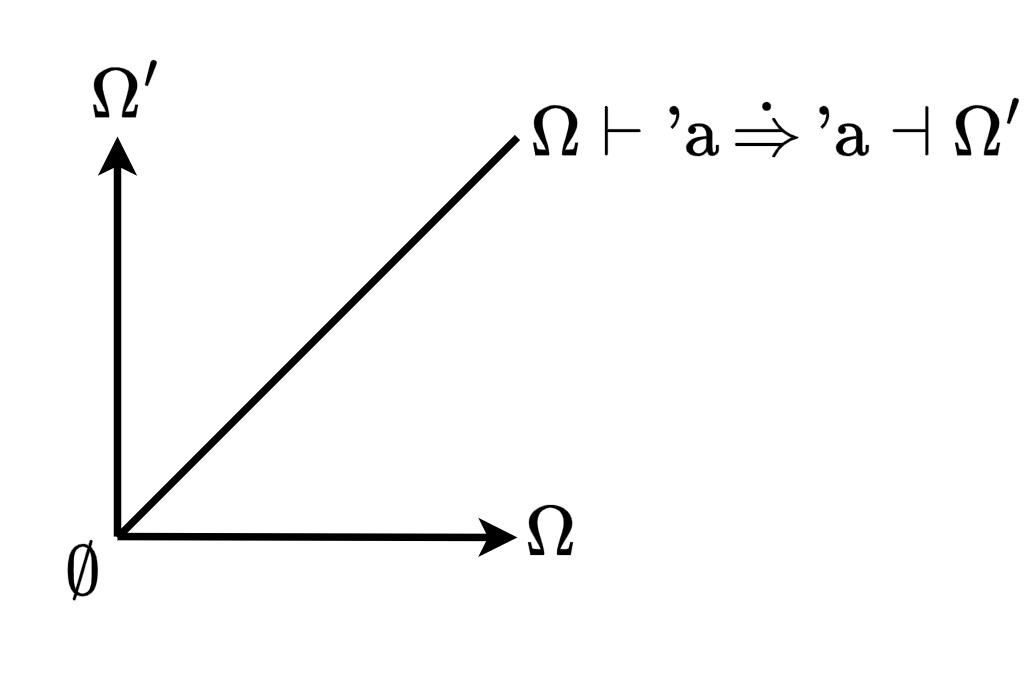
\includegraphics[width=6cm]{atomexample.png}
  Atoms leave $\Omega$ unchanged
\end{minipage}

\begin{Property}{Statement Interpretation Monotonicity}{}
  \begin{minipage}{0.6\textwidth}
    \centering
    for all $\diamond$ in $\{ \erasedreadarrow, \movearrow \}$.
    \[\inferrule{
      \Omega_0 \vdash S \subtype S' \diamond t_0 \\\\
      \Omega_1 \subtype \Omega_0
    }{}\]
    implies there exists $t_1$ s.t.
    \[\inferrule{
      \Omega_1 \vdash S \subtype S' \diamond t_1 \\\\
      \Omega_1 \vdash t_1 \subtype t_0
    }{}\]
  \end{minipage}
  \begin{minipage}{0.3\textwidth}
    \centering
    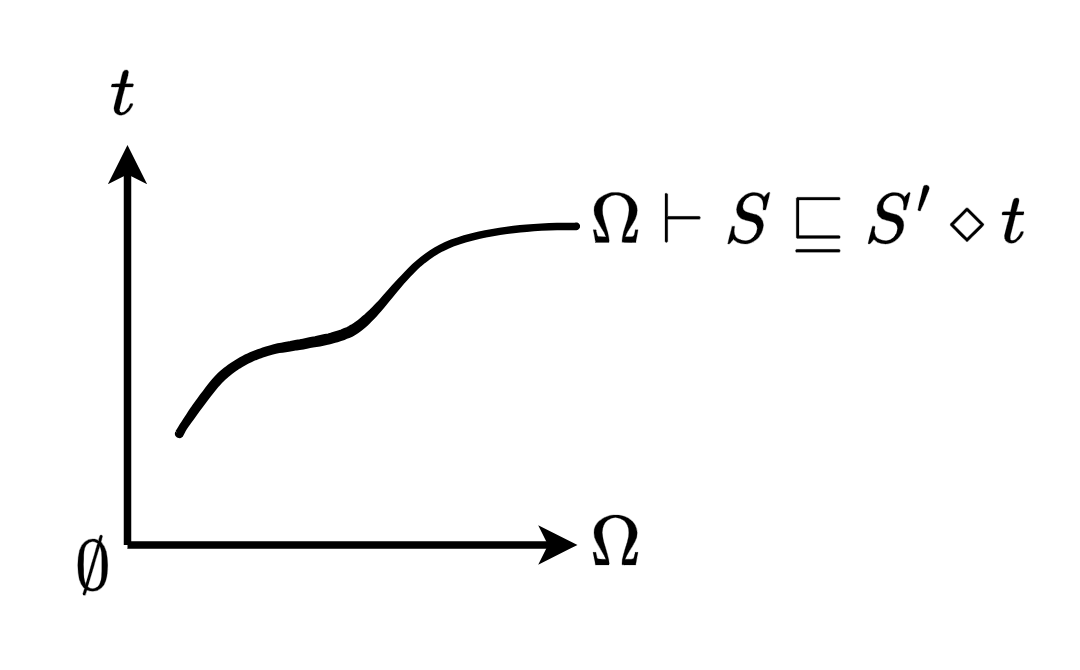
\includegraphics[width=6cm]{statementmonotonicity.png}
    Always up and right
  \end{minipage}
\end{Property}
\label{property:statementmonotonicity}

\ref{property:statementmonotonicity} states that if you narrow the environment a statement is interpreted under, it narrows the type it is interpreted to.

\begin{Property}{Expression Read Monotonicity}{}
  \begin{minipage}{0.6\textwidth}
    \centering
    for all $\diamond$ in $\{ \readarrows \}$.
    \[\inferrule{
      \Omega_0' \subtype \Omega_0 \\\\
      \Omega_0 \vdash M \diamond t \dashv \Omega_1
    }{}\]
    implies there exists a $\Omega_1'$ and $t'$ s.t.
    \[\inferrule{
      \Omega_1' \subtype \Omega_1 \\\\
      \Omega_1' \vdash t' \subtype t \\\\
      \Omega_0' \vdash M \diamond t' \dashv \Omega_1' 
    }{}\]
  \end{minipage}
  \begin{minipage}{0.3\textwidth}
    \centering
    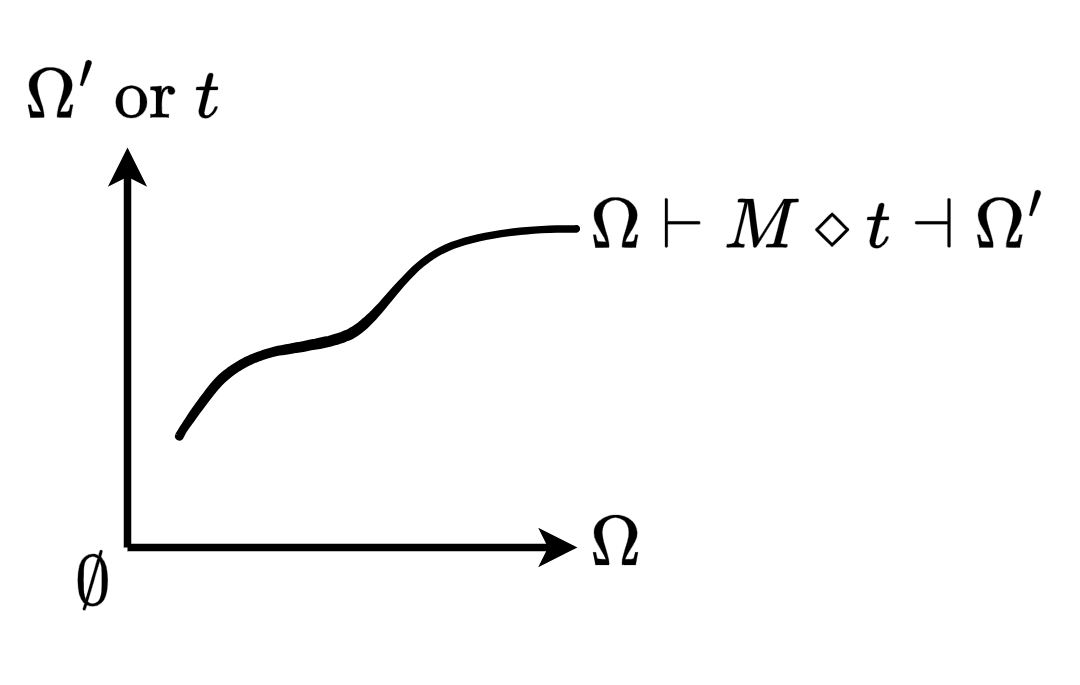
\includegraphics[width=6cm]{expressionreadmonotonicity.png}
    Always up and right
  \end{minipage}
  \label{property:expressionreadmonotonicity}
\end{Property}

\begin{Property}{Expression Write Monotonicity}{} % yes
  \begin{minipage}{0.6\textwidth}
    \centering
    for all $\diamond$ in $\{ \writearrows \}$.
    \[\inferrule{
      \Omega_0' \subtype \Omega_0 \\\\
      \Omega_0' \vdash t' \subtype t \\\\
      \Omega_0 \vdash M \diamond t \dashv \Omega_1
    }{}\]
    there exists $\Omega_1'$ s.t.
    \[\inferrule{
      \Omega_1' \subtype \Omega_1 \\\\
      \Omega_0' \vdash M \diamond t' \dashv \Omega_1' 
    }{}\]
  \end{minipage}
  \begin{minipage}{0.3\textwidth}
    \centering
    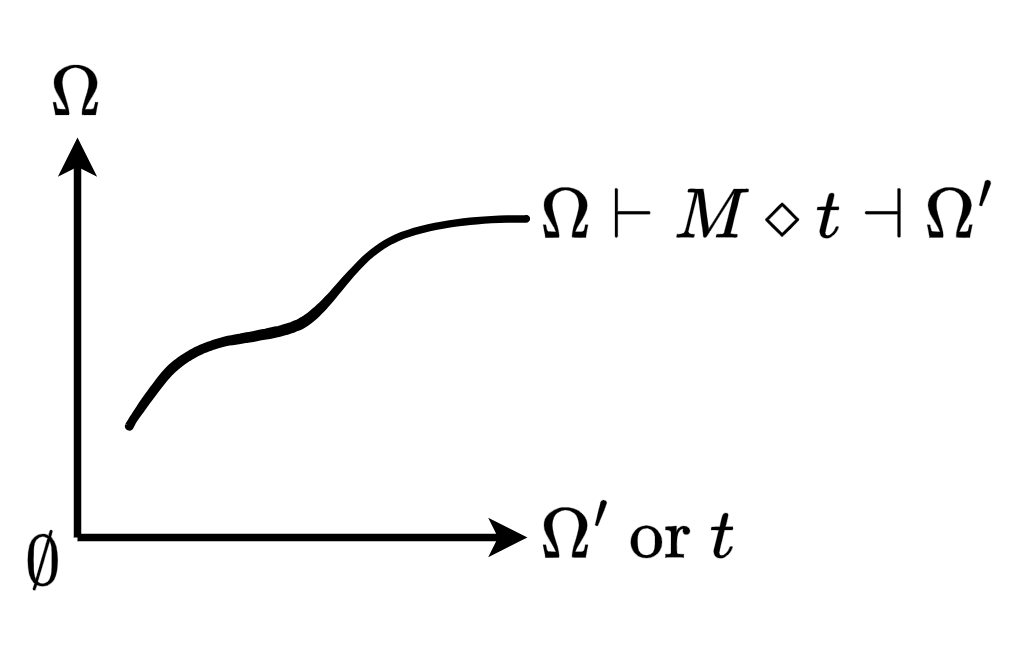
\includegraphics[width=6cm]{expressionwritemonotonicity.png}
    Always up and right
  \end{minipage}
  \label{property:expressionwritemonotonicity}
\end{Property}

\begin{Property}{Statement Bounds Respected}{} % yes
  % \begin{minipage}{0.6\textwidth}
    \centering
    for all $\diamond$ in \{ \readarrowabs, \movearrowabs \}.
    \[\inferrule{
      \Omega \vdash S \subtype S' \diamond t
    }{}\]
    there exists a $u$ s.t.
    \[\inferrule{
      \Omega \vdash S \subtype \_ \diamond u \\\\
      \Omega \vdash S' \subtype \_ \erasedreadarrow t \\\\
      \Omega \vdash u \subtype t
    }{}\]
  % \end{minipage}
  % \begin{minipage}{0.35\textwidth}
  %   \centering
  %   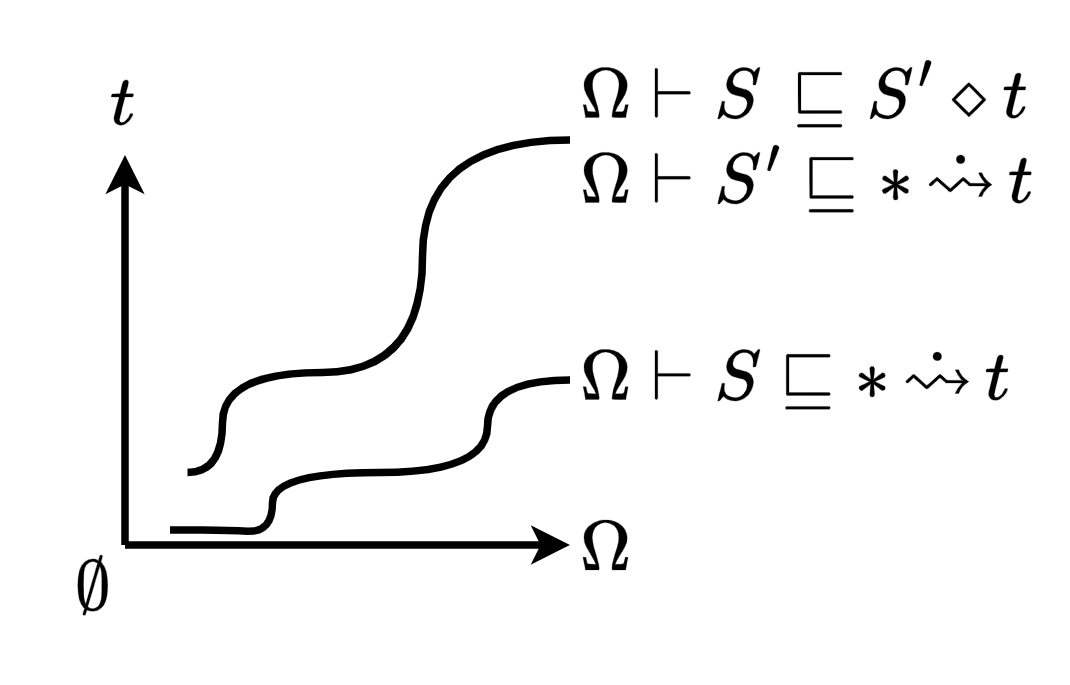
\includegraphics[width=6.5cm]{statementbounds.png}
  %   Lines never cross
  % \end{minipage}
\end{Property}
\label{theorem:statementbounds}

\subsection{Subtyping Preservation}
We introduce subtyping between terms, like so;

\noindent
\begin{Definition}[width=0.45\textwidth, nobeforeafter]{Expression Subtyping}{}
    \[\inferrule{
      \Omega \vdash M \diamond m \dashv \Omega_m \\\\
      \Omega \vdash N \diamond n \dashv \Omega_n \\\\
      \Omega_m \subtype \Omega_n \\\\
      \Omega_m \vdash m \subtype n
    }{
      \Omega \vdash M \subtype_{\diamond} N
    }\]
\end{Definition}
\hfill
\begin{Definition}[width=0.45\textwidth, nobeforeafter]{Statement Subtyping}{}
    \[\inferrule{
      \Omega \vdash S \subtype S_t \movearrowabs t
    }{
      \Omega \vdash S \subtype S_t
    }\]
\end{Definition}

\begin{Property}{Expression Subtyping Preservation}{} % yes
  \begin{minipage}{0.6\textwidth}
    \centering
    for all $\diamond$ in $\{ \movearrowabs, \readarrowabs, \erasedreadarrow \}$
    \[\inferrule{
      \Omega_0 \vdash M \subtype_{\diamond} N \\\\
      \Omega_1 \subtype \Omega_0
    }{}\]
    implies
    \[\Omega_1 \vdash M \subtype_{\diamond} N\]
  \end{minipage}
  \begin{minipage}{0.3\textwidth}
    \centering
    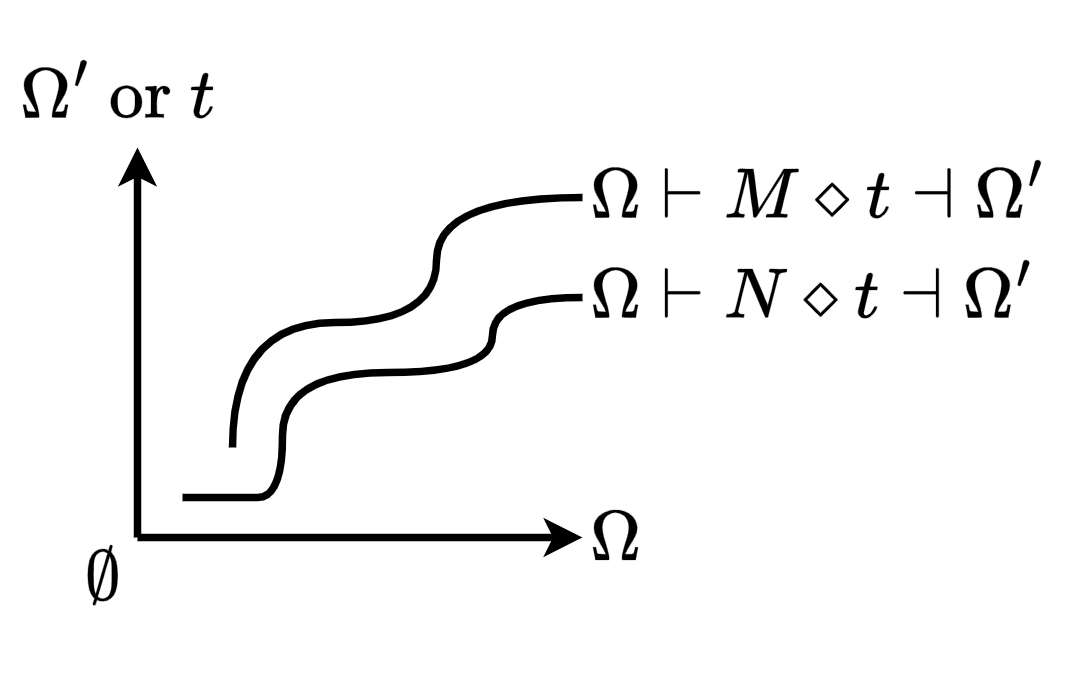
\includegraphics[width=6cm]{expressionsubtyping.png}
    Lines never cross
  \end{minipage}
\end{Property}
\label{property:expressionsubtyping}

Boolean \mono{not} counter example

The fact this does not hold is the motivation behind bounded statement interpretation because, with bounded statement interpretation, we can define statement subtyping and an equivalent subtyping preservation theorem. This is the primary reason why statements and expressions are separated from expressions.

\begin{Property}{Statement Subtyping Preservation}{} % yes
  \begin{minipage}{0.6\textwidth}
    \centering
    for all $\diamond$ in $\{ \movearrowabs, \erasedreadarrow \}$.
    \[\inferrule{
      \Omega_0 \vdash S \subtype_{\diamond} S_t \\\\
      \Omega_1 \subtype \Omega_0
    }{}\]
    implies
    \[\Omega_1 \vdash S \subtype_{\diamond} S_t \]
  \end{minipage}
  \begin{minipage}{0.3\textwidth}
    \centering
    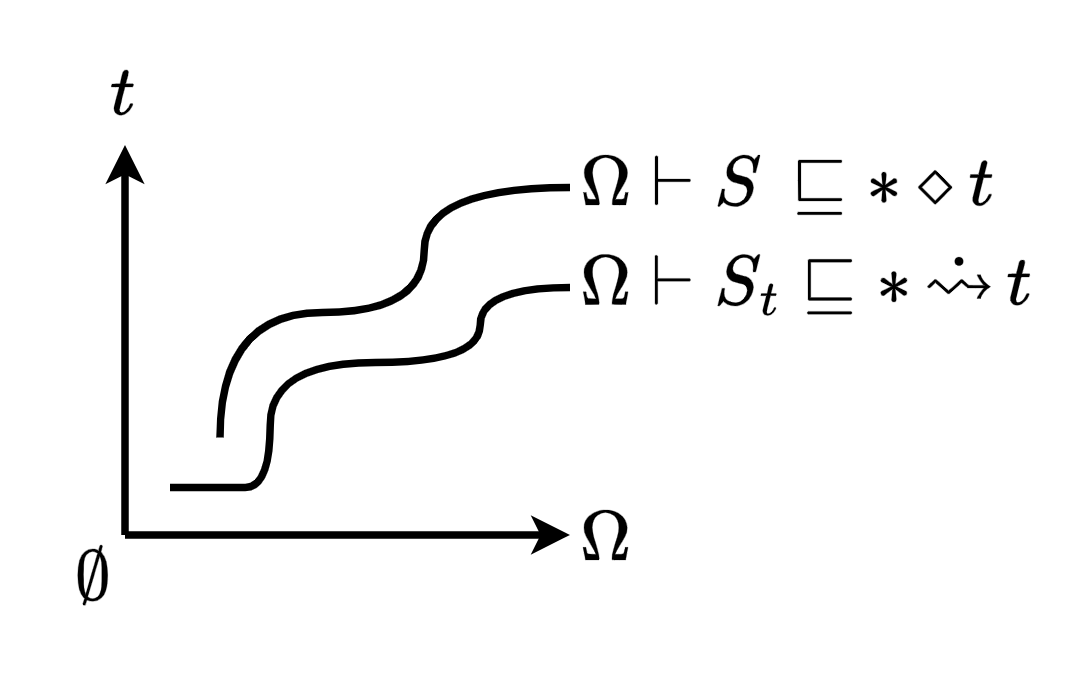
\includegraphics[width=6cm]{statementsubtyping.png}
    Lines never cross
  \end{minipage}
\end{Property}
\label{property:statementsubtyping}

\subsubsection{Statement Bound Motivation}

\begin{Definition}{Expression-Like Statement Subtyping}{}
  \[\inferrule{
    \Omega \vdash S_a \subtype \mono{*} \movearrowabs t_a \\\\
    \Omega \vdash S_b \subtype \mono{*} \movearrowabs t_b \\\\
    \Omega \vdash t_a \subtype t_b
  }{
    \Omega \vdash S_a \hat{\subtype} S_b
  }\]
\end{Definition}

\begin{Property}{Expression-Like Statement Subtyping \textbf{Non-}Preservation}{} \[
  \inferrule{
    \Omega \vdash S_a \hat{\subtype} S_b \\\\
    \Omega' \subtype \Omega
  }{}
    \text{   does not imply   }
    \Omega' \vdash S_a \hat{\subtype} S_b
  \] 
\end{Property}
\label{theorem:statementsubtypingpreservation}

\subsection{Determinism}
\todo[inline]{include or remove this section}

\subsection{Information Gain/Loss}
\begin{Property}{Read-Interpretation Widens}{} % yes
  \begin{minipage}{0.6\textwidth}
    \centering
    for all $\diamond$ in $\{ \movearrowabs, \readarrowabs, \erasedreadarrow \}$
    \[
      \inferrule{
        \Omega \vdash M \diamond t \dashv \Omega'
      }{}
      \text{   implies   }
      \Omega \subtype \Omega'
    \]
  \end{minipage}
  \begin{minipage}{0.3\textwidth}
    \centering
    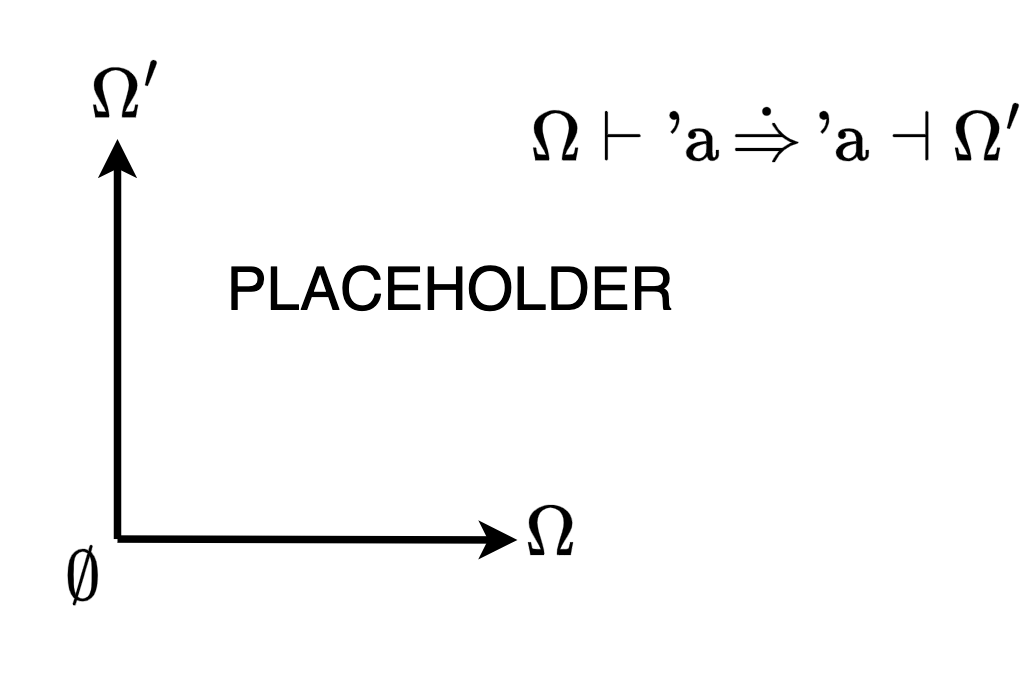
\includegraphics[width=6cm]{placeholder.png}
    Always up and right
  \end{minipage}
\end{Property}
\label{theorem:expressionreadwidens}


\begin{Property}{Write-Interpretation Narrows}{} % yes
  \begin{minipage}{0.6\textwidth}
    \centering
    for all $\diamond$ in $\{ \writearrowabs, \narrowarrowabs, \erasedwritearrow \}$
    \[
      \inferrule{
        \Omega \vdash M \diamond t \dashv \Omega'
      }{}
      \text{   implies   }
      \Omega' \subtype \Omega
    \]
  \end{minipage}
  \begin{minipage}{0.3\textwidth}
    \centering
    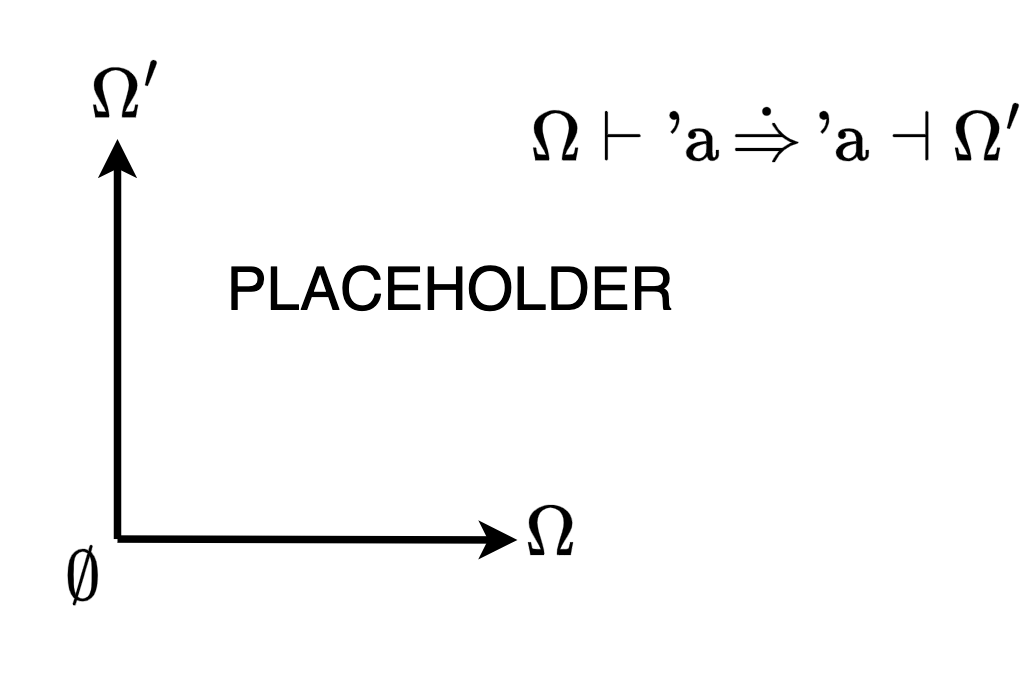
\includegraphics[width=6cm]{placeholder.png}
    Always up and right
  \end{minipage}
\end{Property}
\label{theorem:expressionwritewidens}

The narrower an environment is, the more information it contains. These two theorems state that reading from the environment always \textit{uses} information and writing to the environment \textit{adds} information.

\begin{Property}{Type Union is Precise}{}
  \[
    \Omega \vdash t_0 \sqcup t_1 = t
    \text{   iff   }
    \Omega \vdash t \subtype t_0
    \text{   or   } 
    \Omega \vdash t \subtype t_1
  \]
\end{Property}
\label{theorem:precisetypeunion}

\begin{Property}{Environment Union is \textbf{not} Precise}{}
  \ocomment{todo}
\end{Property}
\label{theorem:inpreciseenvunion}

% \begin{tcolorbox}[colback=red!5!white,colframe=red!75!black,title=Hole]
%   test
% \end{tcolorbox}

%%%%%%%%%%%%%%%%%%%%%%%%%%%%%%%%%%%%
\chapter{Evaluation}
Ochre has two goals: to allow the programmer to encode strong properties in the type system, and to be efficiently executable on hardware. Section \ref{section:performance} evaluates Ochre against the former goal, and Section \ref{section:typesystem} evaluates against the latter.

A secondary goal of this research is to make a pleasant and powerful language with useful abstractions. This is discussed in Section \ref{section:ergonomics}.

The contribution of this research is the design and specification of a language, as opposed to an implementation, so the contributions will be evaluated against how well the design \& type checking algorithm lays the foundations for a future implementation.

\section{Type System}
\label{section:typesystem}
The type system presented must reject well-formed programs, and reject ill-formed ones. This section evaluates whether or not this is the case in two distinct ways: firstly Section \ref{section:examplechecks} shows the typing rules in action for a collection of programs which should or shouldn't be accepted. Then, Section \ref{section:properties} states a set of theorems which should hold.

\section{Performance}
\label{section:performance}
\todo[inline]{maybe explicitly talk about cache coherency and pointer indirection and function pointers}
For the presented design to be good, it must describe a language with semantics that can easily be translated into efficient machine code by a compiler. This section discusses the various language features of Ochre and their performance implications.

Due to having a borrow checker, the abstract interpretation introduced in Section \ref{chapter:definition} statically determines when objects are dropped, which means it can insert any necessary memory frees into the resultant binary, removing the requirement for a garbage collector.

Being able to mutate data structures in place also allows programmers to express efficient algorithms provided they don't break the \textit{aliasing xor mutability} invariant, like Rust.

Ochre does not have native machine integers, which restricts the programmer to using Peano arithmetic or similar. This is disastrous for performance, and would not be tolerated in even the slowest languages. However, the design presented, and its type checker are perfectly compatible with integers (they would be similar to atoms), so while this work does not directly include efficient integers, I consider them compatible with it, and adding them would be a matter of engineering. The decision not to include them is discussed further in Section \ref{section:designdecisions}.

As presented, the type system does not support unboxed pairs, which means Ochre programs as currently stated have a lot of unnecessary indirection in their data structures. Much like not supporting machine integers, this is intolerable for a production systems language. However, the type system as presented is compatible with adding them in the future, and adding them at this point would detract from the core concepts. To demonstrate this compatibility, Appendix \ref{appendix:unbox} lays out a potential method for adding unboxed types.

Ochre does not have efficient contiguous arrays, which hurts the implementation of several dynamic structures, but after unboxed pairs are implemented, contiguous arrays are just many nested pairs. It is unclear how you would efficiently lookup the $n^{\text{th}}$ element in such a structure, but I am hopeful it would just be a matter of engineering/adding the right optimizations.

\chapter{Conclusion}
\section{Future Work}
\subsection{Reduce Feature Set, Increase Rigor}
Section {section:properties} attempts to argue that the system presented is sound, somewhat unconvincingly. Although I believe it could be proven by a better semanticist than myself, and/or with much more time, I think the best way of getting to that point is by reducing the feature set and progressively building them back. I suggest two such feature sets:

\subsubsection{Och}
Och would lack dependent types and mutability, but keep the core principle that terms are their own type, and subtyping/structural typing in general.

Och would have the following syntax and environment:

\begin{figure}[H]
  \arraycolsep=1pt %
  \begin{adjustwidth}{-1cm}{-1cm}
  \begin{mathpar}
  \begin{array}[t]{llll}
    M, N & ::= & & \ocomment{term} \\
    && x \mid{} y \mid{} z  & \ocomment{runtime variable} \\
    && X \mid{} Y \mid{} Z  & \ocomment{comptime variable} \\
    && \atom{a} & \ocomment{atom construction} \\
    && M\mono{,} N & \ocomment{pair construction} \\
    && \pleft{M} & \ocomment{pair left access} \\
    && \pright{M} & \ocomment{pair right access} \\
    && M N & \ocomment{application} \\
    && \mono{$M$ -> $N$} & \ocomment{abstraction} \\
    && \mono{\_} & \ocomment{uninitialised} \\
    && T\,\mono{|}\,U & \ocomment{type union} \\
    && M\mono{:}\,T & \ocomment{type constraint} \\
    && M = N & \ocomment{assignment} \\
    && \mono{match}\,M\,\{\,\overrightarrow{M'\mono{ => }S}\,\} & \ocomment{match statement} \\
  \end{array} %
  
  \begin{array}[t]{llll}
    \Omega & ::= & & \ocomment{environment} \\
    && \emptyset & \ocomment{empty env.} \\
    && \Omega, x \mapsto v & \ocomment{runtime variable} \\
    && \Omega, X \mapsto v & \ocomment{comptime variable} \\
    \\
    t, u & ::= & & \ocomment{type/value} \\
    && \{\overrightarrow{\atom{a}}\} & \ocomment{atom} \\
    && (t, u) & \ocomment{pair} \\
    && (t \rightarrow u) & \ocomment{function} \\
    && \top & \ocomment{top} \\
  \end{array}
  \end{mathpar}  
  \end{adjustwidth}
\caption{Och syntax} %
\label{fig:ochsyntax} %
\end{figure} %

Because Och does not have references or mutation, it would not need move semantics, and therefore would not need the destructive/non-destructive modality. With this change, the difference between the runtime and comptime modalities might become negligible to the point of redundancy, which would reduce the interpretation down to only the read/write and abstract/concrete modalities.

I speculate that these simplifications would make a soundness proof feasible, and undertaking such a proof effort would cause changes that would leave the language on firmer foundations.

\subsubsection{Ochr}
Once the core subtyping system is shown to be sound, useful, and implementable, dependent types should be added.

Efforts should be made to not introduce syntax into the abstract environment for the sake of calculating return types as the current version of Ochre has, as this introduces a large amount of complexity into the soundness proof and makes the re-usability of subtyping derivations very labor intensive. This could be done by having the syntax wrapped in a construct that captures the environment needed to evaluate it, similar to how Haskell functions are embedded within the definition of \mono{Value} in \cite{lohTutorialImplementationDependently2010}, Section 2.4.

Ochr would be Och extended as minimally as possible to include dependent types.

Unlike Ochre as presented, Ochr would allow for dependencies between variables in the abstract environment, which would make environment union precise. This would solve the issue of computing the join, or the "merge problem" in Mezzo \citep{protzenkoMezzoTypedLanguage2014}, and enable match statements to occur in non-terminal positions without duplication of the code afterward.

\subsection{Increase Feature Set, Increase Usability}
There are many important features missing from Ochre which will be needed in order for it to become a useful tool for formal verification. These include:

\subsubsection{Returning References From Functions}
Aeneas' method of borrow checking is compatible with returning references from functions, so that method should be portable to Ochre.

This is an extremely important feature for user-defined containers. Without references, any getter you define must move the objects out of the container, which prevents efficient in-place mutation.

\subsubsection{Performance Critical Features}
As discussed in Section \ref{section:performance}, there are a couple of features which would drastically increase the performance with relatively little effort: primitive numeric data types, and unboxed pairs.

These would be mostly a matter of engineering, and I believe would complicate the system, so just like I believe Och and Ochr should be explored fully before Ochre, I believe Ochre should be explored fully before adding these features.

\subsubsection{Ergonomic Improvements}
Functions should be able to capture non-comptime environments, as you can with closures in Rust.

Scoping does not currently respect brackets. There is no syntactic difference to the user between defining a new variable and mutating an existing one. These are not interesting for research purposes but are important for having predictable and compositional semantics.

\subsubsection{Stretch Features}
\textbf{A \mono{?} operator which passed the continuation to an expression} -  This would allow the programmer to write expressions like \mono{foo(x -> bar(y -> x + y))} as \mono{foo? + bar?}. If \mono{foo} has the type $(A \rightarrow B) \rightarrow B$, then \mono{foo?} has the type $A$.

This would be useful for defining constructs like early returns, async/await, yield/generators, and give a powerful abstraction for programmers to use in libraries, like incremental computation.

It could also have utility while using Ochre as a theorem prover because it has a very similar type signature to RAA.

\textbf{Reverse Functions} - Writing to a function application is undefined, but maybe it should be. The interpretation of writing to a function application could be to run some sort of reverse function, which determines for a given value how to write it to the argument. This could be used to define custom pattern matching.

\subsection{Undo Regrettable Design Decisions}
There are a couple of design mistakes that I would not have made with the knowledge I have now.

\textbf{Inprecise Environment Union} - Environment type union cannot be precise because dependencies between variables are not supported (see Property \ref{theorem:inpreciseenvunion} and surrounding discussion). Initially, dependencies between variables were avoided to simplify, but it turns out that not having a precise environment union introduces the requirement for statements, which complicates things much further. I hope in the future I can change this and simplify the presented system.

\textbf{Storing Terms in Abstract Environment} - The terms used to define a function or a pair are stored in the environment, so they can be re-used to extract their precise types later. They do not store the environment in which they were first evaluated. A large reason for this design decision was to support recursion efficiently; take the following definition of Peano naturals:

\begin{minted}[mathescape]{rust}
  Nat = ('zero, 'unit) | ('succ, Nat);
  Nat.1.1.1.1.0; // $\text{perfectly valid, and equal to } \{ \atom{zero}, \atom{succ} \} $
\end{minted}

When the right-hand side of the assignment is evaluated, \mono{Nat} is mapped to $\top$ in the environment, to reflect the fact we do not yet know anything about \mono{Nat}. Right-element access then re-executes the \mono{Nat} term, with a narrower context that has a more precise definition of \mono{Nat}.

This takes advantage of the fact that it is evaluated with a more accurate environment later, so I could not remove this immediately, but I believe with future work it could be removed.

\subsection{Implementation}
The goal of this project is to enable formal verification of low-level systems code. In order to do that Ochre must have an implementation, and be usable.

To do this I would implement Ochre in a Rust macro, so it could be invoked as such:

\begin{minted}{rust}
fn main() {
  let result = ochre! {
    Nat = ('zero, 'unit) | ('succ, Nat);
    add(x: &Nat, y: &Nat): Nat = {
      match x {
        ('zero, 'unit) => ('zero, 'unit),
        ('succ, px) => ('succ, add(px, y))
      }
    };
    one = ('succ, ('zero, 'unit));
    two = ('succ, ('succ, ('zero, 'unit)));
    add(&one, &two)
  };

  println!("{}", result); // ('succ, ('succ, ('succ, ('zero, 'unit))))
}
\end{minted}

And potentially allow importing of pure Ochre files from this macro, like such:

\begin{minted}{rust}
  fn main() {
    let result = ochre! { import("./add.oc") };
  
    println!("{}", result); // ('succ, ('succ, ('succ, ('zero, 'unit))))
  }
\end{minted}

The Rust library which defines this macro could also define traits (type classes) that allow the programmer to define how Rust types are converted to and from Ochre types so that they can pass them to Ochre functions, and use the results in Rust.

The parser for a large subset of a previous version of Ochre is implemented in this way, and code generation/abstract interpretation for a few simple constructs (assignment, atoms, pairs) is implemented, but for this project I decided to prioritize the theory work.

With this interface, programmers could take an existing Rust codebase, and incrementally convert it to Ochre as and when they need stronger properties about their program proven.

% \section{Ergonomics}
% \todo[inline]{implement}
% \todo[inline]{compare with ATS, Low*, and Aeneas, although this might be very tricky beyond toy examples}

%%%%%%%%%%%%%%%%%%%%%%%%%%%%%%%%%%%%
% \chapter{Ethical Issues}
% % Ethics checklist: https://wiki.imperial.ac.uk/display/docteaching/Ethics+Process
% I do not foresee any ethical issues arising from this project.

%%%%%%%%%%%%%%%%%%%%%%%%%%%%%%%%%%%%
%% Bibliography
\bibliographystyle{plainnat}
\bibliography{references}

\appendix 
\addcontentsline{toc}{chapter}{APPENDICES}

\chapter{Appendicies}
\section{Formal Verification using (Dependent) Types}
\label{verificationwithtypes}

The primary motivation behind adding dependent types to a language is so you can perform theorem proving/formal verification in the type system. In some languages, like Lean, this is done to mechanize mathematical proofs to prevent errors and/or shorten the review process; in other languages, like F*, Idris or ATS this is done to allow the programmer to reason about the runtime properties of their programs. However, they are all just pure functional languages with dependent types, whether you choose to use this expressive power for maths or programs the underlying type system is the same.

So the question is how can you represent logical statements as (potentially dependent) types and use the type checker to prove them? This is best understood via a simpler version: proving logical tautologies using Haskell's type system.

\subsubsection{Boolean Tautologies in Haskell}
The Curry-Howard correspondence states there is an equivalence between the theory of computation, and logic. Specifically: types are analogous to statements, and terms (values) are analogous to proofs. Under this analogy, $5 : \mathbb{N}$ states that $5$ is a proof of $\mathbb{N}$.

We can use this to represent logical statements as types. Here is how various constructs in logic translate over to types (given in Haskell).

\begin{tabularx}{\textwidth}{ X|X|X }
  Logical Statement & Equivalent Haskell Type & Explanation \\
  \hline \\
  $\top$ & \verb|()| & Proving true is trivial, so unit type. \\
  $\bot$ & \verb|!| & There exists no proof of false, so empty type. \\
  $a \Rightarrow b$ & \verb|a -> b| & If you have a proof of $a$, you can use it to construct a proof of $b$. \\
  $a \wedge b$ & \verb|(a, b)| & A proof of $a$ and a proof of $b$ combined into one proof. \\
  $a \vee b$ & \verb|Either a b| & This proof was either constructed in the presence of a proof of $a$ or a proof of $b$.
\end{tabularx}

For example, to prove the logical statement $(a \wedge b) \Rightarrow a$, we must define a Haskell term with type \verb|(a, b) -> a|, which can be done as such:

\begin{lstlisting}
proof :: (a, b) -> a
proof (a, b) = a
\end{lstlisting}

For another example, we can prove $((a \wedge b) \vee (a \wedge c)) \Rightarrow (a \wedge (b \vee c))$, which you might want to convince yourself of separately before moving on, by providing a Haskell term of type \verb|Either (a, b) (a, c) -> (a, Either b c)|.

\begin{lstlisting}
proof' :: Either (a, b) (a, c) -> (a, Either b c)
proof' (Left (a, b)) = (a, Left b)
proof' (Right (a, c)) = (a, Right c)
\end{lstlisting}

% We now set out to represent statements in logic as types, and their proofs as terms.
% \begin{itemize}
%   \item A proof of $true$ should be trivial, just by knowing that we are trying to prove $true$ should be enough for us to construct the proof. For this reason, we choose to represent $true$ as the type with a single term, $\top$; otherwise known as $1$ or $()$ (``unit''). There is exactly 1 term of type $\top$, which is also denoted as whatever the type is. E.g. in Haskell \verb|(): ()|. This means that whenever we need to generate a proof of $true$, we can do so trivially because the proof is $()$.
%   \item A proof of $false$ should be impossible since $false$ can never be proven true, fso we represent it with an empty type, $\bot$; also known as $0$ or $!$. There are no terms of type $\bot$.
%   \item Logical implication, $a \rightarrow b$ means if we're given a proof of $a$, and can derive a proof of $b$, we have proven $a \rightarrow b$. It is as though the proof is taking another proof as input. We represent logical implication as the function type, also denoted by $\rightarrow$. For instance, if we could make a type-checking term \verb|f| of type \verb|() -> ()| in Haskell, we would have proven that $true \rightarrow true$. This is trivial with \verb|f () = ()|.
%   \item Conjunction, $a \wedge b$ (logical and), means we have proven both $a$ and $b$. We represent this with the pair $(a, b)$. To get a term of type $(a, b)$ we must have both a term of type $a$ and a term of type $b$, which is analogous to having a proof of $a$ \textit{and} a proof of $b$.
%   \item Disjunction, $a \vee b$ (logical or), means we have either proven $a$ or $b$. We represent this with the slightly less mathematical \verb|Either a b|. If we have a term of type $a$, we can produce an \verb|Either a b| with \verb|Left a|, and if we have a term of type $b$ we can produce an \verb|Either a b| with \verb|Right b|. This is analogous to having either a proof of $a$, \textit{or} a proof of $b$. 
% \end{itemize}

With this we can construct proofs for logical tautologies, but how do we go further and construct proofs for statements like ``If you get any number and double it, you get an even number''.

\subsubsection{Dependent Types are Quantifiers}
Let's now define a function $even$ which returns a type, such that any term of type $even(n)$ is proof that $n$ is even. To do this, $even$ returns a \textit{type}: $\top$ if $n$ is even, $\bot$ otherwise. I.e. $even(4) = \top$ and $even(5) = \bot$. The logical statement $\forall n : \mathbb{Z}. even(2n)$ can be represented by the type $(n: \mathbb{Z}) \rightarrow even(2 * n)$. If we had a term of this type, we could give it any integer $n$, and it would return proof that $2n$ is even.

This cannot be represented in Haskell, because $(\textbf{n}: \mathbb{Z}) \rightarrow even(2 * \textbf{n})$ is a dependent type, hence we need a dependently typed language like Agda. This is an example of Haskell's non-dependent type system not being able to express quantifiers like $\forall$ or $\exists$ over values.

% this is optional section
% types are statements, programs are proofs
% normal tautologies in Haskell
% how pi and sigma types denote qualifiers

% what is formal verification
% outline of various methods for doing it

\section{Supporting Unboxed Pairs}
\label{appendix:unbox}
While atoms, functions, and references are unboxed in Ochre, pairs are always heap-allocated. As discussed in Section \ref{section:performance}, this will hinder the performance of compiled Ochre programs. This appendix lays out a rough plan for adding unboxed types to the formal semantics for Ochre, to make the point that the research as presented is compatible with such an extension.

A potential method of adding unboxed pairs:

\begin{enumerate}
  \item \textbf{Add $\kw{box} \, t$, a new type which represents an explicit heap allocation}, along with corresponding constructors and eliminators. This is required so the programmer can heap allocate objects whose size is not comptime known.
  \item \textbf{Edit the abstract interpretations to pass around (type, size) pairs instead of just types}. This would involve all read arrows returning the size of the value being read, and all write arrows taking the size of the data being written.
  
  Set the size of pairs to the sum of the size of the elements in the pair. Because the type of the right-hand side can depend on the left, this can cause some sizes to be unknown. Because of this, arrows may return an unknown size, and if the user needs to put something of unknown size on the stack, they must put it in a box.

  The size of a match statement is the largest size of any of its branches.
\end{enumerate}

% With pairs being boxed, this isn't required, because every type is one machine word long (pairs are a pointer to a heap allocation of two values, and pointers are a single word). The definition for size on statements and values would look something like the 

% \begin{figure}[H]
%   \small
%   \centering
%   \begin{mathpar}
%     \begin{array}{c|c}
%       t & \odef{\kw{size}}{t} \\
%       \hline

%       \\(t, T \rightarrow S) &
%       \inferrule{
%         \Omega \vdash \size{t} = l \\\\
%         \Omega \vdash T \erasedwritearrow t \dashv \Omega' \\\\
%         \Omega' \vdash \size{S} = r
%       }{
%         \Omega \vdash \size{(t, T \rightarrow S)} = l + r
%       } \\

%       \\M &
%       \inferrule{
%         M \textit{is not a pair}
%       }{
%         \Omega \vdash \size{M} = 1
%       } \\

%     \end{array}

%     \begin{array}{c|c}
%       S & \odef{\kw{size}}{S} \\
%       \hline

%       \\M &
%       \inferrule{
%         \\
%       }{
%         \Omega \vdash 
%       } \\

%       \\M &
%       \inferrule{
%         M \textit{is not a pair}
%       }{
%         \size{M} = 1
%       } \\

%     \end{array}
%   \end{mathpar}
% \end{figure}

\section{Derivations}
\subsection{Hello World Program Derivation}
\label{appendix:helloworldderivation}
This appendix gives a derivation for the Hello World Program shown in Listing \ref{listing:helloworld}.

Derivation:

{\smaller
\[\begin{array}{ll}
  \Omega_0 \vdash L_2\mono{;}L_3\mono{;}L_4\mono{;}L_5\mono{;}L_7 \subtype \mono{*} \movearrowabs (\atom{hello}, \mono{\_} \rightarrow \atom{world}) &
  \Omega_0 = \emptyset \\

  % pair = ('world, 'hello)
  \otab \ocomment{\mono{pair = ('world, 'hello)}} \\
  \otab \Omega_0 \vdash \mono{('world, 'hello)} \movearrowabs (\atom{world}, \mono{\_} \rightarrow \atom{hello}) \\
  \otab \otab \Omega_0 \vdash \mono{'world} \movearrowabs \atom{world} \\
  \otab \otab \Omega_0 \vdash \mono{'hello} \movearrowabs \atom{hello} \\
  \otab\Omega_0 \vdash \mono{pair} \writearrowabs (\atom{world}, \mono{\_} \rightarrow \atom{hello}) \dashv \Omega_1 &
   \langle\text{Rearrange-Before}\rangle \\
  \otab\otab \Omega_0 \rearrangearrow \Omega_0' &
   \langle\text{Allocate}\rangle \\
  \otab\otab\otab \Omega_0' = \Omega_0,\absmapm{pair}{\top} &
   \Omega_0' = \emptyset, \absmapm{pair}{\top} \\
  \otab \otab \Omega_0' \vdash \mono{pair} \writearrowabs (\atom{world}, \mono{\_} \rightarrow \atom{hello}) \dashv \Omega_1 \\
  \otab\otab\otab \Omega_1 = \Omega_0'\left[\dfrac{\absmapm{pair}{(\atom{world}, \mono{\_} \rightarrow \atom{hello})}}{\absmapm{pair}{\top}}\right] &
   \Omega_1 = \emptyset,\absmapm{pair}{(\atom{world}, \mono{\_} \rightarrow \atom{hello})}\\
  \otab \Omega_1 \vdash L_3\mono{;}L_4\mono{;}L_5\mono{;}L_7 \subtype \mono{*} \movearrowabs (\atom{hello}, \mono{\_} \rightarrow \atom{world}) \\
  \otab \otab \mathcal{D}_3 \\

\end{array}\]
\[\begin{array}{ll}
  \mathcal{D}_3 = \\\\

  \Omega_1 \vdash L_3\mono{;}L_4\mono{;}L_5\mono{;}L_7 \subtype \mono{*} \movearrowabs (\atom{hello}, \mono{\_} \rightarrow \atom{world}) \\
  % temp = pair.0
  \otab \ocomment{\mono{temp = pair.0}} \\
  % read right
  \otab \Omega_1 \vdash \mono{pair.0} \movearrowabs \atom{world} \dashv \Omega_1'' \\
  \otab \otab \Omega_1 \vdash \mono{pair} \movearrowabs (\atom{world}, \mono{\_} \rightarrow \atom{hello}) \dashv \Omega_1' \\
  \otab\otab\otab \Omega_1' = \Omega_1\left[\dfrac{\absmapm{pair}{\top}}{\absmapm{pair}{(\atom{world}, \mono{\_} \rightarrow \atom{hello})}}\right] &
    \Omega_1' = \emptyset, \absmapm{pair}{\top} \\
  \otab \otab \Omega_1' \vdash \oleft{(\atom{world}, \mono{\_} \rightarrow \atom{hello})} = \atom{world} \\
  \otab \otab \Omega_1' \vdash \oright{(\atom{world}, \mono{\_} \rightarrow \atom{hello})} = \atom{hello} \\
  \otab \otab \Omega_1' \vdash \mono{pair} \writearrowabs (\top, \mono{\_} \rightarrow \atom{hello}) \dashv \Omega_1'' \\
  \otab\otab\otab \Omega_1'' = \Omega_1'\left[\dfrac{\absmapm{pair}{(\top, \mono{\_} \rightarrow \atom{hello})}}{\absmapm{pair}{\top}}\right] &
    \Omega_1'' = \emptyset,\absmapm{pair}{(\top, \mono{\_} \rightarrow \atom{hello})} \\
  % write to left
  \otab\Omega_1'' \vdash \mono{temp} \writearrowabs \atom{world} \dashv \Omega_2 &
    \langle\text{Rearrange-Before}\rangle \\
  \otab\otab \Omega_1'' \rearrangearrow \Omega_1''' &
    \langle\text{Allocate}\rangle \\
  \otab\otab\otab \Omega_1''' = \Omega_1'', \absmapm{temp}{\top} &
    \Omega''' = \emptyset,\absmapm{pair}{(\top, \mono{\_} \rightarrow \atom{hello})}, \absmapm{temp}{\top} \\
  \otab\otab \Omega_2 = \Omega_1'''\left[\dfrac{\absmapm{temp}{\atom{world}}}{\absmapm{temp}{\top}}\right] &
    \Omega_2 = \emptyset,\absmapm{pair}{(\top, \mono{\_} \rightarrow \atom{hello})}, \absmapm{temp}{\atom{world}} \\
  \otab \Omega_2 \vdash L_4\mono{;}L_5\mono{;}L_7 \subtype \mono{*} \movearrowabs (\atom{hello}, \mono{\_} \rightarrow \atom{world}) \\
  \otab\otab \mathcal{D}_4 \\

\end{array}\]
\[\begin{array}{ll}
  \mathcal{D}_4 = \\\\

  \Omega_2 \vdash L_4\mono{;}L_5\mono{;}L_7 \subtype \mono{*} \movearrowabs (\atom{hello}, \mono{\_} \rightarrow \atom{world}) \\
  % pair.0 = pair.1
  \otab \ocomment{\mono{pair.0 = pair.1}} \\
  % read right
  \otab \Omega_2 \dashv \mono{pair.1} \movearrowabs \atom{hello} \dashv \Omega_2' \\
  \otab\otab \ocomment{Similar to $\Omega_1 \vdash \mono{pair.0} \movearrowabs \atom{world} \dashv \Omega_1''$} &
    \Omega_2' = \emptyset, \absmapm{pair}{(\top, \mono{\_} \rightarrow \top)}, \absmapm{temp}{\atom{world}} \\
  \otab \Omega_2' \dashv \mono{pair.0} \writearrowabs \atom{hello} \dashv \Omega_3 \\
  \otab \otab \Omega_2' \vdash \mono{pair} \movearrowabs (\top, \mono{\_} \rightarrow \top) \dashv \Omega_2'' \\
  \otab\otab\otab \Omega_2'' = \Omega_2'\left[\dfrac{\absmapm{pair}{\top}}{\absmapm{pair}{(\top, \mono{\_} \rightarrow \top)}}\right] &
    \Omega_2'' = \emptyset, \absmapm{pair}{\top}, \absmapm{temp}{\atom{world}} \\
  \otab \otab \Omega_2'' \vdash \oleft{(\top, \mono{\_} \rightarrow \top)} = \top \\
  \otab \otab \Omega_2'' \vdash \oright{(\top, \mono{\_} \rightarrow \top)} = \top \\
  \otab \otab \Omega_2'' \vdash \mono{pair} \writearrowabs (\atom{hello}, \mono{\_} \rightarrow \top) \dashv \Omega_2''' \\
  \otab\otab\otab \Omega_3 = \Omega_2''\left[\dfrac{\absmapm{pair}{(\atom{hello}, \mono{\_} \rightarrow \top)}}{\absmapm{pair}{\top}}\right] &
    \Omega_3 = \emptyset,\absmapm{pair}{(\atom{hello}, \mono{\_} \rightarrow \top)}, \absmapm{temp}{\atom{world}} \\
  \otab \Omega_3 \vdash L_5\mono{;}L_7 \subtype \mono{*} \movearrowabs (\atom{hello}, \mono{\_} \rightarrow \atom{hello}) \\
  \otab\otab \mathcal{D}_5 \\
\end{array}\]

\[\begin{array}{ll}
  \mathcal{D}_5 = \\\\

  \Omega_3 \vdash L_5\mono{;}L_7 \subtype \mono{*} \movearrowabs (\atom{hello}, \mono{\_} \rightarrow \atom{hello}) \\
  % pair.1 = temp
  \otab \ocomment{\mono{pair.1 = temp}} \\
  \otab \Omega_3 \vdash \mono{temp} \movearrowabs \atom{world} \dashv \Omega_3' \\
  \otab \Omega_3' = \Omega_3\left[\dfrac{\absmapm{temp}{\top}}{\absmapm{temp}{\atom{world}}}\right] &
  \otab \Omega_3' = \emptyset, \absmapm{pair}{(\atom{hello}, \mono{\_} \rightarrow \top)}, \absmapm{temp}{\top} \\
  \otab \Omega_3' \vdash \mono{pair.1} \writearrowabs \atom{world} \dashv \Omega_4 \\
  \otab \ocomment{Similar to $\Omega_2' \dashv \mono{pair.0} \writearrowabs \atom{hello} \dashv \Omega_3$} &
  \otab \Omega_4 = \emptyset,\absmapm{pair}{(\atom{hello}, \mono{\_} \rightarrow \atom{world})}, \absmapm{temp}{\top} \\
  \otab \Omega_4 \vdash L_7 \subtype \mono{*} \movearrowabs (\atom{hello}, \mono{\_} \rightarrow \atom{world}) \\
  \otab\otab \mathcal{D}_7 \\
\end{array}\]

\[\begin{array}{ll}
  \mathcal{D}_7 = \\\\

  \otab \Omega_4 \vdash L_7 \subtype \mono{*} \movearrowabs (\atom{hello}, \mono{\_} \rightarrow \atom{world}) \\
  % pair
  \otab \ocomment{\mono{pair}} \\
  \otab \Omega_4 \vdash \mono{pair} \movearrowabs (\atom{hello}, \mono{\_} \rightarrow \atom{world}) \dashv \Omega_4' \\
  \otab \otab \Omega_4' = \Omega_4\left[\dfrac{\absmapm{pair}{\top}}{\absmapm{pair}{(\atom{hello}, \mono{\_} \rightarrow \atom{world})}}\right] &
    \Omega_4' = \emptyset, \absmapm{pair}{\top}, \absmapm{temp}{\top} \\
  \otab \Omega_4' \vdash \drop{} \\
  \otab \otab \emptyset, \absmapm{pair}{\top}, \absmapm{temp}{\top} \vdash \kw{drop} \\
  \otab \otab\otab \emptyset, \absmapm{pair}{\top} \vdash \drop{\top} \\
  \otab \otab\otab \emptyset, \absmapm{pair}{\top} \vdash \drop{} \\
  \otab \otab\otab\otab \emptyset \vdash \drop{\top} \\
  \otab \otab\otab\otab \emptyset \vdash \drop{} \\

\end{array}\]
}

\subsection{Mutating a Dependent Pair}
\label{appendix:mutateddependentderivation}
This appendix shows the derivation which type checks the definition of the \mono{overwrite} function from Listing \ref{listing:mutatedependent}.

{
  \smaller
  \[\begin{array}{ll}
    \multicolumn{2}{l}{ 
      $$\Omega_1 \vdash \mono{(p:\&mut Same) -> 'unit \{*p.0 = 'a; *p.1 = 'a; 'unit\}} \movearrowabs (\mono{p:\&mut Same}) \rightarrow \mono{'unit}$$
    } \\
  
    \otab\Omega_1 \vdash \mono{(p:\&mut Same)} \maxarrow{\writearrowabs} \borrowm{l}{p_0} \dashv \Omega_{10} \\
    \otab\otab \Omega_1 \vdash \mono{\&mut Same} \erasedreadarrow \borrowm{l}{p_0} \dashv \Omega_1' \\
    \otab\otab\otab \Omega_1 \vdash \mono{Same} \erasedreadarrow p_0 \\
    \otab\otab\otab\otab \absmapm{Same}{p_0} \in \Omega_1 &
      p_0 = (\{\atom{a}, \atom{b}\}, L \rightarrow L) \\
    \otab\otab\otab \Omega_1' = \Omega_1, \absmap{l}{p_0} &
      \Omega_1' = \Omega_1, \absmap{l}{p_0} \\
    \otab\otab \Omega_1' \vdash \mono{p} \writearrowabs \borrowm{l}{p_0} \dashv \Omega_{10} &
      \langle\text{Rearrange-Before}\rangle \\
    \otab\otab\otab \Omega_1' \rearrangearrow \Omega_1'' &
      \langle\text{Allocate}\rangle \\
    \otab\otab\otab\otab \Omega_1'' = \Omega_1', \absmapm{p}{\top} &
      \Omega_1'' = \Omega_1', \absmapm{p}{\top} \\
    \otab\otab\otab \Omega_1'' \vdash \mono{p} \writearrowabs \borrowm{l}{p_0} \dashv \Omega_{10} \\
    \otab\otab\otab\otab \Omega_{10} = \Omega_1'\left[\dfrac{\absmapm{p}{\borrowm{l}{p_0}}}{\absmap{p}{\top}}\right] &
      \Omega_{10} = \Omega_1', \absmapm{p}{\borrowm{l}{p_0}} \\
    
    \otab \Omega_{10} \vdash \mono{*p.0 = 'a; *p.1 = 'a; 'unit} \subtype \mono{'unit} \movearrowabs \atom{unit} \\
    \otab\otab \mathcal{D}_{10}
  \end{array}\]
  \[\begin{array}{ll}
    \mathcal{D}_{10} = \\\\

    \Omega_{10} \vdash \mono{*p.0 = 'a; *p.1 = 'a; 'unit} \subtype \mono{'unit} \movearrowabs \atom{unit}
    \otab \Omega_{10} \vdash \mono{'a} \movearrowabs \atom{a} \\
    \otab \Omega_{10} \vdash \mono{*p.0} \writearrowabs \atom{a} \dashv \Omega_{11} &
      \langle\text{Rearrange-Before}\rangle \\
    \otab \otab \Omega_{10} \rearrangearrow \Omega_{10}' \, \ocomment{must set $*p.0$ to $\top$ to write} &
      \langle\text{Type-Widen}\rangle \\
    \otab \otab\otab \Omega_{10}' = \Omega_{10}\left[\dfrac{\absmapm{p}{\borrowm{l}{p_1}}}{\absmapm{p}{\borrowm{l}{p_0}}}\right] &
      \Omega_{10}' = \Omega_1', \absmap{p}{\borrowm{l}{p_1}} \\
    \otab \otab\otab \Omega_{10} \vdash \borrowm{l}{p_0} \subtype \borrowm{l}{p_1}  &
      p_1 = (\top, \mono{\_} \rightarrow \{\atom{a}, \atom{b}\}) \\
    \otab \otab\otab\otab \Omega_{10} \vdash p_0 \subtype p_1 \\
    \otab \otab\otab\otab\otab \Omega_{10} \vdash \{\atom{a}, \atom{b}\} \subtype \top \\
    \otab \otab\otab\otab\otab \Omega_{10} \vdash \comptime{} \dashv \Gamma_1 &
      \Gamma_1 = \Omega_1,\absmapm{L}{\top} \\
    \otab \otab\otab\otab\otab \Gamma_1 \vdash \mono{\_} \erasedwritearrow \top \\
    \otab \otab\otab\otab\otab \Gamma_1 \vdash \mono{L} \erasedwritearrow \{\atom{a}, \atom{b}\} \dashv \Gamma_1' \\
    \otab \otab\otab\otab\otab\otab \Gamma_1' = \Gamma_1\left[\dfrac{\absmapm{L}{\{\atom{a}, \atom{b}\}}}{\absmapm{L}{\top}}\right] \\
    \otab \otab\otab\otab\otab \Gamma_1' \vdash \mono{L} \subtype \{\atom{a}, \atom{b}\} \erasedreadarrow \{\atom{a}, \atom{b}\} \\
    \otab \otab\otab\otab\otab\otab \Gamma_1' \vdash L \erasedreadarrow \{\atom{a}, \atom{b}\} \\
    \otab \otab\otab\otab\otab\otab\otab \absmapm{L}{\{\atom{a}, \atom{b}\}} \in \Gamma_1' \\
    \otab \otab\otab\otab\otab\otab \Gamma_1' \vdash \{\atom{a}, \atom{b}\} \erasedreadarrow \{\atom{a}, \atom{b}\} \\
    \otab \otab\otab\otab\otab\otab \Gamma_1' \vdash \{\atom{a}, \atom{b}\} \subtype \{\atom{a}, \atom{b}\} \\
    \otab \otab\otab\otab\otab\otab\otab \{\atom{a}, \atom{b}\} \subseteq \{\atom{a}, \atom{b}\} \\
    \otab \otab \Omega_{10}' \vdash \mono{*p.0} \writearrowabs \atom{a} \dashv \Omega_{11} \, \ocomment{write to \mono{*p.0}} \\
    \otab \otab\otab \Omega_{10}' \vdash \mono{*p} \movearrowabs p_1 \dashv \Omega_{10}''' \\
    \otab \otab\otab\otab \Omega_{10}' \vdash \mono{p} \movearrowabs \borrowm{l}{p_1} \vdash \Omega_{10}'' \\
    \otab \otab\otab\otab\otab \Omega_{10}'' = \Omega_{10}'\left[\dfrac{\absmapm{p}{\top}}{\absmapm{p}{p_1}}\right] &
      \Omega_{10}'' = \Omega_1',\absmapm{p}{\top} \\
    \otab \otab\otab\otab \Omega_{10}'' \vdash \mono{p} \writearrowabs \borrowm{l}{\top} \vdash \Omega_{10}''' \\
    \otab \otab\otab\otab\otab \Omega_{10}''' = \Omega_{10}''\left[\dfrac{\absmapm{p}{\borrowm{l}{\top}}}{\absmapm{p}{\top}}\right] &
      \Omega_{10}''' = \Omega_1',\absmapm{p}{\borrowm{l}{\top}} \\
    \otab \otab\otab \Omega_{10}''' \vdash \oleft{p_1} = \top \\
    \otab \otab\otab \Omega_{10}''' \vdash \oright{p_1} = \{\atom{a}, \atom{b}\} \\
    \otab \otab\otab \Omega_{10}''' \vdash \mono{*p} \writearrowabs p_2 \dashv \Omega_{11} &
      p_2 = (\atom{a}, \mono{\_} \rightarrow \{\atom{a}, \atom{b}\}) \\
    \otab \otab\otab\otab \Omega_{10}''' \vdash \mono{p} \movearrowabs \borrowm{l}{\top} \dashv \Omega_{10}'''' \\
    \otab \otab\otab\otab\otab \Omega_{10}'''' = \Omega_{10}'''\left[\dfrac{\absmapm{p}{\top}}{\absmap{p}{\borrowm{l}{\top}}}\right] &
      \Omega_{10}'''' = \Omega_1',\absmapm{p}{\top} \\
    \otab \otab\otab\otab \Omega_{10}'''' \vdash \mono{p} \writearrowabs \borrowm{l}{p_2} \dashv \Omega_{11} \\
    \otab \otab\otab\otab\otab \Omega_{11} = \Omega_{10}''''\left[\dfrac{\absmapm{p}{\borrowm{l}{p_2}}}{\absmap{p}{\top}}\right] &
      \Omega_{11} = \Omega_1', \absmapm{p}{\borrowm{l}{p_2}} \\
  
    \otab \Omega_{11} \vdash \mono{*p.1 = 'a; 'unit} \subtype \mono{'unit} \movearrowabs \atom{unit} \\
    \otab\otab \mathcal{D}_{11} \\
  \end{array}\]
    
  \[\begin{array}{ll}
    \mathcal{D}_{11} = \\\\

    \Omega_{11} \vdash \mono{*p.1 = 'a; 'unit} \subtype \mono{'unit} \movearrowabs \atom{unit} \\
    \otab\Omega_{11} \vdash \mono{'a} \movearrowabs \atom{a} \\
    \otab\Omega_{11} \vdash \mono{*p.1} \writearrowabs \atom{a} \dashv \Omega_{12} &
      \Omega_{12} = \Omega_1',\absmapm{p}{\borrowm{l}{p_3}} \\
    \otab\otab \ocomment{Similar to $\Omega_{10}' \vdash \mono{*p.0} \writearrowabs \atom{a} \dashv \Omega_{11}$} &
      p_3 = (\atom{a}, \mono{\_} \rightarrow \atom{a}) \\
    \otab\Omega_{12} \vdash \mono{'unit} \subtype \mono{'unit} \movearrowabs \atom{unit} \\
    \otab\otab \mathcal{D}_12 \\
  \end{array}\]
  
  \[\begin{array}{lll}
    \mathcal{D}_{12} = \\\\

    \Omega_{12} \vdash \mono{'unit} \subtype \mono{'unit} \movearrowabs \atom{unit} \\
    \otab\Omega_{12} \vdash \mono{'unit} \movearrowabs \atom{unit} \\
    \otab\ocomment{$\Omega_{12} \vdash \drop{} =$} \\
    \otab\Omega_1,\absmap{l}{p_0},\absmap{p}{\borrowm{l}{p_3}} \vdash \drop{} &
      \ocomment{final cleanup} \\
    \otab\otab \Omega_1,\absmap{l}{p_0} \vdash \drop{(\borrowm{l}{p_3})} \dashv \Omega_1 \\
    \otab\otab\otab \Omega_1 = \Omega_1,\absmap{l}{p_0} \backslash \{ \absmap{l}{p_0} \} \\
    \otab\otab\otab \Omega_1 \vdash p_3 \subtype p_0 \\
    \otab\otab\otab\otab \Omega_1 \vdash \atom{a} \subtype \{\atom{a}, \atom{b}\} \\
    \otab\otab\otab\otab\otab \{\atom{a}\} \subseteq \{\atom{a}, \atom{b}\} \\
    \otab\otab\otab\otab \Omega_1 \vdash \comptime{} \dashv \Gamma_2 &
      \Gamma_2 = \Omega_1,\absmapm{L}{\top} \\
    \otab\otab\otab\otab \Gamma_2 \vdash \mono{L} \erasedwritearrow \atom{a} \dashv \Gamma_2' \\
    \otab\otab\otab\otab\otab \Gamma_2' = \Gamma_2\left[\dfrac{\absmapm{L}{\atom{a}}}{\absmapm{L}{\top}}\right] \\
    \otab\otab\otab\otab \Gamma_2 \vdash \mono{\_} \erasedwritearrow \atom{a} \\
    \otab\otab\otab\otab \Gamma_2' \vdash \atom{a} \subtype \mono{L} \erasedreadarrow \atom{a} \\
    \otab\otab\otab\otab\otab \Gamma_2' \vdash \atom{a} \erasedreadarrow \atom{a} \\
    \otab\otab\otab\otab\otab \Gamma_2' \vdash L \erasedreadarrow \atom{a} \\
    \otab\otab\otab\otab\otab\otab \absmapm{L}{\atom{a}} \in \Gamma_2' \\
    \otab\otab\otab\otab\otab \Gamma_2' \vdash \atom{a} \subtype \atom{a} \\
    \otab\otab\otab\otab\otab\otab \{\atom{a}\} \subseteq \{\atom{a}\} \\
    \otab\Omega_{12} \vdash \mono{'unit} \subtype \mono{*} \erasedreadarrow \atom{unit} \\
    
    \otab \Omega_{12} \vdash \atom{unit} \subtype \atom{unit}
  \end{array}\]
}


\section{Properties and Proofs}
\subsection{Statement Soundness}
\label{appendix:statementsoundness}

This section seeks to prove Property \ref{property:statementsoundness} (Statement Interpretation Soundness):

\[
  \oimplies{
    \inferrule{
    \Delta \vdash S \subtype \mono{*} \movearrowconc v \\\\
    \Omega \vdash S \subtype \mono{*} \movearrowabs t \\\\
    \Delta : \Omega
  }{}  
  }{
    \Omega \vdash v: t
  }
\]

We start by assuming all of the premises:

\begin{equation}
    \inferrule{
        \Delta \vdash S \subtype \mono{*} \movearrowconc v \\\\
        \Omega \vdash S \subtype \mono{*} \movearrowabs t \\\\
        \Delta : \Omega
    }{}
\end{equation}
\label{equation:soundnessstartassumption}

for arbitrary statements $S$, environments $\Omega$, $\Delta$ and types $t$, and $v$.

Then we take the proof by cases on the derivations used to construct $\Omega \vdash S \subtype \mono{*} \movearrowabs t$ and $\Delta \vdash S \subtype \mono{*} \movearrowconc v$, then conclude $\Omega \vdash v: t$ by induction. Conceptually, we are defining a recursive function which takes our premise derivations, and returns a derivation of $\Omega \vdash v: t$.

\begin{tcolorbox}[title=Assumption: Concrete and Abstract Rearrangements are Synced]
    We assume the abstract interpretation drops a variable if and only if the concrete interpretation drops a variable. Formally: either $\Delta \vdash S \subtype \mono{*} \movearrowconc v$ \textit{and} $\Omega \vdash S \subtype \mono{*} \movearrowabs t$ are rearrangements ($\langle\text{Rearrange-Before}\rangle$ or $\langle\text{Rearrange-After}\rangle$), or neither are. This could be made provable so we would not have to assume it, but I believe that would involve the abstract interpretation somehow inserting drop signals into the terms that the concrete interpretation reads and acts upon. This is possible, and I believe only a matter of effort, but it would complicate the interpretations further, slowing down future more important work.
\end{tcolorbox}

\textbf{Case} - $S$ is an expression $M$.

The assumed derivations must be 

\begin{equation}
    \inferrule{
    \Delta \vdash M \movearrowconc v \dashv \Delta' \\\\
    \Delta' \vdash \drop{}
    }{
    \Delta \vdash M \subtype \mono{*} \movearrowconc
    }
    \text{ and }
    \inferrule{
    \Omega \vdash \mono{*} \erasedreadarrow \top \\\\
    \Omega \vdash M \movearrowabs t \dashv \Omega' \\\\
    \Omega' \vdash t \subtype \top \\\\
    \Omega' \vdash \drop{}
    }{
    \Omega \vdash M \subtype \mono{*} \movearrowabs t
    }
\end{equation}

for some environments $\Delta'$ and $\Omega'$.

Using Property \ref{property:expressionreadsoundness} (Expression Read Soundness) on $\Delta \vdash M \movearrowconc v \dashv \Delta'$ and $\Omega \vdash M \movearrowabs t \dashv \Omega'$ we have $\Omega \vdash v:t$ and $\Delta \subtype \Omega$. \hfill $\square$

\textbf{Case} - $S$ is an assignment \mono{$M$ = $N$; $S'$}.

\textbf{Case} - $S$ is a match statement \mono{match $M$ \{$\overrightarrow{M' \mono{ => } S'}$\}}.

\subsection{Expression Read Soundness}

This section seeks to prove Property \ref{property:expressionreadsoundness} (Statement Read Soundness):

for all $\diamond$ in $\{ \readarrowabs, \movearrowabs \}$: \[
  \oimplies{
    \inferrule{
      \Delta \vdash M \diamond v \dashv \Delta' \\\\
      \Omega \vdash M \,\abs{\diamond}\, t \dashv \Omega' \\\\
      \Delta : \Omega
    }{}
  }{
    \inferrule{
      \Delta' : \Omega' \\\\
      \Omega' \vdash v: t
    }{}
  }
\]

We start by assuming $\Delta \vdash M \diamond v \dashv \Delta'$, $\Omega \vdash M \,\abs{\diamond}\, t \dashv \Omega'$, and $\Delta : \Omega$ for arbitrary expressions $M$, environments $\Omega$, $\Omega'$,  $\Delta'$ and types $t$ and $v$.

We then take the proof by an exhaustive set of cases.

\textbf{Case} - $M$ is an atom constructor $\atom{a}$

The assumed derivations $\Delta \vdash M \diamond v \dashv \Delta'$ and $\Omega \vdash M \,\abs{\diamond}\, t \dashv \Omega'$ must be $\Delta \vdash \atom{a} \abs{\diamond} \atom{a}$ and $\Omega \vdash \mono{'}a \diamond \atom{a}$ which tells us $v = \atom{a}$, $\Delta' = \Delta$, and $\Omega' = \Omega$.

Our proof goals re-written are now $\Omega \vdash \atom{a} \subtype \atom{a}$ and $\Delta: \Omega$. The former holds directly from \odef{\subtype}{\atom{a}}, and the latter holds because we previously assumed it. \hfill $\square$

\textbf{Case} - $M$ is a runtime variable $x$ and $\diamond$ is $\movearrowconc$.

The assumed derivations $\Delta \vdash M \movearrowconc v \dashv \Delta'$ and $\Omega \vdash M \movearrowabs t \dashv \Omega'$ must be

\begin{equation}
    \inferrule{
    \Delta' = \Delta\left[\dfrac{\absmap{x}{\top}}{\absmap{x}{v}}\right]
    }{
    \Delta \vdash x \movearrowconc v \dashv \Delta'
    }
    \text{ and }
    \inferrule{
    \Omega' = \Omega\left[\dfrac{\absmap{x}{\top}}{\absmap{x}{t}}\right]
    }{
    \Omega \vdash x \movearrowabs t \dashv \Omega'
    }.
\end{equation}

Since $x$ now maps to $\top$ in both environments $\Delta': \Omega'$ because environment subtyping is just variable-wise subtyping and $\Omega' \vdash \top \subtype \top$. $\top$ is concrete, so $\Delta'$ remains concrete. $\Omega' \vdash v:t$ by \odef{:}{\Omega}. \hfill $\square$.

\textbf{Case} - $M$ is a function application $F A$ and $\diamond$ is $\movearrowconc$.

The assumed derivations $\Delta \vdash M \movearrowconc v \dashv \Delta'$ and $\Omega \vdash M \movearrowabs t \dashv \Omega'$ must be:

\begin{equation}
    \inferrule{
        \Delta \vdash F \readarrowconc (M \rightarrow S) \\\\
        \Delta \vdash A \movearrowconc a \dashv \Delta_1 \\\\
        \Delta_1 \vdash M \writearrowconc a \dashv \Delta_2 \\\\
        \Delta_2 \vdash S \movearrowconc v \dashv \Delta' 
    }{
        \Delta \vdash F A \movearrowconc v \dashv \Delta'
    }
    \text{ and }
    \inferrule{
        \Omega \vdash F \readarrowabs (\dot{M} \rightarrow S_t) \\\\
        \Omega \vdash A \movearrowabs \dot{a} \dashv \Omega_1 \\\\
        \Omega_1 \vdash \dot{M} \writearrowabs \dot{a} \dashv \Omega_2 \\\\
        \Omega_2 \vdash S_t \subtype \mono{*} \erasedreadarrow t \\\\
        \Omega_1 \vdash \text{drop}\,t \dashv \Omega' 
    }{
        \Omega \vdash F A \movearrowabs t \dashv \Omega'
    }
    \label{eq:functionappass}
\end{equation}

\textbf{Subgoal $M = \dot{M}$ and $\Omega \vdash (M \rightarrow S) \subtype (\dot{M} \rightarrow S_t)$} - We use Expression Read Soundness (induction) on $\Delta \vdash F \readarrowconc (M \rightarrow S)$ and $\Omega \vdash F \readarrowabs (\dot{M} \rightarrow S_t)$ to conclude that $\Omega \vdash (M \rightarrow S) \subtype (\dot{M} \rightarrow S_t)$. By \odef{\subtype}{M \rightarrow S}, we know that their domains $M$ and $\dot{M}$ must be equal. From here on we will use $M$ in $\dot{M}$'s place.

\textbf{Subgoal $\Delta_2:\Omega_2$} - We use Expression Read Soundness (\ref{property:expressionreadsoundness}, induction) on $\Delta \vdash A \movearrowconc a \dashv \Delta_1$ and $\Omega \vdash A \movearrowabs \dot{a} \dashv \Omega_1$ which gives us $a:\dot{a}$ and $\Delta_1:\Omega_1$. This allows us to use Expression Write Soundness (\ref{property:expressionwritesoundness}) on $\Delta_1 \vdash M \writearrowconc a \dashv \Delta_2$ and $\Omega_1 \vdash \dot{M} \writearrowabs \dot{a} \dashv \Omega_2$ to get $\Delta_2:\Omega_2$. $\Delta_2$ and $\Omega_2$ are the environments that will be used to execute the function body and return type respectively.

Now we know our concrete and abstract environments going into the function body are well-typed, we can reason about whether or not the two statements are well-typed. We can use the fact that the concrete function is a subtype of the abstract function ($\Omega \vdash (M \rightarrow S) \subtype (\dot{M} \rightarrow S_t)$) to get:

\[\inferrule{
    \Omega \vdash \kw{comptime} \dashv \Gamma \\\\
    \Gamma \vdash M \maxarrow{\writearrowabs} m_{max} \dashv \Gamma' \\\\
    \Gamma' \vdash S \subtype S_t \movearrowabs t_{max}
}{
    \Omega \vdash M \rightarrow S \subtype M \rightarrow S_t
}\]

That derivation gives us $\Gamma' \vdash S \subtype S_t \movearrowabs t_{max}$, which means the bodies are well-typed against each other with the \textit{widest} possible input type. Since we are writing a narrower value to $M$ at the function call site, and expression write interpretation is monotonic (\ref{property:expressionwritemonotonic}), the environment we type the function bodies with ($\Omega_2$) must be smaller than $\Gamma'$. Therefore, because statement interpretation is monotonic (\ref{property:statementmonotonicity}), we can turn $\Gamma' \vdash S \subtype S_t \movearrowabs t_{max}$ into  $\Omega_2 \vdash S \subtype S_t \movearrowabs t'$ for some $t'$ where $\Omega_2 \vdash t' \subtype t_{max}$.

Because statement bounds are respected (\ref{property:statementbounds}) there exists a $u$ such that

\begin{equation}
    \inferrule{
        \Omega_2 \vdash S \subtype \mono{*} \movearrowabs u \\\\
        \Omega_2 \vdash S_t \subtype \mono{*} \erasedreadarrow t' \\\\
        \Omega_2 \vdash u \subtype t'
    }{}
    \label{equation:dawudlaywd}
\end{equation}

We now prove $v:u$, $u \subtype t'$, and $t' \subtype t$ so we can combine them into $v:t$, which is one of the two statements we need to prove to show function application soundness (the other being $\Delta': \Omega'$).

\textbf{Subgoal: $\Omega_2 \vdash v: u$} - We have $\Delta_2 \vdash S \movearrowconc v \dashv \Delta_3$ from our initial derivation of the concrete function application, and $\Omega_2 \vdash S \subtype \mono{*} \movearrowabs u$ from (\ref{equation:dawudlaywd}). Because statement interpretation is sound, and $\Delta_2:\Omega_2$, we have $\Omega_2 \vdash v:u$, as required for this subgoal.

\textbf{Subgoal: $\Omega_2 \vdash u \subtype t'$} - Directly given by (\ref{equation:dawudlaywd}).

\textbf{Subgoal: $\Omega_2 \vdash t' \subtype t$} - (\ref{equation:dawudlaywd}) gives us $\Omega_2 \vdash S_t \subtype \mono{*} \erasedreadarrow t'$ and (\ref{eq:functionappass}) gives us $\Omega_2 \vdash S_t \subtype \mono{*} \erasedreadarrow t$. Because $\Omega_2 \subtype \Omega_2$ (\ref{property:environmentsubtypereflexive}) and statement interpretation in monotonic (\ref{property:statementdeterminism}), we have $\Omega_2 \vdash t' \subtype t$.

\textbf{Goal: $\Omega_2 \vdash v: t$} - Our first subgoal gives us $\Omega_2 \vdash v \subtype u$ and $\concrete v$ from \odef{:}{t}. Therefore, from our subgoals we have $\Omega_2 \vdash v \subtype u$, $\Omega_2 \vdash u \subtype t'$, and $\Omega_2 \vdash t' \subtype t$. Because subtyping is transitive \ref{property:subtypetransitive}, we can use these to get $\Omega_2 \vdash v \subtype t$, and since $\concrete{v}$ from our first subgoal, we have $\Omega_2 \vdash v: t$ as required.

The above has proven the soundness of the return value from a function. Now we now reason about the function's side effects, in the form of its effects on the environment (goal: $\Delta': \Omega'$).

The only side effects functions can have are those caused by dropping references (in their arguments). Functions cannot mutate non-local variables because their definitions only capture comptime variables, which cannot be mutated (or, more formally speaking, can only be narrowed).

When a function body is interpreted, it is ensured that every reference is mutated back to the type it originally had at the beginning of the function body. Take a function $f$, which takes in an argument \mono{x} of type $\borrowm{l}{t}$. The function body is obligated to drop all of its local variables, which includes this borrow. This is checked by introducing a loan restriction into the context at the start of the function body, then only allowing the borrow to be terminated if it matches this loan restriction. Since $f$ has previously passed type checking (\odef{\movearrowabs}{M \rightarrow S}), we know that its body writes back a value of type $t$ to the referenced loans or a subtype of $t$. This means it is sound to approximate the function's side effects by immediately dropping its arguments, which is done by $\Omega_1 \vdash \drop{t} \dashv \Omega'$.

It would be very labor-intensive to formalize this logic into a proof and possibly require introducing more logic to the interpretations. This would be worthwhile work if it was not for the fact that I think overall, the current model of side effects is not very elegant and would be worth refining as future work. This refining would make any proofs I make about the current system redundant. Therefore I have chosen to prioritize other cases, such as function application and type annotations.

\textbf{Case} - $M$ is a function definition $M' \mono{->} S_t \mono{\{} S \mono{\}}$.

The assumed derivations $\Delta \vdash M \movearrowconc v \dashv \Delta'$ and $\Omega \vdash M \movearrowabs t \dashv \Omega'$ must be:

\begin{equation}
    \inferrule{
        \ocomment{no checking}
      }{
        \Delta \vdash M' \mono{->} S_t \mono{\{} S \mono{\}} \movearrowconc M \rightarrow S
      } 
    \text{ and }
    \inferrule{
        \Omega \vdash \comptime{} \dashv \Gamma \\\\
        \Gamma \vdash M' \maxarrow{\writearrowabs} m \dashv \Gamma' \\\\
        \Gamma' \vdash S \subtype S_t \movearrowabs u
    }{
        \Omega \vdash M' \mono{->} S_t \mono{\{} S \mono{\}} \movearrowabs M \rightarrow S_t
    }
\end{equation}

Our goal is to prove the return value is sound $(\Omega \vdash (M \rightarrow S) \subtype (M \rightarrow S_t))$ and our output environment is sound $(\Delta:\Omega)$.

We immediately have $\Delta:\Omega$ because it is one of our starting premises (\ref{equation:soundnessstartassumption}).

We can use $\Omega \vdash \comptime{} \dashv \Gamma$, $\Gamma \vdash M' \maxarrow{\writearrowabs} m \dashv \Gamma'$, and $\Gamma' \vdash S \subtype S_t \movearrowabs u$ with \odef{\subtype}{M \rightarrow S_t} to get $(\Omega \vdash (M \rightarrow S) \subtype (M \rightarrow S_t))$ immediately. \hfill $\square$

This case is so short because \odef{\subtype}{M \rightarrow S_t} is almost an exact match of \odef{\movearrowabs}{M' \mono{->} S_t \mono{\{} S \mono{\}}}. The complexity of function checking is all in the application case. This reflects the fact that defining an ill-typed function never causes soundness issues at runtime, it is \textit{calling} an ill-typed function that makes your state unsound.

\textbf{Case} - $M$ is a type annotation $M': T$.

The assumed derivations $\Delta \vdash M \movearrowconc v \dashv \Delta'$ and $\Omega \vdash M \movearrowabs t \dashv \Omega'$ must be:

\begin{equation}
    \inferrule{
        \Delta \vdash M \movearrowconc v \dashv \Delta'
      }{
        \Delta \vdash M' \mono{:} T \movearrowconc v \dashv \Delta'
      } 
    \text{ and }
    \inferrule{
        \Omega \vdash M \movearrowabs m \dashv \Omega' \\\\
        \Omega' \vdash T \erasedreadarrow t \\\\
        \Omega' \vdash m \subtype t
    }{
        \Omega \vdash M' \mono{:} T \movearrowabs t \dashv \Omega'
    }
\end{equation}

Because expression read interpretation is sound (\ref{property:statementsoundness}, induction), we can use $\Delta \vdash M \movearrowconc v \dashv \Delta'$ and $\Omega \vdash M \movearrowabs m \dashv \Omega'$ to get $\Omega' \vdash v: m$ and $\Delta' \subtype \Omega'$.

Our assumed abstract derivation gives us $\Omega' \vdash m \subtype t$, which can be used with $\Omega' \vdash v: m$ and the transitivity of subtyping (\ref{property:subtypetransitive}) to get $\Omega' \vdash v: t$. \hfill $\square$

\textbf{Remaining Cases} - In this section we have covered every language construct that has a different concrete interpretation to abstract interpretation. I am hopeful that the remaining constructs are provable because there are so few differences between their concrete and abstract interpretations. I leave these cases as future work so that I may prioritize other parts of this research.


\end{document}
